%% LaTeX2e class for student theses
%% thesis.tex
%%
%% Karlsruhe University of Applied Sciences
%% Faculty of  Computer Science and Business Information Systems
%%
%%
%% Version 0.2, 2017-11-15
%%
%% --------------------------------------------------------
%% | Derived from sdqthesis by Erik Burger burger@kit.edu |
%% --------------------------------------------------------

%% Available languages: english,ngerman
%% Available modes: draft,final (see README)
\documentclass[english,final]{thesis}

% Use space between paragraphs
%\KOMAoption{parskip}{half+}

%% ---------------------------------
%% | Information about the thesis  |
%% ---------------------------------

%% Name of the author
\author{Julian B\"ucher}

%% Title (and possibly subtitle) of the thesis
\mytitle{Reservation process for charging
infrastructure management
in the context of e-mobility}

%% Type of the thesis
\thesistype{Master Thesis}

%% Change the institute or subject area here, ``VSYS'' is default
% \myinstitute{Institute for \dots}

%% You can put a logo in the ``logos'' directory and include it here
% \grouplogo{myfile}

\reviewerone{Prof.\ Dr.--Ing.\ Zoltán\ Nochta}
%% reviewer two (can be omitted)
\reviewertwo{Prof.\ Dr.\ rer.\ nat.\ Heiko\ K\"orner}

%% The advisor is usually extern (can be omitted)
% \advisorone{Dipl.-Inform. C}
% The second advisor (can be omitted)
% \advisortwo{Dipl.-Inform. D}


%% Please enter the start end end time of your thesis
\editingtime{17. March 2023}{16. September 2023}

\settitle

%% --------------------------------
%% | Settings for word separation |
%% --------------------------------

%% Describe separation hints here.
%% For more details, see
%% http://en.wikibooks.org/wiki/LaTeX/Text_Formatting#Hyphenation
\hyphenation{
% me-ta-mo-del
}

%% --------------------------------
%% | Bibliography                 |
%% --------------------------------

%% Use biber instead of BibTeX, see README
\usepackage[citestyle=numeric,style=numeric,backend=biber]{biblatex}
\addbibresource{thesis.bib}

%% --------------------------------
%% | Listings                     |
%% --------------------------------

%% Basic config
\lstset{
  frame=tb,
  aboveskip=3mm,
  belowskip=3mm,
  showstringspaces=false,
  columns=flexible,
  basicstyle={\footnotesize\ttfamily},
  numbers=left,
  numberstyle=\tiny\color{gray},
  keywordstyle=\color{blue},
  commentstyle=\color{dkgreen},
  stringstyle=\color{mauve},
  breaklines=true,
  breakatwhitespace=true,
  tabsize=3,
  showlines=true
}

%% Add your non-supported language here

\definecolor{lightgray}{rgb}{.9,.9,.9}
\definecolor{darkgray}{rgb}{.4,.4,.4}
\definecolor{purple}{rgb}{0.65, 0.12, 0.82}
\definecolor{blueprimary}{HTML}{1976D2}

\lstdefinelanguage{TypeScript}{
  keywords={typeof, new, true, false, catch, function, return, null, catch, switch, var, if, in, while, do, else, case, break},
  keywordstyle=\color{blue}\bfseries,
  ndkeywords={class, export, boolean, throw, implements, import, this},
  ndkeywordstyle=\color{darkgray}\bfseries,
  identifierstyle=\color{black},
  sensitive=false,
  comment=[l]{//},
  morecomment=[s]{/*}{*/},
  commentstyle=\color{purple}\ttfamily,
  stringstyle=\color{red}\ttfamily,
  morestring=[b]',
  morestring=[b]"
}

%% --------------------------------
%% | Glossaries                   |
%% --------------------------------

%% Use glossaries (optional)
\makeglossaries
%% Load glossary definitions from file
\loadglsentries{glossentries.tex}

%% ====================================
%% ====================================
%% ||                                ||
%% || Beginning of the main document ||
%% ||                                ||
%% ====================================
%% ====================================
\begin{document}

%% Set PDF metadata
\setpdf

%% Set the title
\maketitle

%% The Preamble begins here
\frontmatter

%% LaTeX2e class for student theses: Declaration of independent work
%% sections/declaration.tex
%%
%% Karlsruhe University of Applied Sciences
%% Faculty of  Computer Science and Business Information Systems
%%
%% --------------------------------------------------------
%% | Derived from sdqthesis by Erik Burger burger@kit.edu |
%% --------------------------------------------------------


\thispagestyle{empty}
\null\vfill
\noindent\hbox to \textwidth{\hrulefill}
\iflanguage{english}{I declare that I have developed and written the enclosed
thesis completely by myself, and have not used sources or means without
declaration in the text.}%
{Ich versichere wahrheitsgemäß, die Arbeit
selbstständig angefertigt, alle benutzten Hilfsmittel vollständig und genau
angegeben und alles kenntlich gemacht zu haben, was aus Arbeiten anderer
unverändert oder mit Änderungen entnommen wurde.}


%% ---------------------------------------------
%% | Replace PLACE and DATE with actual values |
%% ---------------------------------------------
\textbf{Karlsruhe, 16.09.2023}
\vspace{1.5cm}

\dotfill\hspace*{8.0cm}\\
\hspace*{2cm}(\theauthor)
\cleardoublepage


\setcounter{page}{1}
\pagenumbering{roman}

%% ----------------
%% |   Abstract   |
%% ----------------

%% For theses written in English, an abstract both in English
%% and German is mandatory.
%%
%% For theses written in German, a German abstract is sufficient.
%%
%% The text is included from the following files:
%% - sections/abstract

\includeabstract

%% ------------------------
%% |   Table of Contents  |
%% ------------------------
\tableofcontents

\listoffigures
\listoftables

%% ------------------------
%% | Glossary/Acronyms    |
%% ------------------------

% print glossary (optional)
\printglossary
% print acronyms (optional)
\printglossary[type=\acronymtype]

%% -----------------
%% |   Main part   |
%% -----------------

\mainmatter
% Introduction
%% LaTeX2e class for student theses
%% sections/introduction.tex
%%
%% Karlsruhe University of Applied Sciences
%% Faculty of  Computer Science and Business Information Systems
%%
%% --------------------------------------------------------
%% | Derived from sdqthesis by Erik Burger burger@kit.edu |
%% --------------------------------------------------------

\chapter{Introduction}
\label{ch:Introduction}

The undeniable facts of the diminishing amount of fossil fuels available for the manufacturing of products such as petrol and the resulting consequences like global warming by burning these energy carriers are only two of the arguments driving the debate to promote the development of more sustainable behavior in different areas of daily life \cite{kathiresh_e-mobility_2022}.
Besides switching from coal or oil as a viable source for energy generation to renewables, or the transition from cars powered by \acrfull{ice} to a more environmentally friendly alternative, is an essential step in reducing the amount of \acrfull{co2} in the atmosphere and slow down the accelerating speed of the climate change.
As part of the process of 'electrification of energy conversion systems in mobile platforms' \cite[165226]{adib_e-mobility_2019} in the context of \acrfull{emobility}, the industry and users still have some challenges to deal with.
The most significant issues are the inadequacies in key technologies such as batteries or power trains. Compared to their fossil fuel alternatives, they are less efficient and durable, resulting in limited operating ranges due to their lower capacity. 
In terms of current shortcomings, in conjunction with a lack of charging facilities in sparsely populated areas or cities, remain unaddressed.
Other negative consequences, such as the phenomenon of 'range anxiety' \cite{rauh_understanding_2015}, experienced by many \acrfull{evu} in rural areas without a widespread charging infrastructure, additionally affect the acceptance and conversion of cars with \acrshort{ice} to \acrfull{hev} or \acrfull{fev}. 
Furthermore, the waste generated by the production or disposal of electric vehicles is a crucial factor. In particular, the disposal of lithium-ion batteries has a harmful impact on the surrounding environment \cite{xu_generation_2017}, which must be taken into account when further developing this technology.
Nevertheless, the long-term benefits of \acrshort{ev} and its impact on reducing \acrshort{co2} and the use of fossil fuels are undeniable.
Because of this, numerous institutions and governments are eager to endorse the growth of electric mobility and try to counteract the negative impacts mentioned above.
For example, government subsidies, as well as other incentives offered by manufacturers, are measures intended to promote \acrshortpl{ev} as a viable means of transport in the future.

\section{Conceptual Formulation}
\label{ch:Introduction:sec:Conceptual Formulation}

Due to the requirement for a system to administer and monitor the associated infrastructure, different approaches to managing \acrshortpl{cs} and the corresponding connectors have emerged.
As a result, multiple software companies partnered with charging station manufacturers or standardization bodies to establish a common denominator for information exchange.
Their work led to the creation of standards such as the \acrfull{ocpp}, \acrfull{ocpi} and ISO 15118, which offer a comprehensive range of features for communication between the \acrshortpl{evu}, \acrshortpl{ev}, and their respective \acrshortpl{cs}.
Despite the extensive range of processes covered, the mentioned standards are not considered complete and require further refinement and enhancements for special situations.
Therefore, almost every year, new major versions with minor fixes and improvements in the form of new features are released. 
Considering the assessment of certain feature gaps, in particular management or administrative processes, ensuring fair and well-regulated use of each charging option is a necessary functionality that most implementations lack today.
Addressing this need, this document describes a process for reserving charging points or connectors in advance for a specified period of time.
Besides providing the \acrshortpl{evu} with a guarantee for charging, this feature should facilitate a detailed administration of \acrshortpl{cs} for owners of semi-public or private parking spaces and offer an alternative to the current first-come-first-serve principle in a more regulated way.

\section{SAP SE}
\label{ch:Introduction:sec:SAP SE}

This work is part of a master's thesis at SAP SE, a multinational software company based in Walldorf, Germany. 
It is one of the world's leading enterprise software companies, renowned for its innovative solutions that help businesses manage their operations effectively. 
Founded in 1972 by Dietmar Hopp, Hasso Plattner, Claus Wellenreuther, Hans-Werner Hector, and Klaus Tschira \cite{noauthor_inventing_nodate}, the company aims to develop standard application software for real-time business data processing and to improve the way businesses manage their operations. 
Apart from \textit{SAP S/4HANA} and \textit{SAP ERP} \cite{noauthor_sap_nodate}, SAP offers a wide range of enterprise software products and services to various business needs and industries, not only focused on manufacturing, finance, healthcare, retail or public sector organizations.
SAP is also involved in the development of emerging technologies such as artificial intelligence, machine learning, the Internet of Things (IoT), or solutions in the \acrshort{emobility} sector.
This includes software for managing existing \acrshortpl{cs} within one company or applications to support the \acrshortpl{evu} in finding free charging opportunities more easily. 
As part of this approach to drive the expansion of \acrshort{emobility} in the enterprise world, this thesis provides additional concepts for integrating with existing software applications and example workflows for the advanced management of charging infrastructure. 

\newpage

\section{Document Structure}
\label{ch:Introduction:Document Structure}

As the main focus of this work, the following chapters describe a potential solution for conceptualization and implementation of a reservation system based on the existing SAP open source solution, \textit{Open e-Mobility}. 
Starting with the gathering of essential contextual information, the subsequent conceptual Section identifies the necessary use cases for the design of the corresponding processes. 
Followed by a structured timeline describing the approaches for both the theoretical part and the implementation part, broken down into steps. 
Next, an assessment of previous research investigating comparable methods for addressing the primary objective mentioned in Section \ref{ch:Introduction:sec:Conceptual Formulation} is performed.
This leads to the design part, which takes the use cases collected in chapter \ref{ch:Requirements Engineering} and illustrates them in the form of flowcharts that form the basis of the implementation. 
On the basis of the outcomes of the previous analysis and design phase, a description of the translation of the selected processes for implementation in software components within the application follows. This document provides a comprehensive description of the entities, actors, and related systems involved.
Finally, the results are evaluated and validated according to the scenario created, concluding this paper with a summary in combination with impulses for further development and integration of other aspects mentioned in this work.

% Main part
%% LaTeX2e class for student theses
%% sections/main/1_fundamentals.tex
%%
%% Karlsruhe University of Applied Sciences
%% Faculty of Computer Science and Business Information Systems
%%
%% --------------------------------------------------------
%% | Derived from sdqthesis by Erik Burger burger@kit.edu |
%% --------------------------------------------------------


\chapter{Fundamentals}
\label{ch:Fundamentals}

The subsequent chapter provides a fundamental understanding of the concepts and general conditions, that apply in the sector of \acrshort{emobility}, and therefore are omnipresent in most of the described scenarios later on.
First of all, Section \ref{ch:Fundamentals:sec:Electric Mobility} gives a general review of \acrshort{emobility}, like the involved actors and their systems. Furthermore, existing standards for depicting the communication between these actors and systems and a brief introduction to smart charging and its variations follow.
Additionally, the subsequent Section \ref{ch:Fundamentals:sec:Reservation Systems} illustrates the basic functionality of a reservation system itself, its use cases, and a differentiation between common types of reservation systems.
Lastly, the Section \ref{ch:Fundamentals:sec:Data Exchange} lists important communication protocols and data exchange formats used in the respective standards described in \ref{ch:Fundamentals:sec:Electric Mobility:ssec:Relevant Standards}.

\section{Electric Mobility}
\label{ch:Fundamentals:sec:Electric Mobility}

The term \acrshort{emobility} generally refers to the use of \acrfull{ev} and other electric--powered transportation options as an alternative to conventional vehicles that are powered by an \acrfull{ice}. 
As a crucial element of the worldwide initiative to counter climate change and achieve sustainable transport solutions, it aims to reduce greenhouse gas emissions, lower dependence on fossil fuels and mitigate the environmental impact of transportation \cite{kathiresh_e-mobility_2022}.
To achieve this objective, \acrshort{emobility} depends on the expansion of \acrshortpl{ev} as a common means of transport and a denser cluster of \acrshortpl{cs}.
Apart from the focus on vehicles primarily addressing personal transportation, this term could also be applied in the context of freight transport, which demands much higher capacities in terms of the power required by such vehicles.
Within this research and the following chapters, only \acrshortpl{bev} used for personal transportation in the form of cars or smaller vans are considered as the respective audience.

\subsection{Electric Vehicles}
\label{ch:Fundamentals:sec:Electric Mobility:Electric Vehicles}

As already mentioned in Section \ref{ch:Fundamentals:sec:Electric Mobility}, \acrshortpl{ev} are a fundamental cornerstone of \acrshort{emobility}. Primarily, an \acrshort{ev} refers to a car that is powered by only one or more electric engines drawing energy from onboard batteries or similar energy sources. 
Besides \acrfullpl{bev}, which are purely powered by electricity, further invariants like \acrfullpl{phev} or \acrfullpl{hev} exist. In comparison to the aforementioned \acrshortpl{bev}, \acrshortpl{phev} combine the power of an electric motor with the reliance offered by an internal combustion engine.
This allows the driver to cover shorter distances solely relying on the internal battery, and use the petrol engine during longer trips or when charging is unavailable. Moreover, \acrshortpl{phev} have the capability of recharging the battery while on the move.
Therefore, brake resistance is employed to convert the power generated into electricity, feeding it directly back into the battery.
\acrshortpl{hev} closely resemble \acrshortpl{phev} as they have access to both power sources. However, unlike a \acrshort{phev}, \acrshortpl{hev} do not have the possibility to be plugged in for charging \cite{kathiresh_e-mobility_2022}.

\begin{figure}[h]
    \centering
    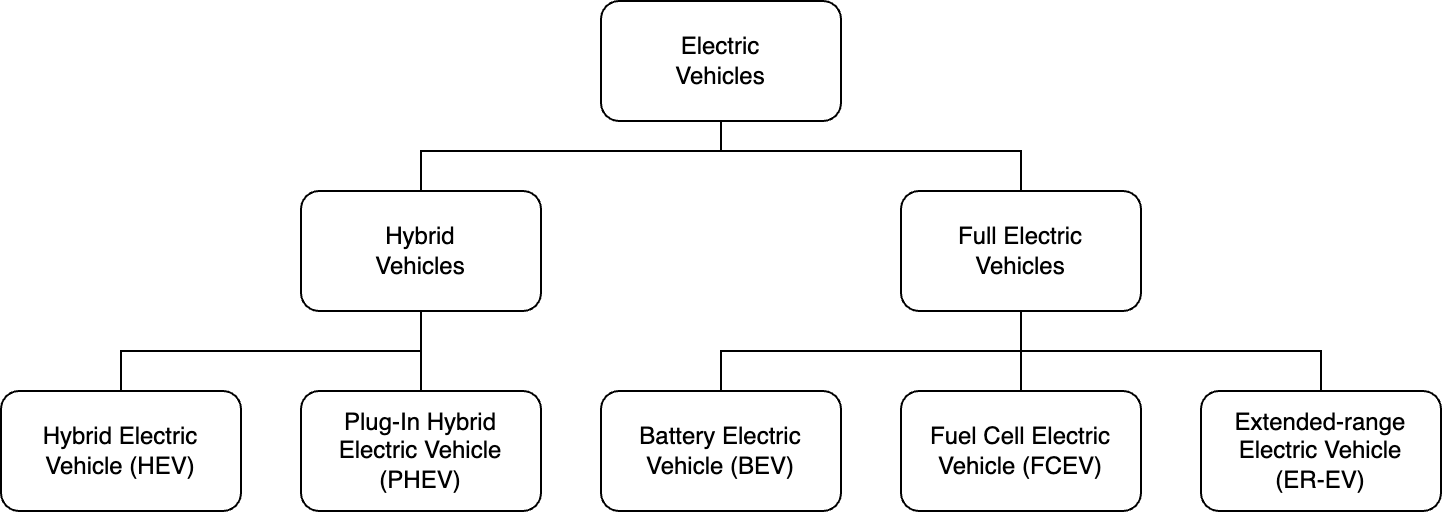
\includegraphics[width=0.8\textwidth]{resources/images/main/1_fundamentals/ElectricVehicleTypes.png}
    \caption{Classification approach for different \acrshort{ev} types based on \cite{acharige_review_2023}.}
    \label{fig:ev-classification}
\end{figure}

\subsection{Charging Infrastructure}
\label{ch:Fundamentals:sec:Electric Mobility:ssec:Charging Infrastructure}

To facilitate the growing number of \acrshortpl{ev}, a crucial aspect is the establishment of a broad charging infrastructure comprising multiple \acrshortpl{cs}. As highlighted in \cite{gnann_fast_2018}, the requirements for charging infrastructure are highly variable, depending on the battery capacity and charging rate, which is predicted to increase in the future.
In order to satisfy the various power requirements and to cover the wide range of vehicles and used batteries, a heterogeneous range of \acrshortpl{cs} exists.
From stations providing so--called slow charging with a power supply up to 22 kW, more advanced technologies allow fast charging \acrshortpl{cs} for power requirements above this certain range. \\
\noindent For a better understanding of the different scenarios in which a \acrshort{cs} could be used for charging, this work divides the infrastructure and the corresponding stations into three different groups. 
These groups, classified according to accessibility level for the \acrshortpl{evu}, are presented in Table \ref{tab:cs-accessibility-levels} alongside their user restrictions, the associated locations, and most commonly used charger levels:

\begingroup
\setlength{\tabcolsep}{10pt} % Default value: 6pt
\renewcommand{\arraystretch}{1.5} % Default value: 1
\begin{table}[h]
\centering
\caption{Differentiation of accessibility in case of charging opportunities based on \cite{kathiresh_e-mobility_2022},\cite[18-19]{linnemann_elektromobilitat_2020}.}
    \begin{tabular}{c|c|m{5.5cm}|c}
    Accessibility & Restrictions & Location & Charging Level \\ \hline
    Public & No & fleets, highway, distribution centers & 3 \\
    Semi--Public & Yes & workplace, hotels & 2 \\
    Private & Yes & private households & 1 
    \end{tabular}
\label{tab:cs-accessibility-levels}
\end{table}
\endgroup

\newpage

\noindent Alongside the separation according to the accessibility level, a differentiation based on classes of \acrfullpl{cs} is possible. For a detailed illustration of the dependencies and relationships between the different classes, see Figure~\ref{fig:charging-station-classification} below. 

\begin{figure}[h]
\centering
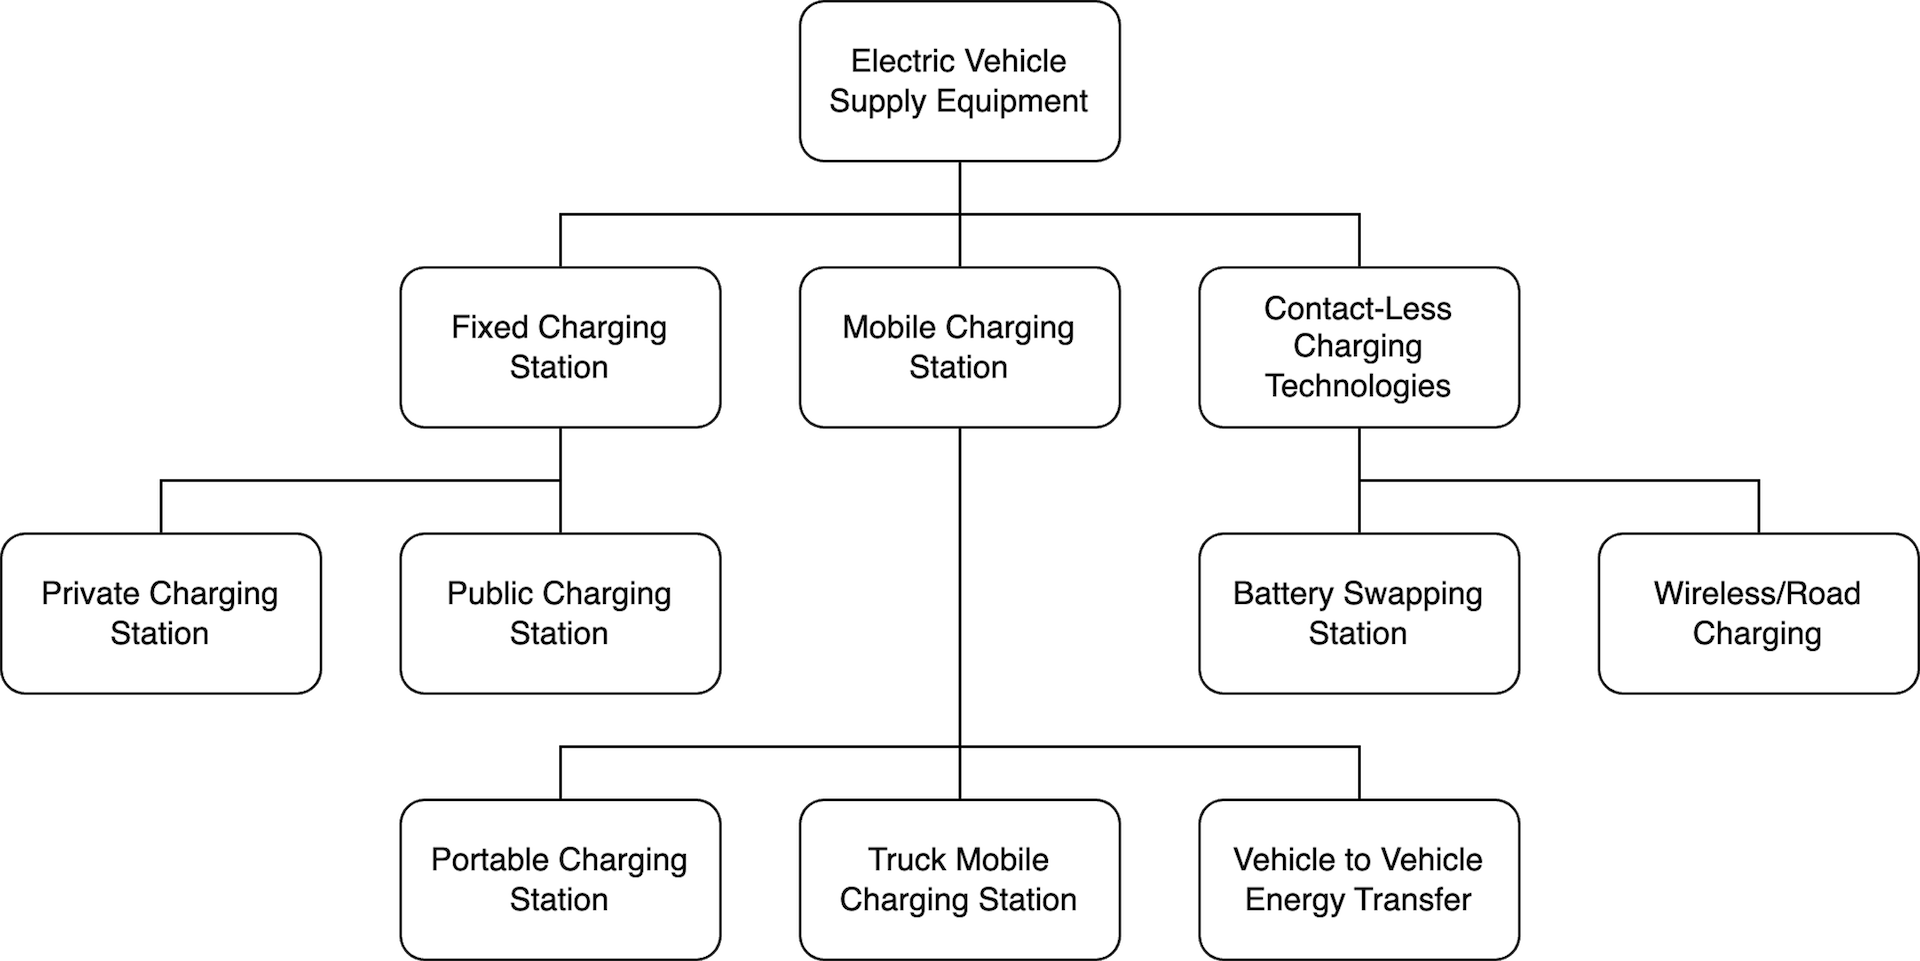
\includegraphics[width=0.8\textwidth]{resources/images/main/1_fundamentals/ChargingStationClassification.png}
\caption{Classification for different types of \acrshortpl{cs} based on \cite{afshar_literature_2020}.}
\label{fig:charging-station-classification}
\end{figure}

\noindent To provide a more detailed view on the infrastructure and the hardware used for charging, also referred to as \acrfull{evse}, all components and systems necessary to supply electric power from the grid to the battery of an \acrfull{ev} are explained afterwards.
Beginning with the \textbf{\acrfull{cs}} itself, as physical power unit the \acrshort{ev} is connected to. As mentioned above, \acrshortpl{cs} can vary in size and complexity, ranging from small wall--mounted units designed for home use to more extensive public \acrshortpl{cs} found in parking lots, shopping centers or along highways. 
To establish a connection between grid, \acrshort{cs} and car, a \textbf{Connector or Charging Cable} is needed. It contains plugs on both ends, which are connecting to the vehicle's charging port and to the \acrshortpl{cs} outlet. 
As an integral part of the \acrshort{evse}, the \textbf{\acrshort{pms}} regulates the flow of electricity from the grid to the vehicle's battery. It ensures safe and efficient charging, managing the power level based on the vehicle's battery capacity and the grid's capacity.
Allowing the communication between the \acrshort{ev}, the \acrfull{cs}, and the grid, a \textbf{\acrshort{cms}} is used as a backend. It allows data exchange regarding charging status, electricity prices, user authentication, and other relevant information.
In the case of public \acrshortpl{cs}, a payment and authentication system is usually integrated into the \acrshort{evse}. This system verifies the user's identity, authorizes the charging session, and processes payment for the electricity consumed.
On top of the described components, various safety features are integrated to protect users, the vehicle, and the surrounding environment. Including features such as ground fault protection, over--current protection, temperature monitoring, and emergency shut--off capabilities~\cite{littlefuse_designing_2020}.
\noindent To meet the wide range of existing \acrshortpl{ev} and their individual power requirements, different categories of chargers have been established based on the power level provided. This work lists the most notable categories, along with their specifications and typical usage, in Table~\ref{tab:ev-charging-levels}. 

\begingroup
\setlength{\tabcolsep}{10pt} % Default value: 6pt
\renewcommand{\arraystretch}{1.5} % Default value: 1
\begin{table}[h]
    \centering
    \caption{Listing of different \acrshort{ev} charging levels based on \cite{acharige_review_2023}.}
    \begin{tabular}{c|c|m{6.5cm}}
        Charging Level & Charging Power & Use Case \\ \hline
         1 & 1.44 kW -- 1.9 kW & Typically the slowest charging option and suitable for overnight charging at home \\
         2 & 3.1 kW -- 19.2 kW & Provides faster charging compared to Level 1 and is commonly used for home charging setups and public charging stations \\
         3 & 20 kW -- 350 kW & Fast charging operates at a higher voltage, directly charging the vehicle's battery with direct current power. Commonly used in public fast--charging stations.\\
         \acrshort{xfc} & >350 kW & Ultra--fast charging provides fastest charging option. Commonly used in commercial settings. 
    \end{tabular}
    \label{tab:ev-charging-levels}
\end{table}
\endgroup

\newpage

\subsection{Battery Technology}
\label{ch:Fundamentals:sec:Electric Mobility:ssec:Battery Technology}

For storing the required energy, \acrshortpl{ev} rely on their built--in batteries. As key components inside an \acrshort{ev}, they have to handle high energy capacity and high power, within limited weight and space to affordable prices.
Therefore, most manufacturers use Lithium--ion batteries in their cars nowadays. 
Alternatives such as \textit{Lead Acid} and \textit{Nickel--based} batteries usually have lower durability compared to lithium--based batteries due to their shorter lifespan and subsequent inadequate performance in extreme weather or higher discharge rates \cite{acharige_review_2023}.
Generally, the advances in this technology leading to an increase in the range of the \acrshortpl{ev} and a reduction in the charging time, combined with cost effectiveness, are an essential part of the transition from cars using \acrshort{ice} to purely \acrshort{ev}.

\subsection{Relevant Standards}
\label{ch:Fundamentals:sec:Electric Mobility:ssec:Relevant Standards}

To establish a comprehensive interface for information exchange between \acrshortpl{cs}, \acrshortpl{ev}, and their users, various organizations, initiatives and the industry have established several standards for communication between the single actors in this particular environment.
Aside from the \acrfull{ocpp} \cite{noauthor_ocpp_nodate}, a communication protocol, developed by the \acrfull{oca} \cite{noauthor_open_nodate}, other protocols and specifications exist, covering different aspects and scenarios relevant during or before the charging process.
In addition to the previously mentioned \acrshort{ocpp}, further standards relevant to this work are listed and explained below.

\subsubsection{Open Charge Point Protocol}
\label{ch:Fundamentals:sec:Electric Mobility:ssec:Relevant Standards:sssec:OCPP}

The \acrfull{ocpp} outlines an open industry--standard communication protocol, used especially in charging infrastructure for \acrshortpl{ev}. Proposed by the ElaadNL foundation as an open protocol to support the communication between \acrshort{cs} and the related backend services, the ownership was transferred to \acrshort{oca} in 2014 \cite{garofalaki_electric_2022}.
In general, the \acrshort{ocpp} is designed to provide interoperability and seamless integration between different \acrshort{cs} vendors and network operators, ensuring that \acrshort{ev} drivers can charge their vehicles at any compatible \acrshort{cs}.
Therefore, it is maintained by the \acrfull{oca}, a consortium of \acrshort{ev} charging infrastructure stakeholders, as an open protocol and not proprietary to any specific manufacturer or organization. 
In this way, it is ensured that the \acrshort{ocpp} remains a collaborative and evolving standard \cite{noauthor_ocpp_nodate}. \\
From an architectural point of view, the protocol could be described in the form of a client/server architecture. The \acrshort{evse} in this model acts as the client, while the \acrshort{csms} serves as the server. 
The server responds to the client's requests and manages the charging processes accordingly. This request--response model, where the client sends requests to the server, and the server responds with the appropriate information or action enables real--time communication between the \acrfull{cs} and the connected \acrfull{cms}.
As an interface for communication, two different types of protocols are used. On the one side, the WebSocket protocol, described in \ref{ch:Fundamentals:sec:Data Exchange:ssec:WebSocket}, for bidirectional communication, providing a persistent connection between the \acrshort{evse} and the \acrshort{cms} allowing a faster and more efficient data exchange. On the other side, \acrfull{soap}, as described in \ref{ch:Fundamentals:sec:Data Exchange:ssec:SOAP}, is suitable for the implementation of one--way communication between the respective entities.
To differentiate between particular feature sets, the \acrshort{ocpp} is versioned. 
The versions are presented as floating point numbers, which increase with major or minor releases within the nomenclature, such as \acrshort{ocpp} 1.6 and \acrshort{ocpp} 2.0. Representing the latest versions of the protocol, which are widely used in current implementations. \\ \\
\noindent For the communication between \acrshort{cs}, \acrshort{csms} and the \acrshort{evu}, the \acrshort{ocpp} protocol relies on so called operations. Each of these operations describes a set of instructions, which are necessary to fulfill and successfully complete the underlying process.
According to the required operations used in the context of this work, a subset of operations are selected, which are elucidated in the following list. 
The wording and the explanations are based on the standard documentation for the \acrshort{ocpp} version 1.6 \cite{noauthor_ocpp_nodate}:

\begin{description}
    \item[Authorize] Before starting a charging session, the \acrshort{evu} \acrfull{rfid} card or other identification is sent to the central system for authorization. The \acrshort{cms} checks the driver's credentials and responds with an authorization status.
    \item[Start Transaction] After successful authorization, the \acrshort{cms} sends a start transaction request to initiate the charging process. The \acrshort{cs} acknowledges the request, and the charging session begins.
    \item[Status Notification] The \acrshort{cs} may send status notifications to the \acrshort{cms} to update the current state of the \acrshort{cs}, such as \verb|Available|, \verb|Charging|, \verb|Reserved|, or \verb|Faulted|.
    \item[ReserveNow] In case a user needs an available connector on a \acrshort{cs}, he could send a \textit{ReserveNow} request via the \acrshort{cms} to the \acrshort{cs}, which reserves one specific or at least one connector on the station for a specified duration. The according connector in case of successful reservation changes from status \verb|Available| to \verb|Reserved|.
    As a result, only the user assigned to the deposited \acrshort{rfid} card is able to start charging at the specified connector or the superior \acrshort{cs}.
    \item[Cancel Reservation] For canceling the created reservation the user has the ability to manually send a request with the assigned reservation \acrshort{id} to the \acrshort{cms}, to free the connector again. Otherwise, the \acrshort{cs} will notify the \acrshort{cms}, if the reservation reaches its expiry limit.
\end{description}

\subsubsection{Open Charge Point Interface}
\label{ch:Fundamentals:sec:Electric Mobility:ssec:Relevant Standards:sssec:OCPI}

\acrfull{ocpi} is a standardized, open protocol facilitating communication and supporting interoperability between different charging network operators, which provides \acrshort{ev} drivers with access to charging infrastructure from multiple providers. This is achieved by utilizing a harmonized approach. 
Alongside \acrshort{ocpi}, other proposals regarding the development of cross--border \acrshort{ev} travel, also known as \textit{e--roaming}, exist. 
The most prominent ones are \acrfull{oicp}, \acrfull{ochp} and \acrfull{emip} \cite{ferwerda_advancing_2018}. 
In contrast to the \acrshort{ocpi}, they are all developed by proprietary institutions and integrated inside their offerings providing dedicated roaming platforms. 
Thus, no way is provided to allow compatibility, making the \acrshort{ocpi} standard more suitable in the case of openness and interoperability. \\
\noindent In case of available features, \acrshort{ocpi} provides defined endpoints, used for communication between \acrshort{cs}, \acrshortpl{cms}, \acrshortpl{emsp} and \acrshortpl{cpo}. These endpoints include functionalities such as location discovery, charge point data, authorization, charging sessions, and error handling. 
For integrating \acrshort{ocpi} into existing software systems it is heavily based on the paradigm of \acrfull{rest}. This allows communication via standard HTTP methods utilizing \acrfull{json} as a data format for transmitting information. 

\noindent The listing below provides a short overview of available features and functionalities provided by \acrshort{ocpi} \cite{noauthor_open_2021}:

\begin{description}
    \item[Location Discovery] Charging networks can exchange information about available charging locations, providing details such as location coordinates, \acrshort{cs} types, and status.
    \item[Charge Point Data] Access to data on \acrshort{cs}, including details on availability, status, and pricing, is possible through \acrshort{ocpi}.
    \item[Charging Sessions] \acrshort{ocpi} supports real--time information about ongoing charging sessions, including start time, energy consumed, and current charging status.
    \item[Authorization and Authentication] In combination with their respective \acrshort{cpo} accounts or other authentication methods \acrshortpl{evu} are able to authenticate themselves to access charging services.
    \item[Remote Start/Stop Charging Sessions] To initiate charging sessions, \acrshortpl{evu} are capable of remotely starting and stopping their current charging sessions. This allows the driver to initiate charging sessions via their mobile apps or other remote means.
    \item[Tariff Information] Charging networks can share pricing and tariff information, providing transparency to \acrshortpl{evu} about the cost of charging at different locations.
\end{description}

\subsubsection{ISO 15118}
\label{ch:Fundamentals:sec:Electric Mobility:ssec:Relevant Standards:sssec:ISO 15118}

To meet the demands of \acrshortpl{evu} and address the problems of lack of standardization in charging infrastructure interoperability and information exchange between grid \acrshort{evse}, \acrshort{ev} and \acrshort{evu}, Daimler and RWE started a collaboration in September 2009 to enable Smart Charge Communication.
Until its initial release as the standard for Plug--n--Charge connections in June 2014, further progress towards the standardization of charging infrastructure communication was carried out \cite{heinrich_iso_2017}.
Nowadays, this standard consists of multiple parts. From the analysis of the underlying use cases to a description of requirements for the communication over the different \acrshort{osi} layers, it describes \acrshort{poi}--data, the \acrshort{cs} availability, payment, communication standards as well as the \textit{Plug \& Charge} or \textit{e--Roaming} approach \cite{brosi_methode_2019}. 
However, the required level of data granularity or quality is not specified \cite{linnemann_elektromobilitat_2020}. Considering these gaps that still exist in the \acrshort{iso} 15118, it is far from being complete and requires further development and adaptation.

\subsection{Smart Charging}
\label{ch:Fundamentals:sec:Electric Mobility:ssec:Smart Charging}

The concept of smart charging or intelligent charging is a systematic approach that optimizes the charging process of \acrshortpl{ev} to be more efficient, cost-effective, and environmentally friendly using information and communication technologies. 
Therefore, the subsequent calculations consider factors such as electricity demand, grid capacity, availability of renewable energy, and individual user preferences to allow for optimizations in the user's decision--making \cite{deb_smart_2022}.
One of the primary goals of this methodology is to balance the demand on the underlying grid, affected by charging large numbers of \acrshortpl{ev} simultaneously \cite{daina_electric_2017}. Especially during peak hours increased electricity costs or potential blackouts could occur. 
In order to mitigate these situations, smart charging takes the current load of the grid into account and adjusts the possible charging rates based on the given constraints to prevent overloading the grid and optimizing the use of available energy \cite{garcia-villalobos_plug-electric_2014}. 
Compared to the unidirectional charging method originally known as \acrfull{v1g}, the approach of \acrfull{v2g} enables smart charging systems to charge bidirectionally between the \acrshortpl{ev} battery and the grid \cite[199]{kathiresh_e-mobility_2022}. Allowing \acrshortpl{ev} with sufficient battery capacity to return energy to the grid during times of high demand and turning them into mobile energy storage units to enhance grid stability and resiliency.
To offer all these functions, smart charging relies on data connectivity and communication between the single \acrshortpl{cs}, the \acrshortpl{ev}, and the underlying grid, which makes it vulnerable to malign third--party entities as well. On the other side, these factors can contribute to better grid management overall, giving grid operators insight into electricity demand patterns and enabling them to plan grid upgrades accordingly.

\subsection{Smart Grid}
\label{ch:Fundamentals:sec:Electric Mobility:ssec:Smart Grid}

More generally, the terminology of a \acrfull{sg} describes the characteristics of an intelligent system that deals with high energy consumption in order to increase energy reliability and the corresponding costs \cite{sharma_smart_2020,moreno_escobar_comprehensive_2021}.
It consists of multiple parts, like a sufficient infrastructure, applications, and several technologies to manage the energy flow inside the grid.
This includes, for example, monitoring and measuring solutions as important cornerstones, allowing the grid to support an efficient generation and distribution of power. Supplemented by the behavior of the users connected to the \acrshort{sg}, which is a component of the continuously operating optimization procedures.
Based on \cite{moreno_escobar_comprehensive_2021}, researchers have identified 94 potential optimization algorithms thus far, primarily implemented in central orchestration systems and observing the \acrshort{sg} to manage these kinds of distributed networks.
As a result, the smart grid is capable of dynamically and intelligently controlling the flow of power based on predetermined objectives to meet the needs of all nodes in the network. 
Considering the delivery of electricity, compared to existing grids that deliver power in one direction only, smart grids enable bi--directional power delivery.  
Therefore, the smart grid utilizes \acrshort{der}, such as \acrshortpl{ev} or renewable energy sources, located at consumer homes, to absorb surplus power when not in use.
This approach is very similar to the \acrshort{v2g} functionality of smart charging described in \ref{ch:Fundamentals:sec:Electric Mobility:ssec:Smart Charging} and could be combined with it.

\section{Reservation Systems}
\label{ch:Fundamentals:sec:Reservation Systems}

Originally, current reservation systems were developed as \acrfull{crs} to facilitate collaboration between airlines and technology companies \cite{xiang_evolution_2020}. The original objective of the system to be a tool to book resources without the need for paper or other management systems has obviously evolved over time.
This also applies to the features and abilities of these systems.
Started as a centrally managed system with restricted access to call center operators, which administered the available resources for their corresponding airlines or hotel chains, the further development of the world wide web in 1989 led to a transformation away from the \acrshort{crs} to online booking systems, also known as web--based \acrfullpl{ibe}, directly available to the customer via their personal computers at home.
In general, a reservation system could be defined as a software application or platform that facilitates the process of booking and securing limited services, resources, or accommodations in advance, based on the definition of Xiang et al. \cite[p.~2]{xiang_evolution_2020}. 
As mentioned previously, besides its original application in the travel or hospitality industry, it is also a common tool for the administration of the transportation or entertainment industry. With the goal of simplifying reservation procedures for customers and minimizing administrative tasks, while increasing user satisfaction.
Based on the system architecture and the technologies employed, reservation systems could vary depending on the functionalities required. When utilized in a web-based application, such as an online booking system, it is essential to consider different constraints and use cases, compared to a local system within one institution. 
To abstract from the requirements necessary for particular deployment scenarios, the following section outlines a set of fundamental characteristics and functionalities that a reservation system should typically encompass. While the chosen list of features may not include all the use cases required for a specific system, it should furnish a brief overview for general purposes.
For reference and guidance in the case of the functionality of the reservation system, the existing research and literature on hotel reservation systems such as \cite{delizo_online_2013,bemile_online_nodate} as well as the common functionalities found in current booking systems are used.
\textbf{Booking and Scheduling} could be described as the main purpose of a reservation system. By using this feature users can view available dates, times, or slots and make reservations for specific services, activities, or resources. The system ensures that conflicting bookings do not occur.
To provide an overview, which represents the availability of the aforementioned resources, the system requires \textbf{Real--Time Availability}. Therefore, users can see immediately if the desired service or resource is available for the chosen date and time.
For the purpose of personalizing the user experience, retaining reservation history, and enabling loyalty rewards, the common reservation application provides a \textbf{User Registration and Authentication} feature to allow the user to create an account or log into restricted areas of the system to book a reservation.
Additionally, managing and monitoring bookings, the option to securely pay for allocated properties using a credit card or digital wallet via \textbf{Online Payments} often is part of the service offering.
To acknowledge successful reservations or notify users of any changes to their bookings, a \textbf{Confirmation and Notifications} should be embedded in the application. This feature not only acts as a confirmation of the booking, but also evidence of the completed transaction and may contain information such as booking \acrshort{id}, date, time, and location.
Regarding the need for modification or cancellation of the reservation, the system should provide \textbf{Cancellation and Modification} features, enabling the user to cancel or modify their reservations within a specified time frame. Additionally, cancellation policies eventually exist for penalties punishing late cancellations.
Moreover, apart from the management of the reservations made through the system, it should provide a \textbf{Inventory Management} for the owners of the resources and help them manage their possessions.
Other features such as \textbf{Reporting and Analytics} or the \textbf{Integration with Other Systems}, which allow the generation of reports on booking trends, revenue, and occupancy rates, are advanced functionalities typically not visible to the end--user. Mostly offered as an administrative service extending the basic use of the system, reporting and third--party integration of other systems, such as customer relationship management (CRM), is not part of every software suite. 
This also applies to the integration of payment gateways.

\section{Data Exchange}
\label{ch:Fundamentals:sec:Data Exchange}

After the presentation of the various services, their corresponding communication channels, and the information provided within Section \ref{ch:Fundamentals:sec:Electric Mobility:ssec:Relevant Standards}, the subsequent Section deals in more detail with the technical concepts that underlie both the protocols and the application.
In addition to a brief overview of \acrfull{rest} in \ref{ch:Fundamentals:sec:Data Exchange:ssec:REST}, a quick summary of the technologies \acrfull{soap} in \ref{ch:Fundamentals:sec:Data Exchange:ssec:SOAP}, \acrfull{odata} in \ref{ch:Fundamentals:sec:Data Exchange:ssec:OData} and WebSockets in \ref{ch:Fundamentals:sec:Data Exchange:ssec:WebSocket} follows. 

\subsection{REST}
\label{ch:Fundamentals:sec:Data Exchange:ssec:REST}

Introduced by Roy Fielding as an architectural style \cite{patni_pro_2017} to design distributed systems, \acrfull{rest} provides concepts and a set of constraints that define resources accessed via a common interface by \acrshort{http} methods specified in the standard protocol description.
Stated as the general set of \acrshort{http} methods used to query a \acrshort{rest} \acrfullpl{api}, the methods \verb|GET|, \verb|POST|, \verb|PUT| and \verb|DELETE| are the most conventional examples in the context of web development. 
Representing a set of standardized operations, also known as \acrshort{crud} operations, similar to the functionalities utilized in the context of relational and non--relational databases, these methods assume the activation of certain functionalities within the respective targets.
The verbs used to name the operations carry significant meaning, indicating the associated functionality and the expected outcome of the call.
Aside from the mere retrieval of data, which is usually performed by the use of \verb|GET|, the creation and update of an entity involves either \verb|POST| or \verb|PUT|.
Intentionally, while awaiting a specific result from performing a read operation, creation methods may or may not return the resulting object. Both possibilities align with the standard and result in subtly different behaviors due to varying design decisions, such as prioritizing reducing network bandwidth versus usability.
To determine the appropriate targets for the client, \acrshort{rest} defines the concept resources, which allows a resource identifier to be mapped in the form of a \acrshort{uri} or a \acrshort{urn}. Following this pattern, a legitimate resource representing a car is presumably indicated by the  \verb|http://rest.service.com/cars|. 
Sending a \acrshort{http} request with the \verb|GET| method to this resource should result in a list of cars provided by the service. As a valid format for representing data, both \acrshort{json} and \acrshort{html} documents are permissible. Even images could be utilized.
Further data elements defined by \acrshort{rest} are resource metadata, representation metadata, and control data, which are only mentioned here for completeness. 
In addition to these core components, \acrshort{rest} provides numerous options for application and system design. However, they are not relevant to this research and are therefore not described in detail here.

\subsection{SOAP}
\label{ch:Fundamentals:sec:Data Exchange:ssec:SOAP}

As a counterpart to the \acrshort{rest} protocol described in the previous Section \ref{ch:Fundamentals:sec:Data Exchange:ssec:REST}, \acrshort{soap} was created by Dave Winer and others in collaboration with Microsoft \cite{patni_pro_2017} to addresses the demands of enterprise software.
The fundamental idea of \acrshort{soap} is to provide data as services, tagged with names consisting of both verbs and nouns. For instance, the service named \textit{getCar} is exclusively for providing information about cars and is not intended for any other objectives.
In contrast to \acrshort{rest}, this ensures better communication of the purpose for which the method is intended, as well as the necessary data that this particular function relies on to fulfill its purpose. All of this information about the handled objects and parameters is communicated to the client prior to the actual interaction and described as part of a \acrfull{wsdl} document, which is publicly available from the \acrshort{url} of the particular services implementing this protocol.
This creates a so-called contract between a server and a client, providing security and authorization as well as more direct access to objects available on the server. As a result, these components are much more tightly coupled.
Therefore, \acrshort{soap}, as outlined in \cite[4]{patni_pro_2017}, is typically recommended for scenarios involving use cases considering transactional operations or in case the environment is dependent on this protocol.

\subsection{OData}
\label{ch:Fundamentals:sec:Data Exchange:ssec:OData}

Another option for implementing web--based services besides utilizing only the \acrshort{rest} architectural style is the \acrshort{odata} protocol, which aims to build on top of the latter to provide both a higher level of consistency in terms of breaking changes and to increase interoperability between the communication partners \cite{noauthor_documentation_nodate}.
To accomplish these goals, \acrshort{odata} services, similar to services implementing \acrshort{soap}, supply a metadata definition using \acrfull{csdl} as a metadata description language ensuring a machine-readable form of the service functionalities it provides.
In the case of generic clients with no knowledge of the implemented logic of the services, these documents exchanged as part of a preflight request between server and requestor, give the clients the ability to interact in a formalized way.
Alongside these outstanding features, the \acrshort{odata} standard offers additional concepts such as \textit{namespaces} or specific \acrshort{url} conventions to cover much more advanced scenarios. 
Nevertheless, these aspects are beyond the scope of this informative Section and are not covered in this brief introduction.

\subsection{WebSocket}
\label{ch:Fundamentals:sec:Data Exchange:ssec:WebSocket}

Based on the RFC 6455 standard \cite{melnikov_websocket_2011}, the WebSocket protocol facilitates two--way communication between a client and a remote host. Formerly, clients on the web who needed to establish bidirectional communication with their server had to utilize \acrshort{http} calls to request updates from their correspondent and send notifications in response.
Resulting in numerous obstacles for the server and its client, including the quantity of open \acrfull{tcp} connections and the overhead generated by the bloating headers appended to each request.
Trying to solve these problems, the WebSocket protocol suggests using only one \acrshort{tcp} connection for traffic in both directions.
In order to create this information channel, Fette and Melnikov's proposal allows taking advantage of existing infrastructure, which lets the users replace existing technologies using \acrshort{http} as the transport layer within their applications.
To initiate the data exchange process, this communication approach relies on establishing trust through exchanging preliminary handshakes and utilizing the origin--based security model, which is commonly implemented in current browser applications.
Once the trust between server and client is established, the protocol allows the applications to communicate utilizing basic message framing layered over \acrshort{tcp} stack. This grants web-based services the ability to construct efficient information exchange in two directions, without the need to open multiple \acrshort{http} connections.
Apart from the possibility of using the WebSocket protocol over unencrypted \acrshort{http} channels, it can be utilized in encrypted traffic via \acrfull{https} on port 443 as well.

%% LaTeX2e class for student theses
%% sections/main/2_requirements_engineering.tex
%%
%% Karlsruhe University of Applied Sciences
%% Faculty of  Computer Science and Business Information Systems
%%
%% --------------------------------------------------------
%% | Derived from sdqthesis by Erik Burger burger@kit.edu |
%% --------------------------------------------------------

\chapter{Requirements Engineering}
\label{ch:Requirements Engineering}

The main focus of this chapter is to describe the requirements that a reservation system for charging infrastructure needs to fulfill.
For that purpose, this work uses a fictional scenario to paraphrase and describe the underlying problem. Furthermore, a comprehensive representation of significant edge cases the system design has to consider is depicted as well as an accentuation of highlight potential problems is included.
Adapted from the requirements, use cases and goals are defined, giving an overview of the central tasks of this thesis.

\section{Scenario}
\label{ch:Requirements Engineering:sec:Scenario}

Beginning with the capture of fundamental points necessary for outlining the scenario, which represents the problem space the system is intended to operate.
The scenario includes, besides the location where the subsequent setting takes place, a group of personas describing fictional people representing actors, who interact with the system itself.
Each of these actors has different demands due to their current life situations regarding the usage of the system, which results in different expectations with respect to the fulfillment of their goals, based on the interaction with the system.
Formalizing these expectations and transforming them in a more general way, they could be derived as use cases separated by system actors for the implementation afterward.

\noindent To cover a broad range of possible users according to age, social backgrounds, and the ease of handling obstacles generated by new technologies, the scenario takes place in the context of the institution \acrfull{hka} located in the city of Karlsruhe.
As a partner of the \textit{Green4Ever} project \cite{noauthor_hka_nodate}, the \acrshort{hka} covers several aspects, which could be used for designing a sophisticated scenario. Aside from a broad range of users, ranging from students to the regular staff, it consists of multiple campus sites distributed all over the city.
This allows members of the institution to travel between the single sites and generate persistent demand for charging possibilities during the whole day.
Relevant for the description of the single actors, this scenario includes the sites \textbf{main campus}, \textbf{campus Amalienstraße}, also known as \textit{field office Amalienstraße}, and the \textbf{\acrfull{ltc}} with the amount of applicable \acrshortpl{cs}, which are listed in Table \ref{tab:campus-sites} below.

\begingroup
\setlength{\tabcolsep}{10pt} % Default value: 6pt
\renewcommand{\arraystretch}{1.5} % Default value: 1
\begin{table}[h]
    \centering
    \caption{Campus sites and parking lots (site areas) in the \acrshort{hka} organization with the according number of available \acrshortpl{cs}.}
    \begin{tabular}{c|c|c}
        Site & Site Area & Number of \acrshortpl{cs} \\
        \hline
        Linder Technologie Campus & Private Parking Lot \acrshort{ltc} & 1 \\
        Linder Technologie Campus & Parking Lot \acrshort{ltc} & 3 \\
        Field Office Amalienstraße & Parking Lot Amalienstraße & 3 \\
        Main Campus & Parking Lot Steinbeishaus & 3 \\
    \end{tabular}
    \label{tab:campus-sites}
\end{table}
\endgroup

\newpage

\noindent Furthermore, this work assumes the preferred way of movement to the sites is by public transportation or with their own cars.
As mentioned before, each of these campuses has its own parking lots equipped with a limited amount of \acrshortpl{cs} for students and the staff working at this site. Corresponding to the accessibility level declared in \ref{tab:cs-accessibility-levels}, the parking possibilities include public and semi--public charging opportunities.
Public parking lots and the corresponding \acrshortpl{cs} are available for students and staff members as well. In the case of semi--public parking lots, the access is only limited to visitors or staff exclusively. \\
Concerning the possibilities to configure \acrshortpl{cs}, all public stations are enabled for reservations. To prevent unnecessary complexity, this scenario does not include \acrshortpl{cs} without support for the reservation feature.
For administration and management of these facilities and the restricted charging resources, a software solution called \textit{Open e--Mobility} \cite{noauthor_github_nodate,noauthor_github_nodate-1,noauthor_github_nodate-3} is used, which includes a mobile application for the \acrshortpl{evu} and a web--based application for browser access, mostly used by administrative departments of the \acrshort{hka}. 
On behalf of these applications, the users have the possibility, according to their roles in the system listed in Table \ref{tab:system-role-collection}, to start or stop current charging sessions remotely or check for occupied \acrshortpl{cs} on the available sites and site areas.
Using privileged access via an administrative account, the user is able to deactivate or block connectors of specific \acrshortpl{cs}, to make them inaccessible until reactivation or a rebooting process.
By now, the administrator or the common user does not have the opportunity to reserve an available \acrshort{cs} connector in advance. Rather for themselves or on behalf of a specific user. This includes reservations for visitors arriving later or during times with high loads as well.
As an implication of this missing feature, a \acrfull{fcfs} mentality among the \acrshortpl{evu} was established, which led to decreased usage of \acrshortpl{ev} as a transportation means and an increasingly competitive behavior among the drivers.

\newpage

\section{Stakeholders}
\label{ch:Requirements Engineering:sec:Stakeholders}

According to the scenario elaborated in Section \ref{ch:Requirements Engineering:sec:Scenario} above, the following groups of stakeholders could be identified. 
Considering the subsequently defined staff, it is possible to further differentiate into two subclusters for additional clarification.
The description below provides an overview of the daily challenges members of these classes of people have to face in terms of the established implications defined by the scenario and their main objectives. \\

\noindent \textbf{Students} Representing the largest category of actors within the scenario and describing people studying at the \acrshort{hka}. Primarily, students spent most of their time on the \textbf{main campus} site, because the main part of lectures offered by the different faculties and the attendant exercises are located there.
In certain cases, some lecturers offer subjects at other campus positions, where doctoral research projects or research in general is outsourced. This involves several students each semester, commuting between the sites and generating additional demand on the existing charging infrastructure.
Due to the fact, that the number of students with \acrshortpl{ev} outnumbers the capacity of \acrshortpl{cs} at the different sites of the \acrshort{hka}, a student is typically concerned about the occupation rate of the public available \acrshortpl{cs}.
In consideration of planning their charging sessions, the students want an overview of available \acrshortpl{cs} at their campus site and want to reserve a public \acrshort{cs}, if they are available for reservation.
Therefore, they mostly rely on the mobile application offered by the institution, which serves as the main entry point for them to interact with the \acrshort{csms}. \\

\noindent \textbf{Staff} As the primary workforce of the \acrshort{hka}, the staff describes a group of people working at the institution, including roles like lecturers, cleaners, or librarians for example.
Based on their office location, they are typically assigned to one specific or several campus sites. Implicating the dedicated usage of the \acrshortpl{cs} for charging their \acrshort{ev}, available at their current working place.
In contrast to students, they have permission to access the \acrshortpl{cs} on the semi--public parking lots as well as the ones located in the public parking spaces. 
Due to the new home office regulations, staff members have the choice to work from home several days a week, which may relax the situation in regard to the high demand for charging infrastructure.
However, on office days staff members prefer to know the occupation rate of the \acrshortpl{cs} in the public or semi--public spaces and reserve a spot for a guaranteed charging possibility for their \acrshort{ev}.
Referring to the fact, that they spent most part of their daily working hours on the computer rather than their mobile, staff members utilize the web application as a primary way of managing their charging sessions.
The mobile application, the majority of the users rely on, is only used in certain cases.

\newpage

\begin{description}
    \item[Maintenance Personal] As a dedicated subset of the regular staff working at the \acrshort{hka}, the maintenance personnel consists of caretakers in the first place. Their regular occupation consists of responsibility for the maintenance of the physical infrastructure as well as service offerings respecting the charging stations located on the different campuses.
    For work--related trips between the single sites, the maintenance team makes use of a \acrshort{fev} with a dedicated \acrshort{cs} exclusively accessible by this vehicle and the respective staff.
    To monitor the connected charging infrastructure and identify outtakes due to technical errors, the caretakers interact with the system using the administration dashboard, via a personal workstation in their office. In cases where a computer is not accessible, they utilize the mobile application to check the status of the charge points.
    Besides the functionality as a supervisory system for the infrastructure, the caretakers need access to the reservations made on the \acrshortpl{cs} to resolve conflicts related to system outtakes or to manage the corresponding users.
    \item[Administration] Representing the administrative counterpart to the maintenance personnel, the group of secretaries working at the administration office manages internal data relating to staff and students belonging to the \acrshort{hka}, internal workflows, or communication with other organizations. 
    This includes paperwork in relation to certain approvals for new students, maintaining the stored records, and processing incoming requests. Among other things, they are responsible for organizing events on and around the campus sites, planning upcoming visitations from external facilities, and coordinating the utilization and maintenance tasks for the charging infrastructure.
    As a supervisory unit for the \textbf{Maintenance Personal}, they are scheduling maintenance and delegating tasks to the caretakers in case of extraordinary servicing.  
    Therefore, staff members attending these positions need access to the \acrshort{csms} similar to the scope of the maintenance staff. In contrast to the caretakers, they are not leaving their office for interaction with the \acrshortpl{cs}, therefore they do not rely on the functionalities the mobile application has to offer.
\end{description}

\section{Personas}
\label{ch:Requirements Engineering:sec:Personas}

Appropriate to the defined stakeholders in the previous Section \ref{ch:Requirements Engineering:sec:Stakeholders}, each stakeholder requires a representation as a persona in regards to a dedicated user account in front of the system.
This allows a mapping between the accounts and the existing system roles, which enables easier separation between the use cases extracted later on and the assignment to the different stakeholders. 
Hereinafter, personas prescribing individuals inside the scenario including their dedicated demands in respect of the challenges their particular stakeholder group has to face. 

\newpage

\begin{description}
    \item[Lisa Knaus] is a \textbf{Student} at the \acrshort{hka} and is studying computer science in the third semester. In respect of her current living situation, located in a village with limited access to public transportation, she primarily relies on driving by car as her main transportation means. 
    Fostered through financial benefits promoted by the different car manufacturers for young drivers with interest in acquiring an \acrshort{ev}, she sold her old car with \acrshort{ice} and switched to a \acrfull{fev}. 
    Under normal circumstances the health of the internal battery allows her to drive with a full charge from her hometown to the main campus site and back without a need to recharge. Occasionally she forgot to recharge at home and needed a charging possibility for her vehicle during the lecture time. Depending on the day and the utilization of the charging infrastructure, this is certainly a challenging task and she needs to arrive very early to get a free charging spot. 
    \item[Holger Starke] is an employee working as a member of the \textbf{Staff} at \acrshort{hka}. 
    Within the in--house server administration team, his daily tasks cover the maintenance of the server landscape, applying new versions of internal applications, and the creation of backups, securing the records of the internal user databases. 
    Thanks to the subsidies for electric vehicles from the state and his employer, he has bought a \acrshort{fev} and is using it as his main means of transport. 
    As compensation for the still missing charging possibilities at his apartment near the institution, he drives a short distance with his car every day, to use the existing charging infrastructure at the \acrshort{hka}, to recharge the batteries during working hours. 
    Therefore, he has to use the available \acrshortpl{cs} at the different campus locations without any guarantee to recharge. 
    With the increasing amount of students and coworkers arriving with \acrshortpl{ev} over time, the search for a free \acrshort{cs} becomes more and more demanding. 
    Especially scheduled service work later in the day, located at other campuses, emerge to a running the gauntlet for parking lots with \acrshortpl{cs} equipped. 
    \item[Dieter Krause] is engaged in the role of a caretaker as part of the \textbf{Maintenance Personal} at \acrshort{hka}. During his previous position, he acted as a carrier for the daily book orders for the students at the university library on the main campus site. 
    For the reduction of \acrshort{co2} the \acrshort{hka} bought a \acrshort{fev} for bridging the short distances between the various libraries within the city. 
    This confronted him with the according up- and downside of driving an \acrshort{ev} in a very early stage. 
    Missing charging opportunities and insufficient battery life were only two obstacles he had to bother with, every day. 
    This led him to the conclusion to switch positions and he took over the responsibility for the charging infrastructure maintenance and management on the campus sites to improve the situation for all involved parties. 
    Alongside the continuously increasing number of \acrshortpl{cs}, he has fostered the establishment of dedicated charging possibilities for the members of the \textbf{Staff} and introduced an exclusive \acrshort{cs} for the \acrshortpl{ev} of the \textbf{Maintenance Personal}. 
    Even on days with a high emergence of student vehicles on the public parking lots, he and his colleagues could recharge the batteries of their \acrshortpl{fev}. 
    \newpage
    \item[Nadine Funke] acts as a secretary in the \textbf{Administration} office at \acrshort{hka}. Formerly she worked at the public administration office in Karlsruhe, in the area of public parking spaces, where she had her first experience with the problems concerning the management of the charging infrastructure on public parking lots. 
    For this reason, she does not drive an \acrshort{ev} herself and uses public transportation instead. In contrast to her previous position at the public administration office, the tasks regarding the management of the \acrshortpl{cs} are, thanks to the introduced system, much more convenient and do not require a lot of manual work. 
    By accessing the \acrshort{csms} dashboard, she could filter for the wanted \acrshort{cs} and have all the information in one place. 
    However, blocking \acrshortpl{cs} for upcoming visitors is, despite the new system, still a huge overhead for the secretaries at the \acrshort{hka}. 
    Up to now, she has had to select the specific \acrshort{cs} and the corresponding connector to block it, and she has to unblock it again when the guest has arrived.
\end{description}

\section{Role Mapping}
\label{ch:Requirements Engineering:sec:Role Mapping}

To distinguish between the single users and their privileges in compliance with the range of associated functionalities, the system introduces a set of roles. Besides the role of the basic user, two variations of administrators and a user for demo purposes are provided.
For a better understanding of these privileges and their purpose inside the system, the following Table \ref{tab:system-role-collection} lists the relevant roles, their system shortages, and a brief explanation.

\begingroup
\setlength{\tabcolsep}{10pt} % Default value: 6pt
\renewcommand{\arraystretch}{1.5} % Default value: 1
\begin{table}[h]
    \centering
    \caption{Role collection provided by the system.}
    \begin{tabular}{c|c|c|m{6cm}}
        Role & System & Shortage & Description \\
        \hline
        Basic & \verb|BASIC| & \verb|B| & Standard user without administrative privileges \\
        Admin & \verb|ADMIN| & \verb|A| & User with administrative privileges inside one organization \\
        Site Admin & \verb|BASIC| & \verb|B| & User with administrative privileges for assigned sites \\
        Site Owner & \verb|BASIC| & \verb|B| & User with administrative privileges for owned sites \\
        Super Admin & \verb|SUPER_ADMIN| & \verb|S| & User with extended administrative privileges for the management of organizations and tenants \\
        Demo & \verb|DEMO| & \verb|D| & Demo user with predefined login data, primarily used for demonstration purposes
    \end{tabular}
    \label{tab:system-role-collection}
\end{table}
\endgroup

\noindent Based on the available user privileges introduced above, which are provided by the system per default, the created personas, established in Section \ref{ch:Requirements Engineering:sec:Personas}, are assigned to their corresponding roles afterward. The criteria for the assignment are primarily based on the tasks the users have to fulfill and with respect to their position inside the scenario and is presented below:

\begin{figure}[h]
    \centering
    \begin{tikzpicture}
      [
        group/.style={ellipse, draw,inner sep=-2pt,minimum height=50pt,minimum width=30pt},
      ]
      \node (b) at (0,4) {Basic};
      \node (d) at (0,3) {Demo};
      \node (a) at (0,2) {Admin};
      \node[align=center] (s) at (0,1) {Super Admin};
      
      \node (student) at (4,4) {Student};
      \node (staff) at (4,3) {Staff};
      \node[align=center] (mp) at (4,2) {Maintenance\\Personal};
      \node (admin) at (4,1) {Admin};
      
      \foreach \i/\j in {a/mp,a/admin,b/student,b/staff}
        \draw [->, shorten >=2pt] (\i) -- (\j);
      \node[fit=(a) (b) (s) (d), group,label={[label distance=5mm]above left:{\textbf{Roles}}}] {};
      \node [fit=(student) (staff) (mp) (admin), group,label={[label distance=5mm]above right:{\textbf{Groups}}}] {};
    \end{tikzpicture}
    \caption{Mapping of the roles to the group identified in the scenario described in \ref{ch:Requirements Engineering:sec:Scenario}.}
    \label{fig:role-mapping}
\end{figure}

\section{Goals}
\label{ch:Requirements Engineering:sec:Goals}

Based on the scenario and the corresponding stakeholders, the relevant goals for the resulting implementation are prescribed. As part of this work, a goal is handled as a requirement, the final product has to fulfill. 
Taking into account the different wishes in terms of the situations in which the respective stakeholders interact with the system, the following objectives could be defined. \\

\noindent \textbf{Goal 1 - Management Capabilities} As a major concern of this work the designed system, should serve as a central point for management purposes of the registered \acrshortpl{cs}. This should provide a basic set of functionalities covering specific administration tasks tailored for a certain group of users. 
Besides role mapping according to a subset of functions, the system should detect unintended usage and prohibit breach of privileges.
Furthermore, the involved users will be provided with all relevant information by the system and know their current position within the different phases of the processes at each time. \\

\noindent \textbf{Goal 2 - Self--Healing and Autonomous Processes} In case of invalid user input or violation of predefined constraints inside the processes, the system should provide mechanisms for self--healing and autonomous error handling. 
In addition to increased consistency of data within the underlying database, the ease of use of the system should be a positive side effect. \\

\newpage

\noindent \textbf{Goal 3 - Support of relevant standards} Considering the implementation of relevant communication protocols and the interoperability between different systems of \acrshortpl{cs}, \acrshortpl{ev} and \acrshortpl{csms}, the system should support well--established standards for communication and data exchange in the context of \acrshort{emobility}. 
Alongside the standards like \acrshort{ocpp} or \acrshort{ocpi}, described in the subsection \ref{ch:Fundamentals:sec:Electric Mobility:ssec:Relevant Standards}, other alternatives exist in the further evolving industry with different targets in mind. 
Considering the already implemented standard inside the underlying product, the \nameref{ch:Fundamentals:sec:Electric Mobility:ssec:Relevant Standards:sssec:OCPP} should be the protocol for the communication between \acrshort{cs} and \acrshort{csms}. \\

\noindent \textbf{Goal 4 - Modular Design} In addition to the previously mentioned goals that focus on the implemented functionality, the architectural design of the software itself should also be considered. 
As part of a system that follows both a monolithic and a microservice--based approach, multiple services interact simultaneously alongside each other. The implementation and software architecture of this work aim to avoid compromising existing functionality through poor design choices or neglected separation of concerns. 
Preferably, the new functionality should be encapsulated as part of a module, which separates the system based on its responsibilities according to the definition in \cite{clements_documenting_2011}. This should ensure easier extensibility of existing features and allow convenient maintainability.

\newpage

\section{Use Cases}
\label{ch:Requirements Engineering:sec:Use Cases}

The use cases illustrated in the use case diagram in \ref{fig:use-cases} were elaborated based on the goal definitions in the previous Section \ref{ch:Requirements Engineering:sec:Goals} and the stakeholder requirements from Section \ref{ch:Requirements Engineering:sec:Stakeholders}.
Typically, software development processes such as \acrshort{rup} \cite{kruchten_rational_1999} differ between the groups of stakeholders who have an interest in the resulting product and the actors who are actually interacting with the real system. 
As part of this scenario, the stakeholders actually represent the actors used for defining the use case in regard to interacting with the system.
The main use case, as highlighted by \textbf{goal 1}, involves managing and administering reservations within the reservation system. This encompasses creating, modifying, viewing, and deleting existing reservations made either by the users themselves or on their behalf by the administrator.
Corresponding to \textbf{goal 2}, the \textit{Scheduler} entity facilitates the required self--healing procedures. This necessitates the system to communicate with itself and employ background processes to manage forthcoming, current, and expiring reservations.
Apart from the primary focus on non--functional requirements related to \textbf{goals 3} and \textbf{4}, an additional functional requirement with reference to the selective activation and deactivation of the reservation module could be identified.
The privileges for maintenance and configuration of the particular organizations, represented as tenants inside the system, are part of the \verb|SUPER_ADMIN| role.
Usually, an external service provider outside the customer organizations is responsible for determining the scope of operation, for the service offerings provided to its customers. This role is referred to as \verb|SUPER_ADMIN|. As there is no direct interaction with the system in terms of the reservation process, there is no dedicated actor assigned to this role within the above scenario.
For comprehensively addressing all the aspects mentioned in the set goals, it is necessary to include this role with its corresponding functionality when defining the required features.

\begin{figure}[h]
    \centering
    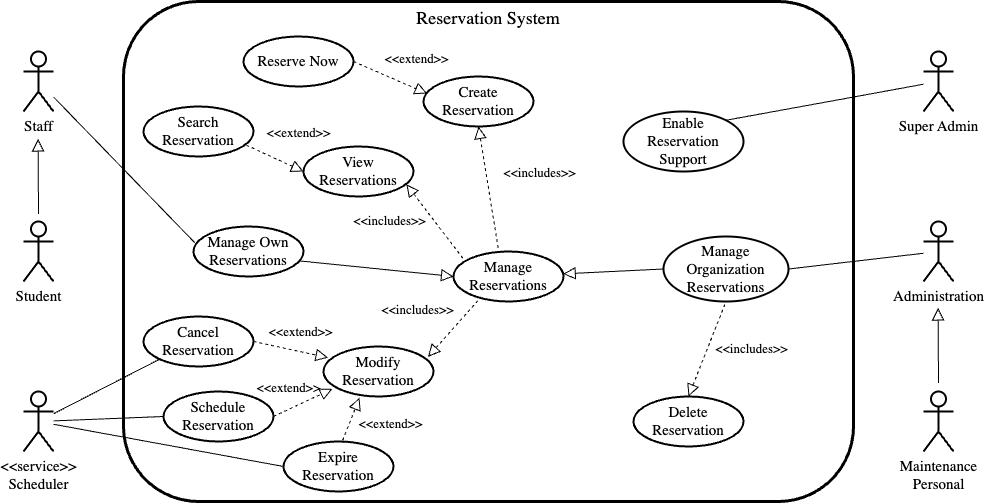
\includegraphics[width=0.8\textwidth,keepaspectratio]{resources/images/main/2_requirements_engineering/UseCases.png}
    \caption{Use Cases considering the stakeholders of the reservation system.}
    \label{fig:use-cases}
\end{figure}

%% LaTeX2e class for student theses
%% sections/main/3_approach.tex
%%
%% Karlsruhe University of Applied Sciences
%% Faculty of  Computer Science and Business Information Systems
%%
%% --------------------------------------------------------
%% | Derived from sdqthesis by Erik Burger burger@kit.edu |
%% --------------------------------------------------------


\chapter{Approach}
\label{ch:Approach}

This chapter describes the order and duration for processing the identified tasks, in accordance with the design considerations outlined in the previous chapter \ref{ch:Requirements Engineering}. 
For this purpose, this work is divided into two parts, which will later serve to classify the aforementioned challenges.
The first part is theoretical, including the paper's preparation and research to understand the problem. 
The second part afterward is practical, encompassing the tasks needed to implement the system. \\
\noindent In order to aid planning, timestamps are estimated for each task or logical unit of tasks to provide reference points during the processing of corresponding dedicated work packages. 
A logical unit, as used here, refers to a coherent cluster of individual tasks that share content or functionality and can be worked on simultaneously. Working on one task without the others would be less significant.
The standard duration for processing a task or unit is set at two weeks (10 days) typically, to ensure sufficient time for completion. The duration may differ in certain cases and is determined based on the relevance and volume of related challenges. 
After describing the two conceptual parts alongside their respective tasks and processing times, this chapter concludes with a comparison of the planned procedure with the actual one.

\section{Theoretical Part}
\label{ch:Approach:sec:Theoretical Part}

With regard to the delimitation of the problem space and the synthesis of the central problem, the main aspect of the theoretical part of this work consists of a comprehensive literature review.
This involves analyzing existing work on reservation processes used for managing \acrshortpl{cs} and allocating charging infrastructure to a specific \acrshort{evu} within a limited time frame, using various methods.
With regards to the default processing time mentioned earlier, the duration for compilation as well as analysing articles and field projects related to this area is set to one month. 
The expected result should be used as the groundwork for the subsequent practical part, which is summarised in chapter \ref{ch:Literature Review}.
As well as examining the current state of reservation systems, this review process defines a boundary for the necessary fundamentals of contextualization, resulting in the chapter \ref{ch:Fundamentals}.
Therefore, a systematic requirements engineering, taking into account the facts gathered during the research phase and the collection of baselines, using a customised scenario to select relevant use cases, results in the chapter \ref{ch:Requirements Engineering}.
Chapter \ref{ch:Design} presents the design phase, which follows the summarized requirements in chapter \ref{ch:Requirements Engineering} and the results of the literature review in chapter \ref{ch:Literature Review}. During this phase, mockups of the relevant interfaces as well as the underlying processes will be created.
With the help of these designed concepts, the actual implementation of the reservation module resulting in chapter \ref{ch:Implementation} takes place.
Subsequently, the theoretical Section concludes by validating the achieved functionality and presenting the final results, culminating in \ref{ch:Analysis and Validation}. Potential avenues for further research are also highlighted.

\section{Practical Part}
\label{ch:Approach:sec:Practical Part}

The practical part utilizes the results of the theoretical phase, as described in Section \ref{ch:Approach:sec:Theoretical Part}. Starting with the analysis of the current state of the applications used for the development of the prototypical reservation approach of this work, the final step is the implementation of the solution, taking into account the elaborated constraints and requirements.
Seven iterations covering the implementation steps for the use cases described in Section \ref{ch:Requirements Engineering:sec:Use Cases} were conducted, commencing from the end of the theoretical phase that includes four weeks of literature research and information gathering, until the end of the processing stage.
This allows for a six-week buffer to address any unforeseen features, correct any issues with the implemented logic, and complete the documentation tasks related to the theoretical part.
Following this, a list summarising the scheduled iterations and associated timeframes will be provided.

\begin{multicols}{2}
\begin{description}
    \item[Iteration 1] 18.04.2023 - 01.05.2023
    \item[Iteration 2] 02.05.2023 - 15.05.2023
    \item[Iteration 3] 16.05.2023 - 29.05.2023
    \item[Iteration 4] 30.05.2023 - 12.06.2023
\end{description}
\begin{description}
    \item[Iteration 5] 13.06.2023 - 26.06.2023
    \item[Iteration 6] 27.06.2023 - 10.07.2023
    \item[Iteration 7] 11.07.2023 - 24.07.2023
\end{description}
\end{multicols}

\noindent According to this iterative model, a functional increment of the resulting software should be provided after each iteration.

\section{Actual Course Of Action}
\label{ch:Approach:sec:Actual Course Of Action}

As there is a limited amount of available research and existing projects on reservation features for the management of \acrshortpl{cs} and charging infrastructure, the analysis and setup of the \textit{Open e-Mobility} \cite{noauthor_github_nodate,noauthor_github_nodate-1,noauthor_github_nodate-2,noauthor_github_nodate-3} solution and its particular components commenced a day earlier than planned.
Consequently, some adjustments have been made to the above timescales for the general processing of the relevant parts.
Beginning with the identification of missing functionality required for the subsequent implementation of the customized processes.
The first step was to investigate the 'e-mobility charging stations simulator' \cite{noauthor_github_nodate-3} for local simulation of a customizable charging infrastructure.
Because of the identified feature gap regarding missing reservation capabilities conforming with \acrshort{ocpp} 1.6 \cite{noauthor_ocpp_nodate}, the implementation of this crucial feature for testing and evaluation purposes was included as preliminary work for the \textit{Open e-Mobility} team.
After the team members had successfully reviewed the implemented logic and minor reworks of the code base, the changes were merged into the standard product.
Now, the extended \acrshort{cs} simulator was then used as a reservable charging infrastructure for the subsequent iterations.
Particularly, to validate the implementation of reservations compliant with version 1.6 of the \acrshort{ocpp} protocol, considering both pre-existing functionalities in the backend application and the adaptations according to this work.
This included not only the backend development but also the implementations within the frontend application during iterations three and four.
Due to the partially existing features mentioned above, the third iteration takes less time than expected, resulting in an earlier commencement of the relevant functions in the web frontend.
In light of the time savings achieved in the preceding iterations, the fifth iteration for implementing the custom reservation function began prematurely as well. 
To account for the unexpected scope of required operations alongside an end-to-end development approach, the author decided to merge the fifth and sixth iterations, resulting in an extended fifth iteration and a total of six iterations instead of the originally planned seven iterations.
Because of the previous schedule adjustments, the final iteration also started earlier and was completed later than intended. 
Primarily referring to the incidence of bugs and further requirements to manage reservations internally.
The resulting schedule, including the iterations, their specific duration, and the corresponding tasks, can be found in Table \ref{tab:development-iterations} below.

\begingroup
\setlength{\tabcolsep}{10pt} % Default value: 6pt
\renewcommand{\arraystretch}{1.5} % Default value: 1
\begin{table}[h]
    \centering
    \caption{Schedule for implementing the reservation feature designed in this study.}
    \begin{tabular}{c|c|c|m{7cm}}
        Iteration & From & To & Objective \\
        \hline
        1 & 17.04.2023 & 28.04.2023 & Feature gap detection within the existing application \\
        2 & 01.05.2023 & 12.05.2023 & Adjustments to the 'e-mobility charging stations simulator' \cite{noauthor_github_nodate-3} to support reservations complying to \acrshort{ocpp} version 1.6 \\
        3 & 15.05.2023 & 19.05.2023 & Implementation of \acrshort{ocpp} 1.6 reservation functionality in the backend application \\
        4 & 22.05.2023 & 02.06.2023 & Implementation of \acrshort{ocpp} 1.6 reservation functionality in the web frontend application \\
        5 & 05.06.2023 & 30.06.2023 & Implementation of customized reservation process in the frontend and backend applications \\
        6 & 03.07.2023 & 28.07.2023 & Implementation of \acrshort{ocpp} 1.6 reservation functionality and the customized reservation process inside the mobile application \\
    \end{tabular}
    \label{tab:development-iterations}
\end{table}
\endgroup

As well as implementing the reservation system features, this work covered other tasks related to the \textit{Green4EVer} \cite{noauthor_hka_nodate} project, although they were only indirectly connected to this work.
The decision to include these tasks is primarily based on the simplification of future deployment scenarios, such as demonstration or test cases, which require an automated and reliable setup.
Therefore, this Section mentions these tasks in addition to a brief explanation of the challenge. A detailed description is omitted from both the subsequent \textit{Design} chapter \ref{ch:Design} and the \textit{Implementation} chapter \ref{ch:Implementation} according to no direct relation to the primary problem that this work covers.

\begin{description}
    \item[Task 1 - MongoDB Manifests] As the public repository offers no other deployment options, the only available one was containerization and operation using the Docker Compose orchestration tool \cite{noauthor_overview_2023}. 
    To offer a more scalable and robust solution, the industry standard for deploying containerized applications therefore recommends employing \acrshort{k8s} \cite{noauthor_produktionsreife_nodate} as a sophisticated orchestrator. This led to this first task. 
    Nevertheless, the manifest files essential for creating a 'StatefulSets' \cite{noauthor_statefulsets_nodate} deployment, a standard way for deploying database applications inside \acrshort{k8s}, were still not yet included in the current project. 
    Hence, the MongoDB \cite{noauthor_mongodb_nodate} database's custom setup, including test data and users, already existing as part of the local setup, was employed as a blueprint for creating the necessary manifests required for the \acrshort{k8s} deployment.
    \item[Task 2 - MongoDB Helm Chart] To further reduce the effort required to deploy the database application to \acrshort{k8s} instances, the Helm \cite{noauthor_helm_nodate} toolbox and its charts for encapsulating \acrshort{k8s} manifests are integrated.  
    From the manifest files created in \textbf{task 1}, the corresponding Helm charts for the deployment are created, providing parameterization of a namespace and all required \acrshort{k8s} resources, such as 'PersistentVolumes' \cite{noauthor_persistent_nodate}, 'ConfigMaps' \cite{noauthor_configmaps_nodate} or 'Namespaces' \cite{noauthor_namespaces_nodate}. 
    \item[Task 3 - \acrshort{k8s} Deployment] For the integration of the remaining applications of the solution, additional Helm charts could be organized for the backend and the frontend application. 
    Regarding the limited resources provided by the used orchestration service, the new charts required further modifications to integrate with the MongoDB chart and the deployment restrictions of the project. This involves a shift from the predefined microservice-based deployment strategy to a monolithic approach resulting in reduced resource allocation.
    \item[Task 4 - Ingress Deployment \& Public Availability] In order to access the applications within the \acrshort{k8s} cluster, it is necessary to use an 'Ingress' \cite{noauthor_ingress_nodate} acting as a reverse proxy. 
    Therefore, this ingress must be located within the 'Namespace' the application lives in.
    Alongside the charts for the backend and frontend mentioned in \textbf{task 3}, the collection includes a configuration for deploying an NGINX ingress controller \cite{noauthor_nginx_nodate} using the \acrshort{k8s} ingress class. 
    In combination with a public \acrshort{dn} and the corresponding \acrshort{ip} address, the final stage of the \acrshort{k8s} deployment consisted of configuring the ingress deployment and registering it at a \acrshort{dn} service.
\end{description}

\newpage

\noindent As a result, the \acrshort{k8s} setup shown in \ref{fig:k8s-setup}, considers a deployment scenario that includes a custom namespace, referred to in this project as \verb|ev|, containing the particular applications, an NGINX ingress controller with a publicly accessible \acrshort{dn}, and the MongoDB database with built-in reinitialization of custom test data and users.
In terms of application distribution, only one node is used with multiple pods within the \acrshort{k8s} cluster.

\begin{figure}[h]
    \centering
    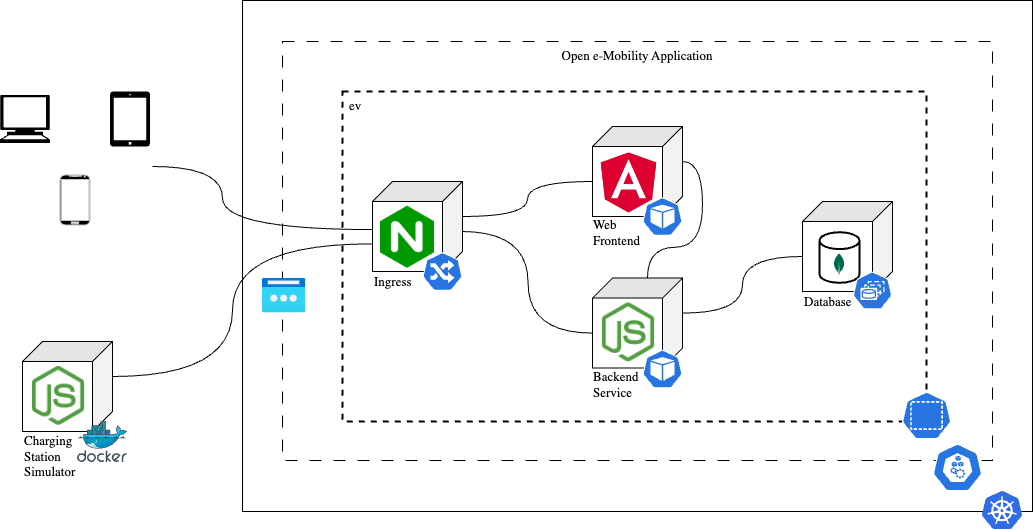
\includegraphics[scale=0.4]{resources/images/main/3_approach/KubernetesDeployment.png}
    \caption{Elaborated \acrshort{k8s} deployment architecture for the concerned solution.}
    \label{fig:k8s-setup}
\end{figure}

%% LaTeX2e class for student theses
%% sections/main/4_literature_review.tex
%%
%% Karlsruhe University of Applied Sciences
%% Faculty of  Computer Science and Business Information Systems
%%
%% --------------------------------------------------------
%% | Derived from sdqthesis by Erik Burger burger@kit.edu |
%% --------------------------------------------------------


\chapter{Literature Review}
\label{ch:Literature Review}

As the primary part of the theoretical phase described in Section \ref{ch:Approach:sec:Theoretical Part}, this chapter provides an overview of research related to the problem statement of this particular work.
Based on the existing studies, the current state of reservation systems for charging infrastructure management is identified and outlined in the last Section \ref{ch:Literature Review:sec:Current State} of this chapter.
Given the current state of implemented systems of this kind and the results of the available research, the design part in Chapter \ref{ch:Design} will use these results for the design of the system and corresponding processes implemented in this thesis.

\section{Related Work}
\label{ch:Literature Review:sec:Related Work}

In the context of supporting the wider acceptance of \acrshortpl{ev} in society, its decarbonization, and the reduction of air pollution caused by vehicles using \acrshortpl{ice} \cite{basmadjian_reference_2020}, the integration of \acrshortpl{ev} in the daily lives of citizens is still ongoing and far from being complete.
Obstacles like insufficient charging infrastructure, in comparison to the availability of gas stations, long charging times, and high investments for the public and private sectors \cite{basmadjian_reference_2020,orcioni_ev_2020} are only a few examples mitigating the end users interest in switching to \acrshortpl{fev}.
For this reason, the surrounding \acrshort{emobility} ecosystem, including the software for the interaction and management of the user, with the charging infrastructure and the convenience of the underlying processes used for the implementation, is an essential part.
Given the system landscape and protocols employed in these scenarios, the ability to reserve a \acrshort{cs} beforehand is usually lacking and has not yet been integrated into the current implementations of \acrshortpl{csms}.
As part of the comprehensive literature review in this thesis, the following selected studies describe methods for applying reservation approaches and their respective processes to current implementations. This is intended to provide an extension to the existing system landscapes and protocols in this field, with the aim of achieving certain objectives. \\
%% --------------------------------------------------------------------------------------------------------------------------------
%% An Interoperable Reservation System for Public Electric Vehicle Charging Stations: A Case Study in Germany
%% --------------------------------------------------------------------------------------------------------------------------------
\noindent In \cite{basmadjian_interoperable_2019}, the authors argued that the booking of charging infrastructure, especially for \acrshortpl{cs}, represents a pivotal role in a seamless integration of the \acrshort{cs} into the transportation and mobility sector.
Apart from the basic requirements for the design and implementation of an interoperable system, they provide a breakdown of the different advance booking approaches into four dedicated types. 
For designing their system, Basmadjian et al. used the \acrshort{emsa} \cite{kirpes_e-mobility_2019} framework as a blueprint for the system model and its engineering and implemented one of their elaborated types as \acrshort{poc} in a showcase located in Bavaria, Germany.
Proclaiming being the first contribution regarding the proposal of an interoperable booking system for \acrshort{ev} charging, this study introduced the following four different kinds of reservations. Primarily based on the \textbf{start time} and the \textbf{reliability} a booking takes place, a differentiation between \textit{Uncertain Ad--Hoc}, \textit{Guaranteed Ad--Hoc}, \textit{Uncertain Planned} and \textit{Guaranteed Planned} is provided.
The \textit{Planned} reservation, in contrast to \textit{Ad--Hoc} one, allows the \acrshort{evu} to pre--block the respective connector, requiring start and end timestamps for the arrangement, instead of the immediate blocking of a \acrshort{cs} during a pre--configured time span. 
Moreover, when taking into account the reliability of a booking and the corresponding charging stations, \textit{uncertain} reservations are not able to guarantee a free parking space at the specified connector, whereas \textit{guaranteed} ones are able to do so.
Using the \textit{planned} booking method makes it possible to perform multiple arrangements for one \acrshort{cs}, unlike the \textit{ad--hoc} setup where only one is allowed at the same time.
From the requirements that the authors gathered during the design process of their study, such as improving the short--term planning capabilities of \acrshortpl{emsp} and \acrshortpl{cso} or increasing the fare convenience for the \acrshortpl{evu}, their work resulted in the implementation of an uncertain ad--hoc reservation system, including a mobile application for the \acrshort{evu}, and the required backend services for communication and data exchange with the \acrshortpl{cs}.
Concerning data exchange and modeling, they relied on the \acrshort{ocpp} protocol and the \acrshort{iso} standard 15118 to facilitate standard communication between the system and the infrastructure.
In addition to the proposed implementation, Basmadjian et al. reviewed available research on booking systems for \acrshortpl{cs} as part of the literature review conducted in this study.
In the course of their research, the authors observed that the majority of studies solely focus on improving the satisfaction of \acrshortpl{evu} by reducing their waiting time and associated loading costs, while simultaneously maximizing the utilization of \acrshortpl{cs}.
Therefore, these papers applied algorithmic approaches for efficient scheduling of reserved timeslots like in \cite{kim_efficient_2010,xiang_reservation-based_2011,qin_charging_2011} and do not provide sufficient and interoperable solutions for reserving charging infrastructure emphasizing the need for standard communication protocols like \acrshort{ocpp} or common data models. 
Consequently, the authors concluded that, unlike other sectors, the implementation and analysis of arrangements for \acrshortpl{cs} and \acrshortpl{ev} is still in an evolving stage. \\
%% --------------------------------------------------------------------------------------------------------------------------------
%% An OCPP-Based Approach for Electric Vehicle Charging Management
%% --------------------------------------------------------------------------------------------------------------------------------
\noindent Apart from systems, which aim to manage the charging infrastructure through the targeted input of an \acrshort{evu}, other approaches, such as in \cite{hsaini_ocpp-based_2022}, have tackled the problem of \acrshort{cs} management in a more intelligent and automated way.
Hsaini et al. also recognized the issue that the current versions of \acrshort{ocpp} enable bookings only at the time of booking through the \textit{ReserveNow} operation \cite{noauthor_ocpp_nodate,noauthor_ocpp_nodate}.
Therefore, the authors want to improve the aforementioned function, to allow the \acrshortpl{evu} to reserve a \acrshort{cs} in advance.
As a result, they developed a mobile application for the \acrshortpl{evu}, an algorithm for optimizing the charging schedule, a web application for monitoring purposes, and a backend, executing the operations based on \acrshort{ocpp}.
For creating the reservations, the \acrshort{evu} has to specify the arrival and departure time, the desired amount of energy, battery capacity, and optionally the initial state of charge with the desired state of charge by the mobile application.
Once the optimization algorithm has been run in the backend application, considering the provided user preferences, a list of available \acrshortpl{cs}, along with the available energy and corresponding electricity costs, is presented to the user. For a successful reservation, the selection of the \acrshort{cs} and the provided time must be confirmed. \\
%% --------------------------------------------------------------------------------------------------------------------------------
%% EV Smart Charging with Advance Reservation Extension to the OCPP Standard
%% --------------------------------------------------------------------------------------------------------------------------------
\noindent A comparable approach is presented in \cite{orcioni_ev_2020}. By utilizing a mobile application, users can request a booking by defining their preferences and specifying their flexibility options in terms of arrival time, battery's \acrshort{soc}, and desired final charge.
The system presents a listing of bookable slots, that are generated based on the findings of an optimization algorithm. This enables the user to finalize the booking, by adjusting the provided parameters through negotiation with the system itself. \\
%% --------------------------------------------------------------------------------------------------------------------------------
%% Charging reservation service for electric vehicles using automatic notification
%% --------------------------------------------------------------------------------------------------------------------------------
\noindent Unlike the previous solutions, \cite{zarkeshev_charging_2018} suggests a solution that eliminates the \acrshort{evu}'s interaction until a certain point in the reservation process.
Therefore, Zarkeshev and Csiszar developed a concept based on an automated booking process that only requires notification of the user, using real--time information about the vehicle's status and location.
Primarily designed for usage in smart cities and scenarios alongside the highway, each \acrshort{cs} takes the role of a server with a pre--defined radius of operation. By driving through such a zone, the \acrshort{cs} automatically identifies the \acrshort{ev} and its battery level, which results in an automatic notification with a proposal to make a recharge, in cases of low charging level. 
Assuming the driver accepts the notification, the system will automatically reserve a charging slot at the \acrshort{cs}. The system will assign a charging time based on the availability of the \acrshort{cs} and the duration of the charge. These factors will be considered in relation to the status of the battery.
Moreover, the server acts as a monitor, keeping track of all bookings and notifying the relevant drivers in the case of delayed arrivals, which could lead to cancellations or postponements of bookings, resulting in adjustments to the overall schedule. \\
%% --------------------------------------------------------------------------------------------------------------------------------
%% Electric vehicles charging reservation based on OCPP
%% --------------------------------------------------------------------------------------------------------------------------------
\noindent When considering the communication and information exchange exclusively between the \acrshortpl{ev} and the \acrshortpl{cs}, implementing charging management into a smart grid system alongside scenarios like \acrshort{v2g} could be the next possible step. 
By using reservations, the solution presented in \cite{orcioni_electric_2018}, proposes opportunities to optimize resources on both the power grid side and the \acrshort{evu} side.
In addition to previous solutions, Orcioni et al. developed their approach by extending the \acrshort{ocpp} protocol with the prescribed \textit{ReserveNow} functionality.
This resulted in a mobile application for end users, in which the related \acrshort{ocpp} operations are implemented in the backend service, allowing users to reserve a \acrshort{cs} in advance, by negotiating charging parameters such as arrival time, duration, location, price, percentage of final charge and the required power.
Moreover, a data model is provided that considers these parameters. \\
%% --------------------------------------------------------------------------------------------------------------------------------
%% SGAM-Based Analysis for the Capacity Optimization of Smart Grids Utilizing e-Mobility: The Use Case of Booking a Charge Session
%% --------------------------------------------------------------------------------------------------------------------------------
\noindent Based on smart grid integration approaches like \acrshort{v2g}, other studies like \cite{garcia_sgam-based_2023} utilize the reservation approach for the design of a flexible user--centric architecture for capacity optimization of the underlying power grid, considering the energy requirement of the grid and its capacity restrictions.
Therefore, Garcia et al. applied the \acrshort{sgam} \cite{noauthor_sgam_nodate} methodologies to provide a potential implementation of \acrshort{emobility} as a distributed storage asset, also known as \acrshort{der}.
Unlike the objectives of the previous studies, the modeling for booking a charge session through a mobile application, targets the balance of \acrshort{res}, along with the discharge of \acrshortpl{ev} compensating power peaks during times of high demand. 
As well as the other implementations, this system is also based on the \acrshort{ocpp} protocol, and establishes a booking process that locks the \acrshort{cs} after selection through an appropriate interface by the backend system. Unlocking takes place upon arrival and successful authorization via a token or in case of non--arrival of the driver. \\
%% --------------------------------------------------------------------------------------------------------------------------------
%% An Efficient Scheduling Scheme on Charging Stations for Smart Transportation
%% --------------------------------------------------------------------------------------------------------------------------------
\noindent Other algorithmic approaches using automatized processes to reduce the cost of charging or to increase consumer satisfaction of \acrshortpl{ev}, for example, also rely on reservation--based scheduling schemes.
In this paper \cite{kim_efficient_2010}, for example, the authors propose a method for \acrshort{cs} to decide the service order of multiple requests, prohibit the introduction of additional systems altogether, and try to extend the functionality of \acrshort{cs} itself. 
To address this, Kim et al. developed a linear rank function based on the estimated arrival time, waiting time, and amount of power required to calculate the order of charging sessions.
As a result, the person requesting the charging session arrangement may choose to take advantage of the opportunity to recharge or may have to move to another station altogether. \\
%% --------------------------------------------------------------------------------------------------------------------------------
%% Electric Vehicle Smart Charging Reservation Algorithm
%% --------------------------------------------------------------------------------------------------------------------------------
\noindent Furthermore, in \cite{flocea_electric_2022} Flocea et al. addressed the issue of uncertain availability of \acrshort{cs} along the route of \acrshortpl{evu}. 
This proposal aims to overcome the limitations of the \textit{ReserveNow} feature defined in the \acrshort{ocpp} protocol to enable drivers to plan longer trips by creating charging arrangements for upcoming days.
Based on the \acrshortpl{cs} booking and transaction history, this solution is backed by an algorithm that generates the corresponding reservations in the form of intervals.
This guarantees the availability of the reserved connector when it arrives at the station and avoids possible overlaps.
To create a reservation, the user needs to choose a valid timeslot, including start and end time, resulting in the blockage of the respective \acrshort{cs} and preventing other \acrshortpl{evu} from charging their vehicles there.
In order to manage the bookings internally, they are assigned to a particular status type, which describes their position within the overall booking life cycle in the system. 
Apart from \textit{New}, \textit{In progress}, \textit{Completed}, the status \textit{Cancelled} is introduced, which allows the system to treat the reservation according to certain circumstances.
Moreover, the developed algorithm could adjust the arrangements according to the previous conditions and assume that the reserved time counts as charging time. When the reserved time comes to an end, charging will stop automatically. \\
%% --------------------------------------------------------------------------------------------------------------------------------
%% A Reference Architecture for Interoperable Reservation Systems in Electric Vehicle Charging
%% --------------------------------------------------------------------------------------------------------------------------------
\noindent In terms of a more elevated perspective on booking systems and potential architectures considering ways, to select required stakeholders and requirements, \cite{basmadjian_reference_2020} presents a reference architecture to conceive interoperable systems proposals.
The benefits of such architectures for future booking systems in this context and the key stakeholders needed during the requirements engineering phase are listed by Basmadjian et al. in this paper.
Besides the identification of the necessary requirements of the aforementioned stakeholders, the designed reference architecture, and a \acrshort{poc} developed using this design, the authors introduced a set of design parameters for reservation systems.
In order to achieve demand--side management and capacity planning of existing charging infrastructure through these types of applications, the following design parameters proposed by the authors must be considered: \textit{Enforceability}, \textit{Planning}, \textit{Fee}, \textit{Data Availability}, \textit{Roaming} and \textit{Scheduling}.
When it comes to parameter coverage, each system can only fulfill a certain subset. The selection of these subsets should be based on the objectives the reservation system aims to achieve, during the design stage.
As a result, different types of systems may be created, each tailored to a specific purpose or scenario. \\
%% --------------------------------------------------------------------------------------------------------------------------------
%% Mobile Charging as a Service: A Reservation-Based Approach
%% --------------------------------------------------------------------------------------------------------------------------------
\noindent In contrast to the majority of research addressing only fixed charging stations as described in subsection \ref{ch:Fundamentals:sec:Electric Mobility:ssec:Charging Infrastructure} by the classification of available charging infrastructure. 
The approach of \cite{zhang_mobile_2020} especially targets reservation processes for the utilization of mobile charging stations within a booking system.
The authors offer a design approach for an intelligent mobile charging control mechanism for electric vehicles, where mobile charging is promoted as an alternative recharging solution, using mobile plug--in chargers to facilitate on--site charging service scenarios.
Relying on a reservation--based scheduling scheme that approximates optimal solutions for mobile chargers circulating between parked vehicles with charging appointments, the aim is to use mobile vans with plug--in chargers as \acrshortpl{cs} to provide a versatile charging service.
With the introduction of charging session bookings, accurate estimates of future charging demand can be made and the strain on charging infrastructure and lack of \acrshortpl{cs} in certain areas could be alleviated.

\section{Current State}
\label{ch:Literature Review:sec:Current State}

Considering the various processes and methods that propose approaches to managing \acrshortpl{cs} through reservations described in Section \ref{ch:Literature Review:sec:Related Work}, the current state of this particular type of system for charging infrastructure management is illustrated below. \\
% Similarities
\noindent Firstly, this section describes the similarities in the technologies used and the overlaps identified in process design and implementation.
Most of the investigated systems include, in addition to the mobile applications for the \acrshortpl{evu} usage, one or more backend services, that handle the information exchange between the mobile frontend and the corresponding charging infrastructure.
For reservation creation and communication between the \acrshort{csms} and the \acrshort{cs}, all systems rely on the \acrshort{ocpp} protocol, as an open standard protocol for charging infrastructure communication.
In order to mitigate unforeseen circumstances affecting the arrangement made, the systems found included background processes, ranging from cancellation of the booking after a certain period of time, to automatic adjustment of the underlying charging timetable to reschedule the upcoming charging session.
Moreover, certain methodologies suggest utilizing physical obstacles, such as sensors or system--controlled blockers, to ensure the successful completion of the booking process. \\
% Differences
\noindent The most significant difference between the proposed solutions is the way an arrangement is modeled as an entity within the system and the degree of interaction with the \acrshort{evu}.
From fully automated scheduling algorithms, that create bookings based on calculated intervals using vehicle and location data, requiring only confirmation from the user to minimize the need for user intervention, to methods that require various user inputs such as actual battery status, estimated time of arrival or desired battery charge level at the end of the booked session.
Some proposals have combined both approaches and established negotiation processes, that include game theoretical aspects to negotiate the parameters of the arrangement directly with the backend system or the \acrshort{cs}.
Therefore, various properties are needed to model the booking inside the system. The properties that most reservations naturally support are the corresponding \acrshort{cs} and connector, as defined in \acrshort{ocpp}, as well as the start and end time, which extends the aforementioned protocol and simplifies appropriate scheduling for the system. \\
% Design Criteria
\noindent Despite the fact, as mentioned in \cite{basmadjian_interoperable_2019}, that such systems lack general, as well as generic design criteria for conceptualization, due to minimal research and applications inside real scenarios.
However, this work identified certain common design criteria that all existing proposals share.
Primarily, this is relying on the required functionality and the objectives they have to fulfill.
Besides incorporating payment options and integrating self--managed rescheduling algorithms to reduce overlapping, additional conventional design choices are present within the examined systems. \\
% Results Considered
\noindent Based on the results obtained, such as the reduced travel time, depending on the demand for the charging infrastructure and the type of reservation chosen, the application of such solutions does not directly increase the utilization of the underlying charging infrastructure.
Moreover, studies on alternative charging approaches like mobile \acrshortpl{cs}, that provide more flexible processes, have only just scratched the surface in the existing literature. Nor a focus on the interoperability of the resulting implementations could be identified. \\
% Missing Features
\noindent Concerning the architectural design of the solutions, most of the found functionalities extend or integrate with the \acrshort{ocpp} standard and place their custom enhancements on top of it. 
Only in \cite{flocea_electric_2022} a modular approach is provided as a separate functionality, co--existing with the \acrshort{ocpp} reservation functionality within the \acrshort{csms}.
In terms of features such as the implementation of recurring arrangements, for more than one charging session within a specified date range, no elaboration exists. 
The same applies to using role concepts for assigning specific functions exclusively to particular roles for enhanced control over infrastructure management.
Moreover, there is no control flow available for precise regulations or differentiations of specific phases that a reservation is capable of undergoing. 

%% LaTeX2e class for student theses
%% sections/main/5_design.tex
%%
%% Karlsruhe University of Applied Sciences
%% Faculty of  Computer Science and Business Information Systems
%%
%% --------------------------------------------------------
%% | Derived from sdqthesis by Erik Burger burger@kit.edu |
%% --------------------------------------------------------

\chapter{Design}
\label{ch:Design}

According to the collected requirements and use cases, the \acrshort{cs} reservation system has to fulfill, this chapter provides an approach covering the design process from the conceptualization of the required entities, the resulting workflows to the design of the endpoints utilizing the concepts of \acrshort{rest} described in \ref{ch:Fundamentals:sec:Data Exchange:ssec:REST}. 

\section{Entities}
\label{ch:Design:sec:Entities}

For representation of the resources defined in \ref{ch:Design:sec:Resources}, the following entities were created. 
For the selection of the required properties each entity owns, the standard protocols like \acrshort{ocpp} mentioned in \ref{ch:Fundamentals:sec:Electric Mobility:ssec:Relevant Standards:sssec:OCPP} are considered. 

\begin{figure}[!ht]
    \centering
    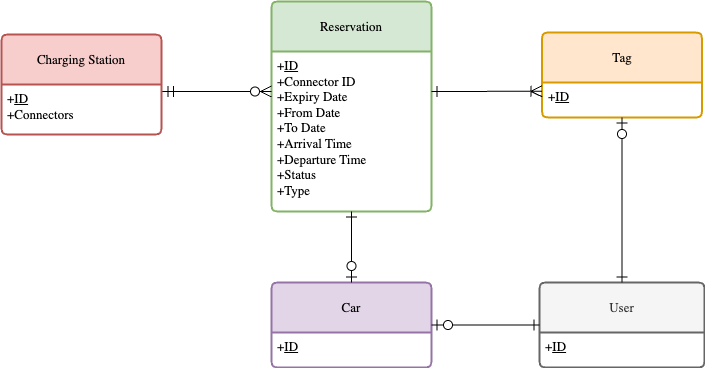
\includegraphics[scale=0.4]{resources/images/main/5_design/Entities.png}
    \caption{Entities and their relationships based on the provided scenario}
    \label{fig:entity-relationship-diagram}
\end{figure}

\section{Use Cases}
\label{ch:Design:sec:Use Cases}

To provide a basic feature set for the reservation system to work, the following use cases out of the chapter \ref{ch:Requirements Engineering} are selected. Based on this subset of features workflows are designed, the system has to implement for proper functionality.

Before implementation, the features are described and implemented using Flowchart diagrams with UML \cite{noauthor_welcome_nodate}.

\subsection{Create Reservation}
\label{ch:Design:sec:Use Cases:ssec:Create Reservation}

For creating a reservation the following steps are necessary.

\begin{figure}[!ht]
    \centering
    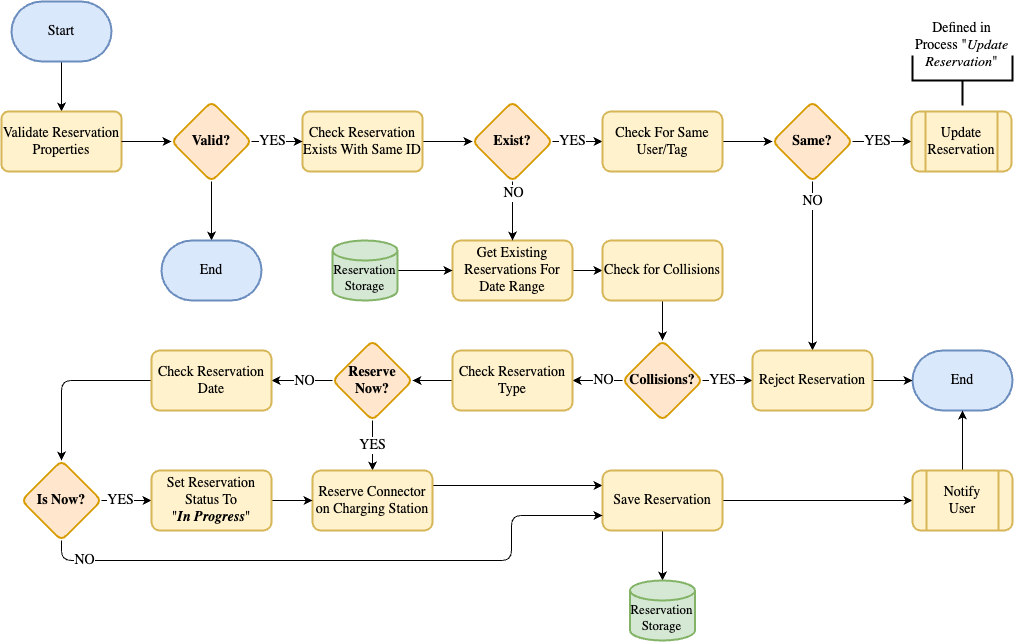
\includegraphics[scale=0.4]{resources/images/main/5_design/processes/ReservationCreate.png}
    \caption{Process flow and required steps for creating a reservation}
    \label{fig:create-reservation-flowchart}
\end{figure}

... including the design of the mockups for later implementation:

\begin{figure}
    \centering
     \begin{subfigure}[b]{0.6\textwidth}
         \centering
         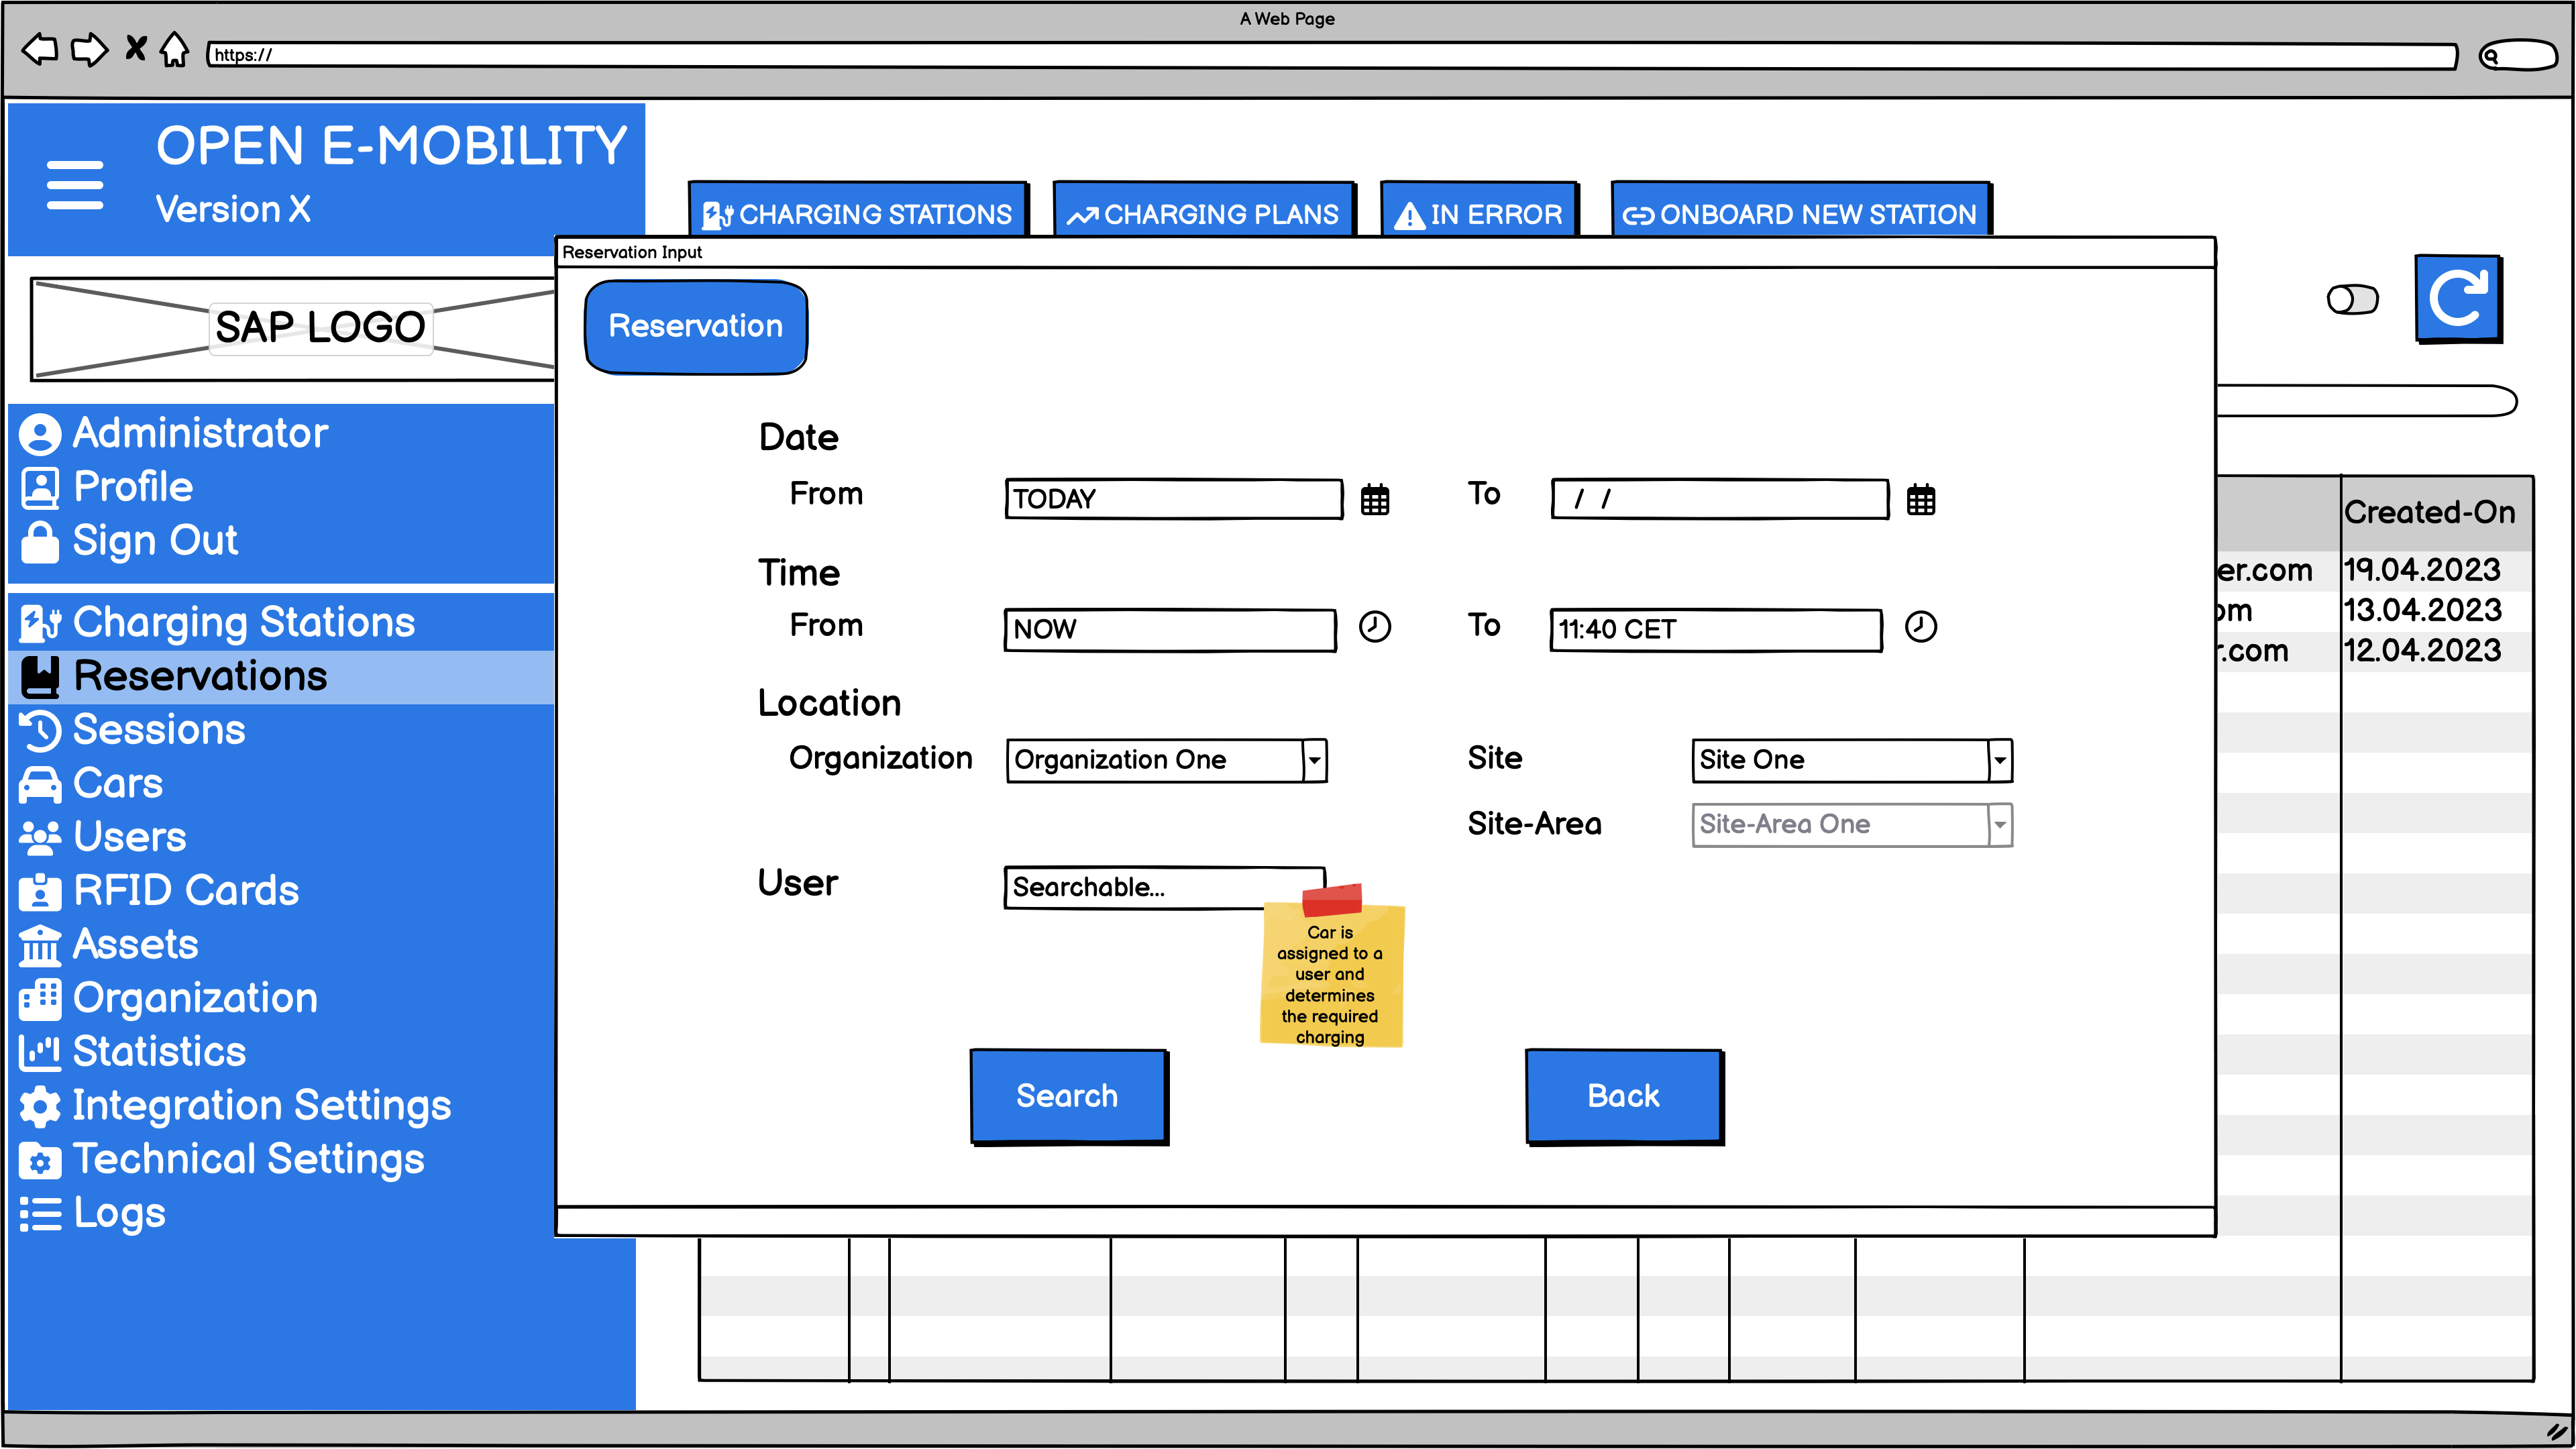
\includegraphics[width=\textwidth]{resources/images/main/5_design/mockups/create_reservation/web/1_Reservation_Create.png}
         \caption{Web Frontend}
         \label{fig:web-create-reservation}
    \end{subfigure}
     \hfill
     \begin{subfigure}[b]{0.3\textwidth}
         \centering
         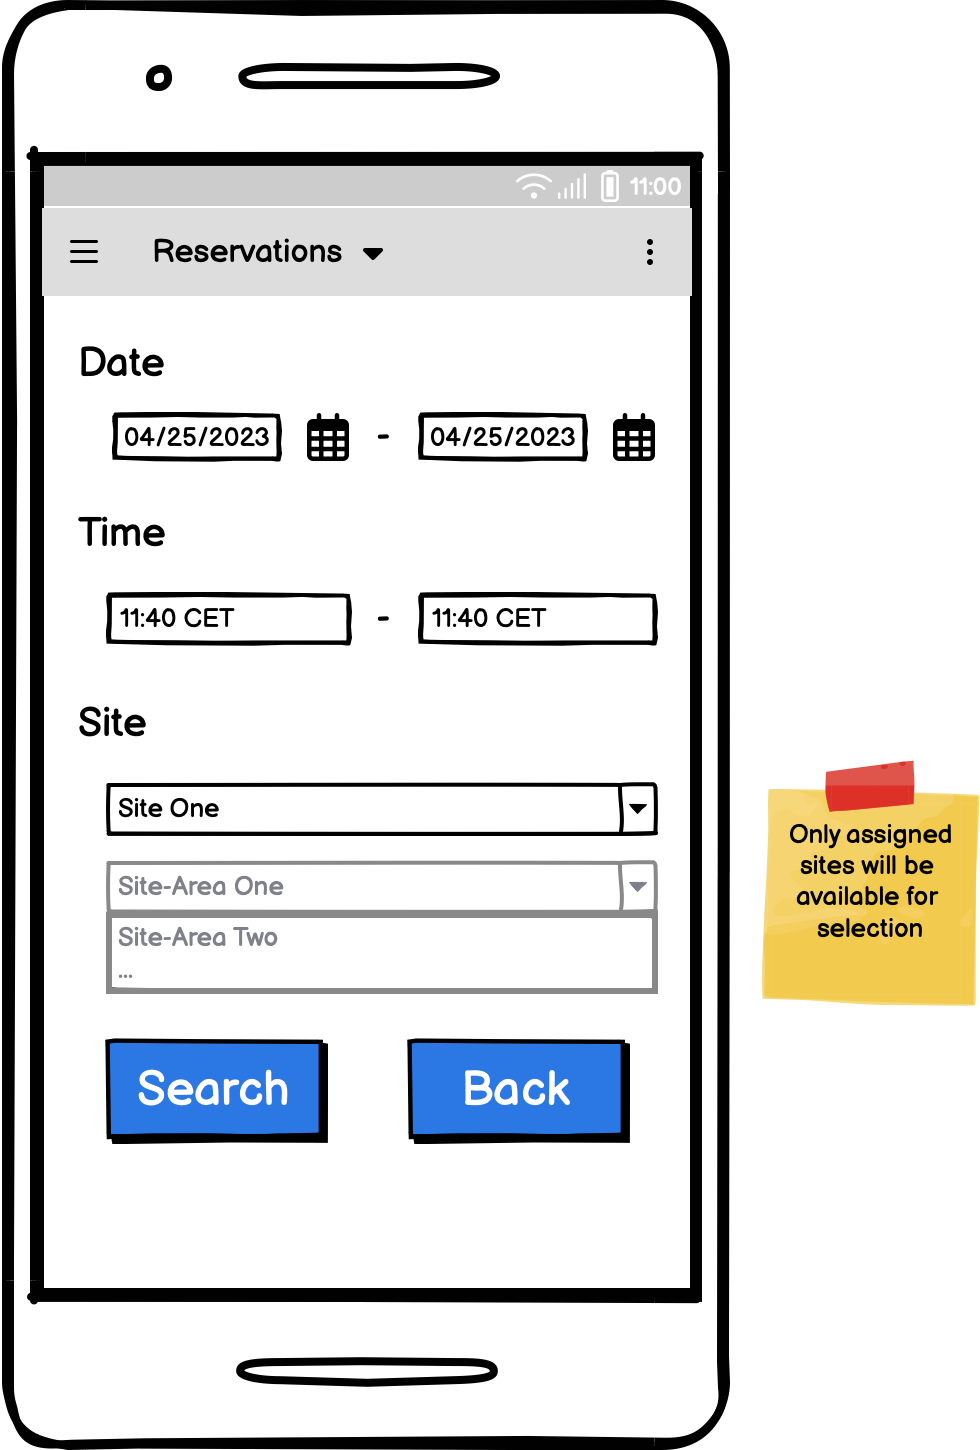
\includegraphics[width=\textwidth]{resources/images/main/5_design/mockups/create_reservation/mobile/2_Create_Reservation.png}
         \caption{Mobile}
         \label{fig:mobile-create-reservation}
    \end{subfigure}
    \caption{Comparison of mobile and web frontend regarding the creation of reservations}
    \label{fig:create-reservation-design}
\end{figure}

\subsection{Update Reservation}
\label{ch:Design:sec:Update Reservation}

For updating a reservation the following steps are necessary.

\begin{figure}[!ht]
    \centering
    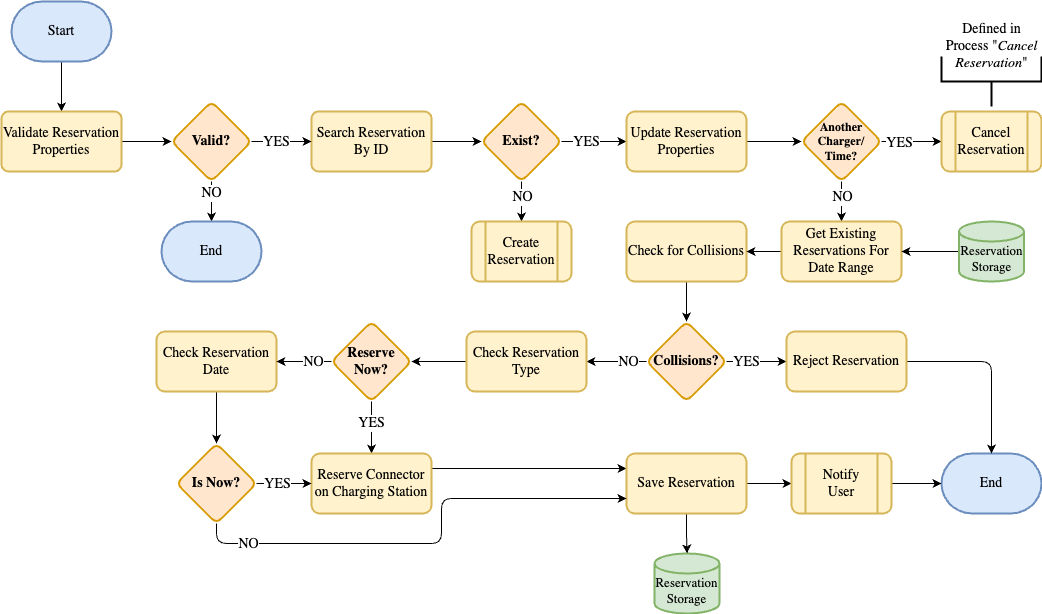
\includegraphics[scale=0.4]{resources/images/main/5_design/processes/ReservationUpdate.png}
    \caption{Process flow and required steps for updating a reservation}
    \label{fig:update-reservation-flowchart}
\end{figure}

\subsection{Delete Reservation}
\label{ch:Design:sec:Use Cases:ssec:Delete Reservation}

For deleting a reservation the following steps are necessary.

\begin{figure}[!ht]
    \centering
    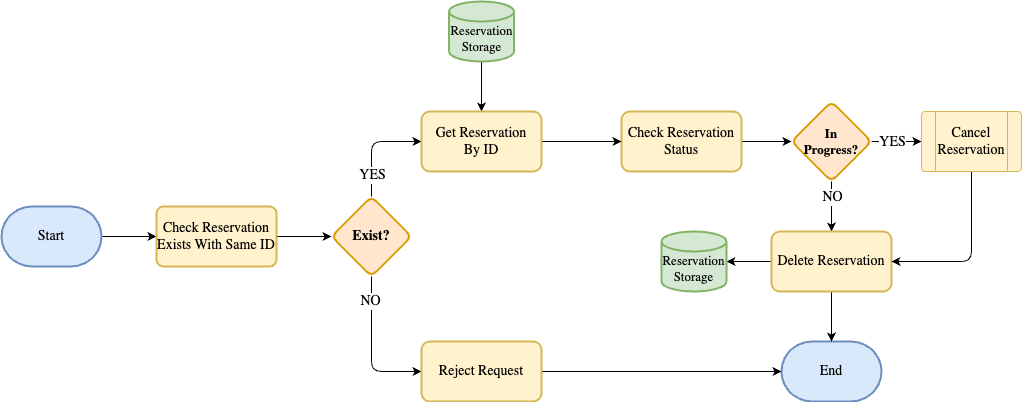
\includegraphics[scale=0.4]{resources/images/main/5_design/processes/ReservationDelete.png}
    \caption{Process flow and required steps for deleting a reservation}
    \label{fig:delete-reservation-flowchart}
\end{figure}

\subsection{Cancel Reservation}
\label{ch:Design:sec:Use Cases:ssec:Cancel Reservation}

\begin{figure}[!ht]
    \centering
    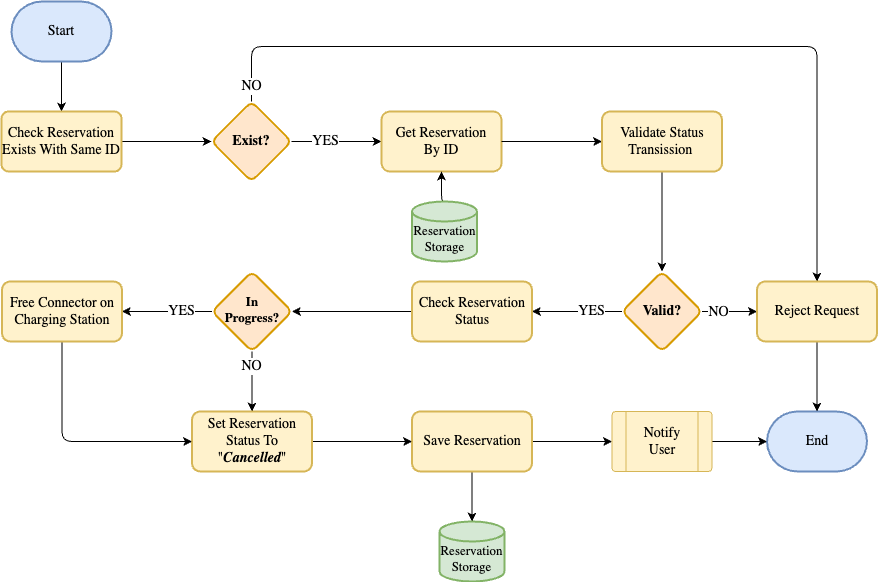
\includegraphics[scale=0.4]{resources/images/main/5_design/processes/ReservationCancel.png}
    \caption{Process flow and required steps for cancelling a reservation}
    \label{fig:cancel-reservation-flowchart}
\end{figure}

\subsection{Schedule Reservation}
\label{ch:Design:sec:Use Cases:ssec:Schedule Reservation}

\begin{figure}[!ht]
    \centering
    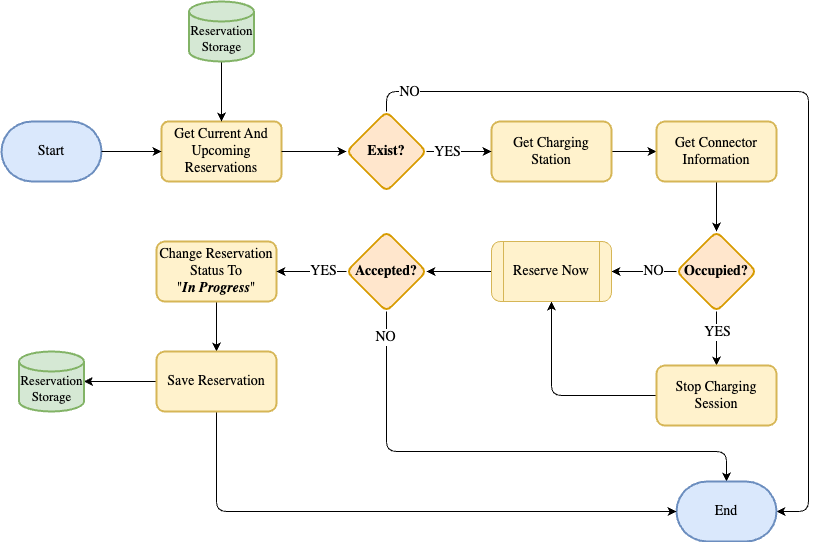
\includegraphics[scale=0.4]{resources/images/main/5_design/processes/scheduler/SynchronizeReservation.png}
    \caption{Process for scheduling upcoming reservation on the specified \acrshortpl{cs}}
    \label{fig:schedule-reservation-flowchart}
\end{figure}

\subsection{Expire Reservation}
\label{ch:Design:sec:Use Cases:ssec:Expire Reservation}

\begin{figure}[!ht]
    \centering
    
\includegraphics[scale=0.4]{resources/images/main/5_design/processes/scheduler/UpdateExpiredReservations.png}
    \caption{Process flow for reservations reaching their expiry date}
    \label{fig:expire-reservation-flowchart}
\end{figure}

\subsection{Free reserved connectors}
\label{ch:Design:sec:Use Cases:ssec:Free reserved connectors}

Afterwards the design of the process...

\begin{figure}[!ht]
    \centering
    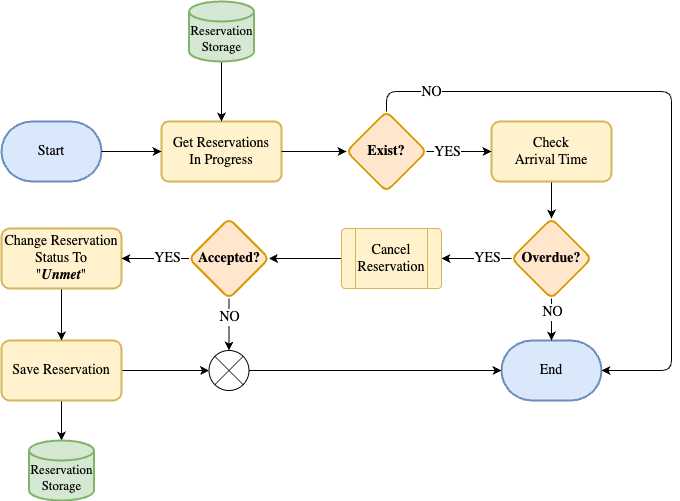
\includegraphics[scale=0.4]{resources/images/main/5_design/processes/scheduler/CancelUnmetReservation.png}
    \caption{Entities and their relationships based on the provided scenario}
    \label{fig:free-connector-flowchart}
\end{figure}

% Should include notifications descriptions in regards to 'Charging reservation service for electric vehicles using automatic notification'

% \section{Not Use Cases}
% \label{ch:Design:sec:Not Use Cases}

% \subsection{Smart Charging Integration}
% \label{ch:Design:sec:Not Use Cases:sec:Smart Charging}

%% LaTeX2e class for student theses
%% sections/main/6_implementation.tex
%%
%% Karlsruhe University of Applied Sciences
%% Faculty of Computer Science and Business Information Systems
%%
%% --------------------------------------------------------
%% | Derived from sdqthesis by Erik Burger burger@kit.edu |
%% --------------------------------------------------------

\chapter{Implementation}
\label{ch:Implementation}

To build on the design of the processes in the previous chapter, the actual implementation of the corresponding functionality within the applications of the underlying solution is presented.
First, some preliminary work is considered, using the standard functionality for reservations according to the \acrshort{ocpp} standard in version 1.6.
This foundation allows the extension to encapsulate these functionalities in order to ensure compliance with the standard.
After completing the initial development stages, the proposed design for the entities and processes is translated into code. This is succeeded by an analysis to identify the packages and components that the extension must use to ensure its operability.
Considering the system roles mentioned in Chapter \ref{ch:Requirements Engineering}, the assignment of the respective rules, the allowed scopes, and the respective functionality are taken into account.
Furthermore, to enable access through client applications, the implemented functionality is mapped to specific endpoints, representing resources according to the underlying \acrshort{rest} principles described in \ref{ch:Fundamentals:sec:Data Exchange:ssec:REST}.
A more detailed insight into these resources, in combination with their behavior, is offered at the end, highlighting the interaction between the components to satisfy the preconceived logic. \\
\noindent Concerning solely the creation and management process, emphasis is given to the development of the parts, that constitute the logical units of the process. 
While the frontend logic is vital to illustrate the user interaction with the backend service and guide them through the procedure, the corresponding implementations are only shown as the established interfaces based on the pre--existing designs in the applications.
This bridges the gap between the mockups created in terms of their influence on the final results. Hence, they are included as an attachment to each specified capability. 
The same applies to the frameworks and programming languages used. To provide a technology--agnostic approach, the specific characteristics of the technologies in terms of implementations are not addressed.
However, for reasons of completeness, the frameworks and programming languages used are noted below. \textit{Node.js} framework \cite{noauthor_nodejs_nodate} is used for the backend development and the charging station simulator, \textit{Angular} \cite{noauthor_angular_nodate} for the web frontend and \textit{React Native} \cite{noauthor_react_nodate} as a cross--platform framework for the mobile application. The preferred programming language is \textit{TypeScript} \cite{noauthor_javascript_nodate}, which serves as a type--safe extension of \textit{JavaScript} \cite{noauthor_javascript_2023}.

\section{System Prerequisites}
\label{ch:Implementation:sec:System Prerequisites}

In terms of standards compatibility, there were issues with the backend, web frontend, and mobile application, as they did not support the \textit{ReserveNow} operation of \acrshort{ocpp} version 1.6, nor did they support the \textit{Cancel Reservation} operation either.
Additionally, the \acrshort{cs} simulator used for local simulations of the test environment also lacked this functionality.
To establish a common baseline, as mentioned in Chapter \ref{ch:Approach}, the first step of the implementation phase, was to align the current implementation status with the predefined operations in the relevant standard.
As a result, the necessary entities and feature toggles were implemented and verified against the processes, outlined in the \acrshort{ocpp} standard documentation.
Not included in this study is a comprehensive explanation of the development steps, required to adjust the applications, which is assumed to be a necessary prerequisite for the topic covered in this study.
Although other standards, such as the \acrshort{ocpi} or \acrshort{oicp} mentioned in Chapter \ref{ch:Fundamentals} and part of the backend implementation, also offer reservation proposals, these are not addressed in this work as well.

\section{Reservation}
\label{ch:Implementation:sec:Reservation}

Beginning with the implementation of the proposed entity based on the given design.
To ensure type safety and to comply with the existing design of the application, using the type--safe system of \textit{TypeScript}, the entities are implemented as interfaces.
By employing this technique, this implementation ensures the specific types for their corresponding properties and considers software design principles such as reusability suggested by Gamma~et~al. in \cite[p.~47ff]{gamma_design_2015}. 
In addition to providing extensibility through the potential of deriving from these instances, this interface--driven method enables developers to adapt the entities and combine them into more complex types, covering advanced scenarios. \\
\noindent To implement the dedicated statuses and types, and to associate them with the appropriate stages in their life cycle, the concept of \textit{Enumerations} is used. This ensures secure type transitions, as suggested in the design chapter, and is widely available in most programming languages.
An example of such predefined life cycle transitions is provided by the implementation in listing \ref{listing:state-transitions}, which covers some instances of transitions below. 

\lstinputlisting[caption={State transitions enforcing the reservation life cycle using \textit{TypeScript}}, label=listing:state-transitions, language=TypeScript]{resources/code/states/state_transitions.ts}

\noindent The resulting class diagram reveals the final implementation of the classes within the codebase, which, in addition to the \texttt{Reservation} interface, includes the connections to the other parts of the resulting entity.
Alongside the previously mentioned \texttt{ReservationStatus} and the \texttt{ReservationType}, the diagram in Figure \ref{fig:reservation-class-diagram} shows the other relevant interfaces. 
For example, the \texttt{ReservationAuthorizationActions} as part of the internal privilege control system, ensuring access to specific operations and entities through \texttt{AuthorizationDefinitions} and their according \texttt{AuthorizationActions}. \\
Thus, these interfaces, along with the \texttt{CreatedUpdatedProps}, could be categorized as administrative properties, to provide uniform handling of system entities internally.

\begin{figure}[h]
    \centering
    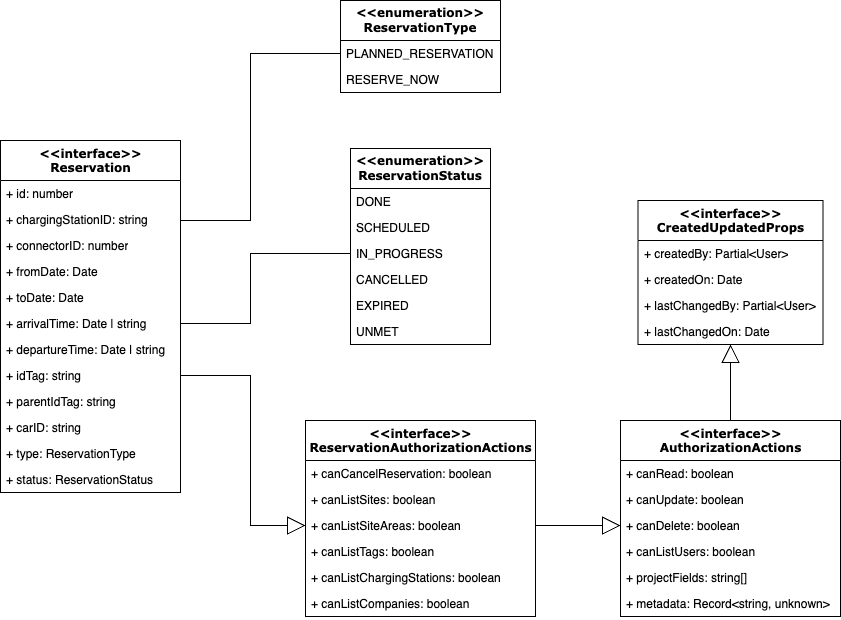
\includegraphics[width=0.8\textwidth,keepaspectratio]{resources/images/main/6_implementation/Reservation.png}
    \caption{Class diagram for the elaborated entity and its associated classes.}
    \label{fig:reservation-class-diagram}
\end{figure}

\noindent Regarding the proposed associations with the included interfaces, the resulting implementation is equivalent to the design entity relationships, shown in Figure \ref{fig:entity-relationship-diagram}, from the previous chapter. Thus, no further class diagram illustrating the quantity of each entity within the relationship is necessary in this section.
According to the \texttt{Reservation} interface as the foundation for further development, the application proposal is the next stage of this part of the thesis. 

\section{Reservation System}
\label{ch:Implementation:sec:Reservation System}

In order to take up the groundwork provided by the construction of the \texttt{Reservation} entity and the process design, the development of the reservation system according to the gathered work is next.
For a better understanding of the application serving as a baseline for the elaborated extension, the system itself is analyzed, by considering different views on the system and its modules.
As a result, different views out of the context of software architecture are used, to facilitate interested readers of this work to come up with an own implementation, utilizing the provided design approaches.

\subsection{Architectural Views}
\label{ch:Implementation:sec:Reservation System:ssec:System Architecture}

Starting with a high--level view of the existing system architecture, to identify the existing components and interfaces incorporated by the backend. 
For this reason, the module view of the backend system, shown below in Figure \ref{fig:module-view}, provides a detailed insight into the system itself, to discover the standards utilized and their associated functionalities, which are implemented as dedicated servers.
To present this highly abstract point of view, these modules are represented as functional units in terms of the decomposition style described by Clements~et al.~\cite[p.~67]{clements_documenting_2011}.
This architectural style is frequently used in order to divide the system into units of implementation that enable better structuring.
Regarding the assumptions of this work, the most significant modules and interfaces including the \acrshort{rest} server, the \textbf{WebSocket} interfaces, and the \acrshort{odata} interface, due to its growing importance in the business world and for the purpose of completeness.
In respect of the prefix used, each server responds to a different type of communication protocol to provide a specific set of features.
Enabling several clients to use the \acrshort{rest} protocol for communication purposes, the \texttt{REST Server} allows data exchange based on \acrshort{http} requests, facilitating the \acrshort{rest} principles, described in Subsection \ref{ch:Fundamentals:sec:Data Exchange:ssec:REST}. 
For this purpose, this server encloses the functionality of the subsequent servers, using so--called \acrshort{rest} resources to provide homogeneous entry points, that the clients could use to communicate with the servers behind it, without knowledge about each specific resource. 
In the case of the \textbf{WebSocket} interface, the backend system provides a reliable way to exchange data in real--time, using the \textbf{WebSocket} protocol mentioned in Subsection \ref{ch:Fundamentals:sec:Data Exchange:ssec:WebSocket}. 
Primarily, this interface is used to communicate with the managed charging infrastructure, including directly accessing the \texttt{\acrshort{ocpp} Server} for the administration of \acrshortpl{cs}.
The \texttt{\acrshort{odata} Server}, with the inclusion of the \textbf{\acrshort{odata} REST Interface}, allows \acrshort{odata} clients to access the backend functionalities. 
By enhancing the capabilities of the standard \acrshort{rest} protocol through publishing a public description of the offered services, in the form of a description document similar to the \acrshort{soap} \acrshort{wsdl}, it provides an alternative for utilizing the services in more advanced scenarios.

\begin{figure}[h]
    \centering
    \includegraphics[width=0.8\textwidth,keepaspectratio]{resources/images/main/6_implementation/DeploymentView.png}
    \caption{Overview of the various functional components within the existing project.}
    \label{fig:module-view}
\end{figure}

\noindent As indicated by Figure \ref{fig:module-view}, and due to the reliance on the targeted client applications, which primarily use \acrshort{rest} based communication, the main development work is located within the \texttt{REST server}. 
Besides its role of mapping functionality to the outside world, the corollary of integrating the reservation system inside this server is considered trivial.
For a deeper understanding of the internal structure of this server, and to reduce the architectural height to identify the relevant components and packages, for the required changes to implement the extension accordingly, the following sub--parts drill down to provide a more detailed view.

\subsubsection{Packages}
\label{ch:Implementation:sec:Reservation System:ssec:Architectural Views:sssec:Packages}

After the choice of the \texttt{REST server} as the location for the functionalities, the introduced architectural style of decomposition, allows for the arbitrary adjustment of the perspective into which a system and its modules could be further subdivided.
As part of Figure \ref{fig:package-view}, the utilized extraction process of relevant modules into packages that structure the application is displayed. This view not only shows the logical structure of the project but also allows developers to group together functionality or logical units with a high degree of cohesion in a particular location.
As introduced in the previous section with reference to the class diagram \ref{fig:reservation-class-diagram} for the reservation type, the entity, also known as a type, can be located within the \texttt{types} package. 
The \texttt{requests}, which represent pre--defined request bodies for the request \texttt{validator} instances, sanitize incoming payloads before processing. Following this naming convention, applicable to all types of implementations in the application structure, the corresponding packages could be easily identified.
So the appropriate implementations for \texttt{router} and \texttt{service}, to provide the \acrshort{rest} resources, as well as the \texttt{storage} classes for database access, can be readily determined. 
Also worth mentioning is the mapping of permissions for the existing roles within the \texttt{authorisation} package, the addition of \texttt{notification} types to notify the user, and the integration of new \texttt{tasks} to provide scheduled background jobs for autonomous reservation processing.
However, all of these artifacts and their associated changes are addressed in the following sections and are presented solely for awareness of their existence.

\begin{figure}[h]
    \centering
    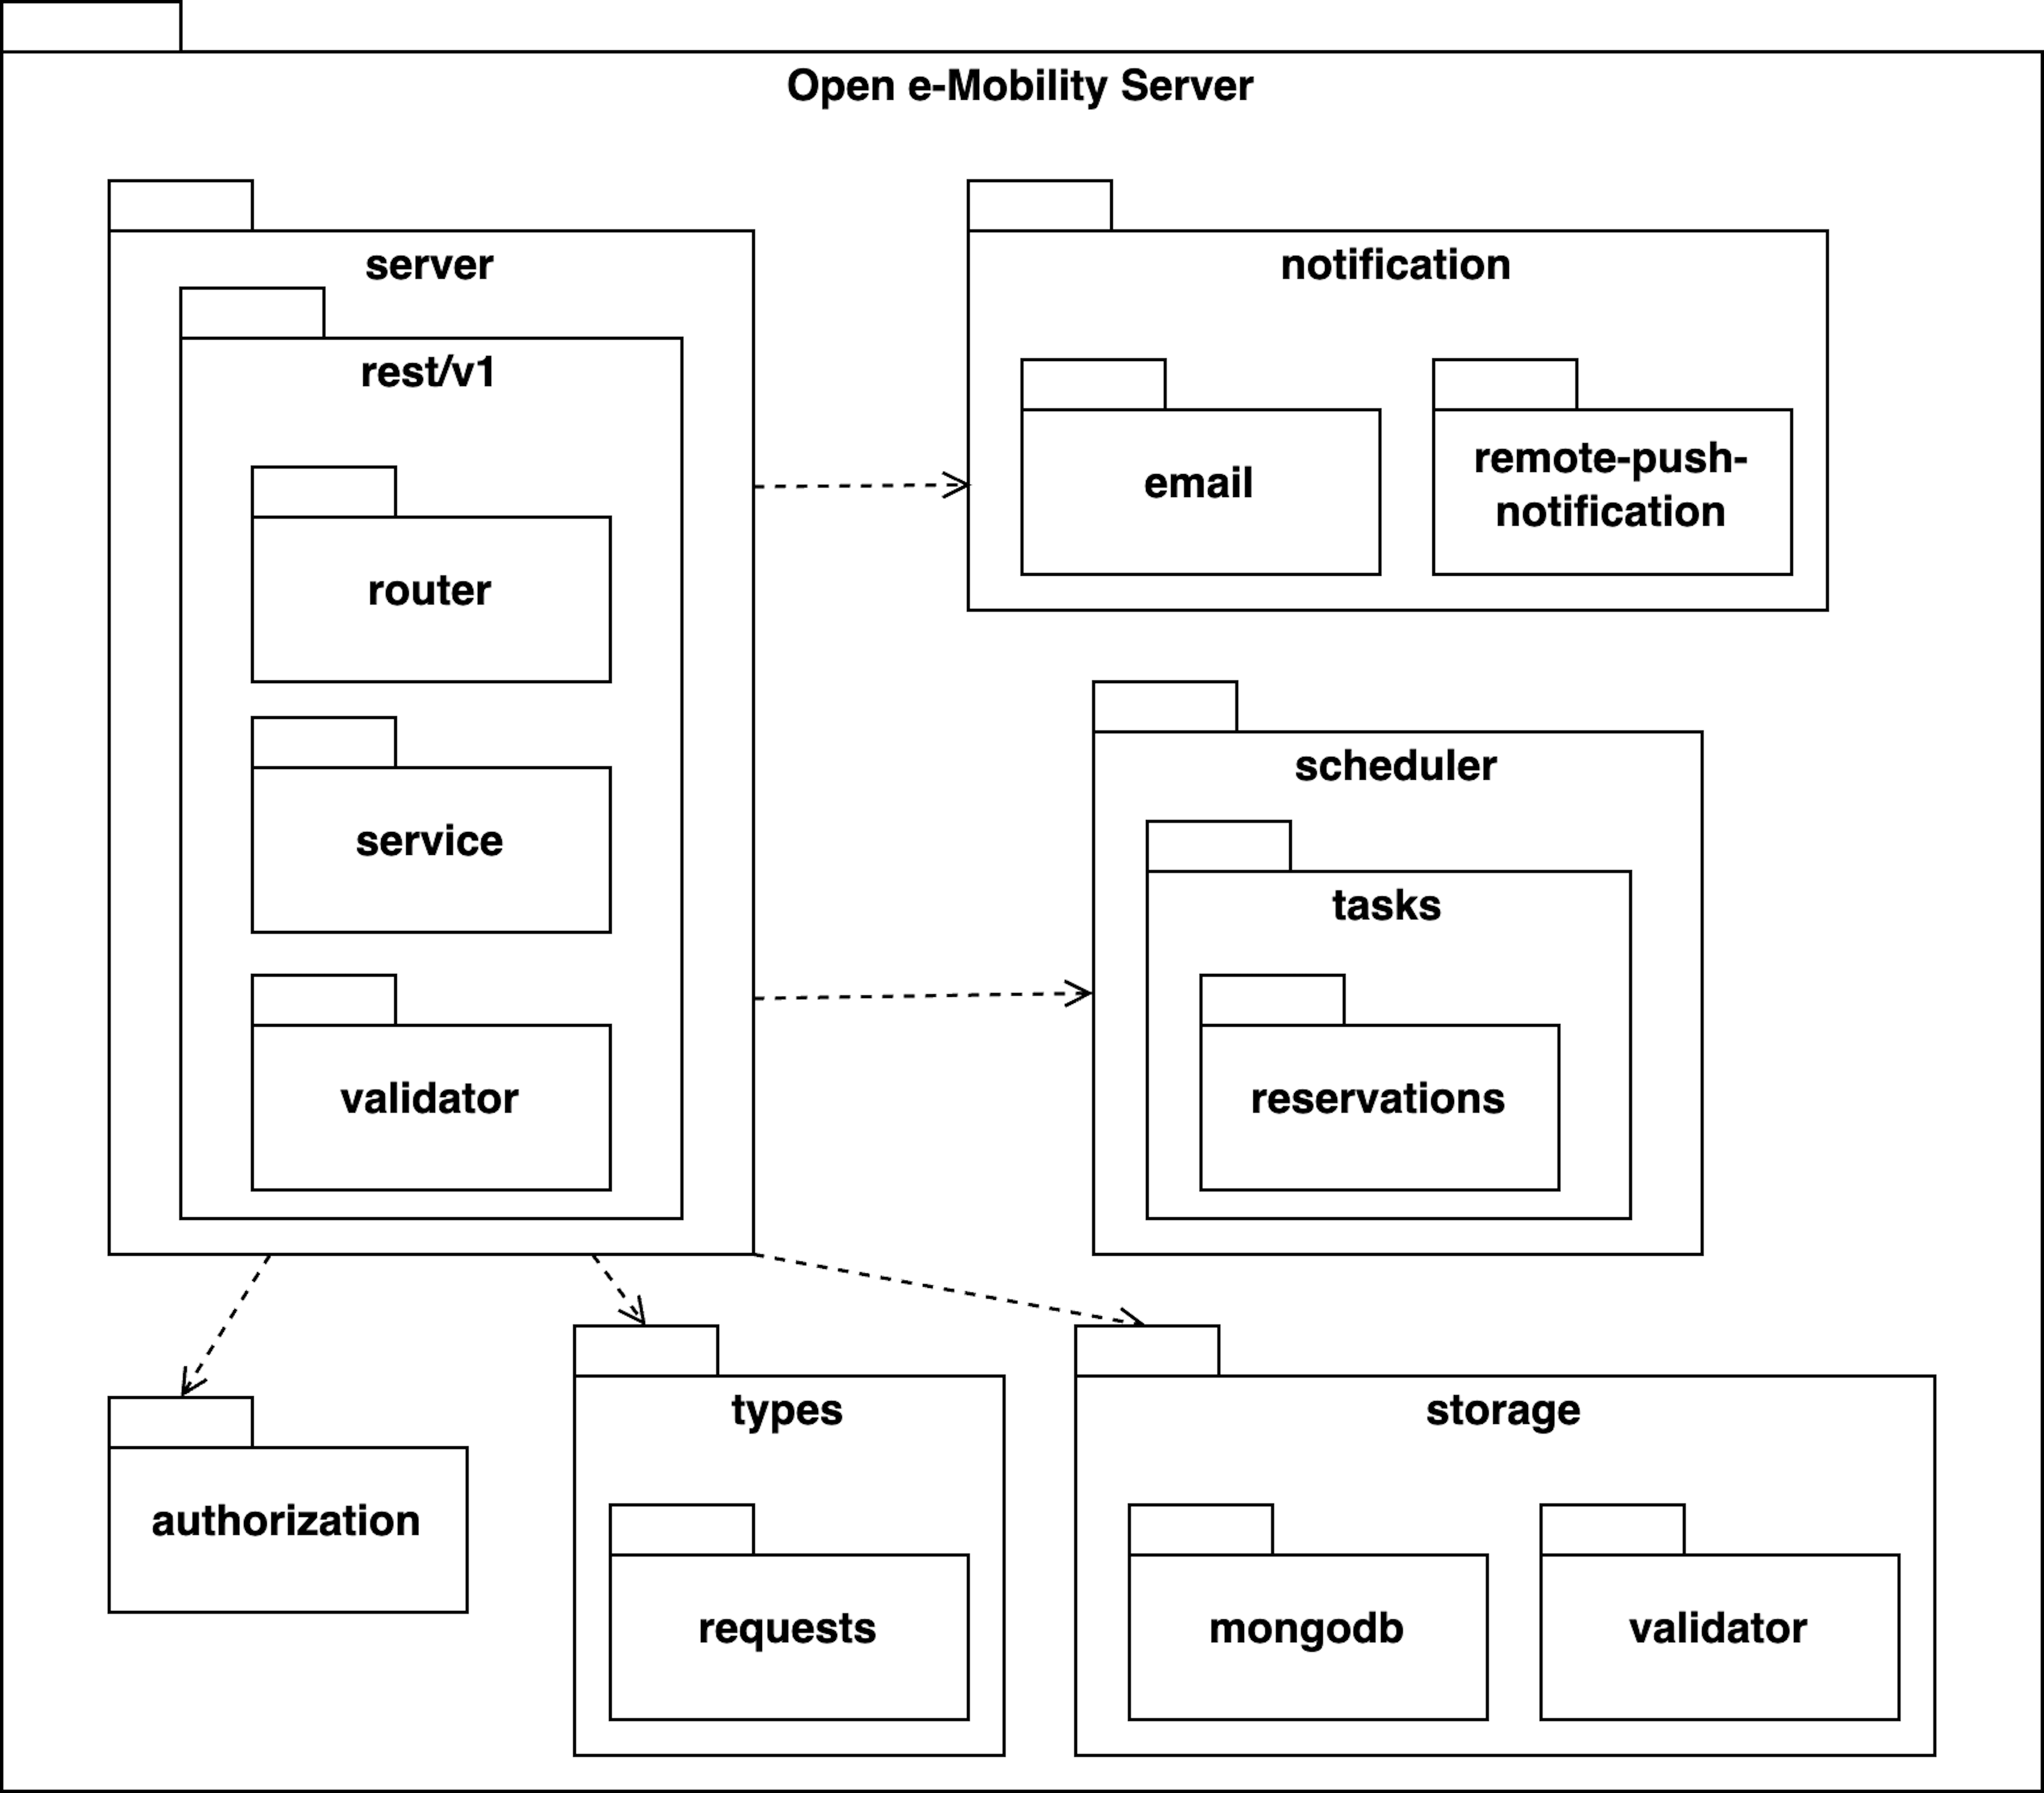
\includegraphics[width=0.8\textwidth,keepaspectratio]{resources/images/main/6_implementation/PackageDiagram.png}
    \caption{Overview of the extended packages within the targeted section of the backend project.}
    \label{fig:package-view}
\end{figure}

\noindent With the structure of the service and the location of the adaptations in mind, the next step is to introduce the components and their associated connectors. 
Architecturally, the 'component--and--connector views (C\&C)'~\cite[p.~136]{clements_documenting_2011} are used to show the inner workings of the system and the interaction between the individual components. 
Concerning the follow--up implementation, this aspect could be used for orientation and guidance in the project and provide a starting point for further development tasks, to locate the changes introduced by this work.

\subsubsection{Components}
\label{ch:Implementation:sec:Reservation System:ssec:Architectural Views:sssec:Components}

Before elaborating on the behavioral interaction between the components, all the implemented aspects have to be mapped in the context of the designed system. Thus, Figure \ref{fig:component-view} provides an overview of the added components and their integration with the already existing ones.
In line with the C\&C view, the connectors indicate the available and required functionalities and establish the appropriate connections between the corresponding components, resulting in the reservation system as part of the existing service landscape.
For the purpose of abstraction between the existing implementations and the extension, this work treats the \texttt{Reservation System} as an independent subsystem that requires only a restricted number of dependencies to other areas of the application.
Considering only the information required from other application domains, the portability as a self--contained system to other scenarios should be guaranteed.

\begin{figure}[h]
    \centering
    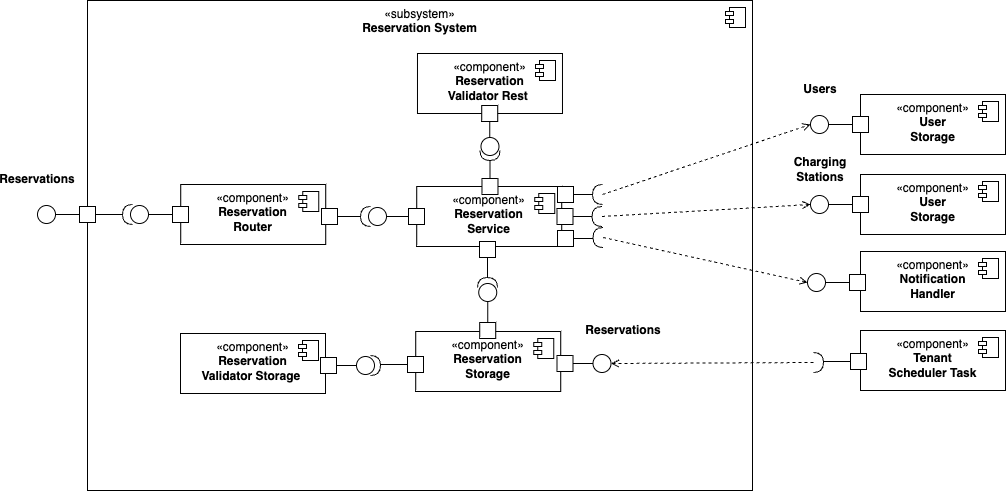
\includegraphics[width=0.8\textwidth,keepaspectratio]{resources/images/main/6_implementation/ReservationComponents.png}
    \caption{Overview of the individual components inside the extended web service.}
    \label{fig:component-view}
\end{figure}

\noindent Taking the design principles of the initial developers and the previously mentioned package structure into account, the \texttt{Reservation System} must contain several classes necessary for the \acrshort{rest}ful web service implementation.
This includes the use of a \texttt{Reservation Router} that manages incoming requests of client applications and allocates them to the relevant methods offered by the \texttt{Reservation Service}, determined by the requested resource and the parameters in the \acrshort{url}.
In the majority of cases, data is requested, which is provided by the \texttt{Reservation Storage}, encapsulating the access to the database and maintaining the lifetime of the corresponding connection.
To verify the entities arriving with the \acrshort{http} request bodies that are to be persisted in the database, the \texttt{Reservation~Validator~Rest} after receiving the requests and the \texttt{Reservation~Validator~Storage} before further processing in the database, form the first layer of validation, to prevent malformed input.
Finally, the \texttt{Notification~Handler} and the \texttt{Tenant~Scheduler~Task} represent pre--existing components utilized by the \texttt{Reservation System} for supportive purposes and are not an explicit part of the system itself.
According to its name, the \texttt{Notification Handler} is responsible for dispatching notifications to the relevant user in certain cases and the \texttt{Tenant Scheduler Task} coordinates background operations. 
By guaranteeing an entryway for external components and systems that require reservation capabilities, the \texttt{Reservation} interface, which points outside the system, allows access to the implemented functionalities inside.
On the basis of the elaborated components and their location within the architectural construct of the application, the next subsection continues to illustrate the relevant information flow and interaction to achieve the capabilities in relation to the design work.

\subsection{Management Capabilities}
\label{ch:Implementation:sec:Reservation System:ssec:Management Capabilities}

Combining the designed processes and the aforementioned architectural views, the next parts describe the actual functionality implemented within the system, while keeping the implemented components in mind.
Beginning with the management capabilities for the respective entities, which include creation, update, deletion, and cancellation offered as the basic operations offered by this functional module. This also incorporates the administrative capability to enable the reservation extension. 
In order to gain insight into the implementation of the backend logic in the frontend parts, as well as the comparison with the previously designed mockups, this theoretical perspective is complemented by the final implementation in the frontend applications of the system.

\subsubsection{Create Reservation}
\label{ch:Implementation:sec:Reservation System:ssec:Management Capabilities:sssec:Create Reservation}

Beginning with the implementation of the \textbf{Create Reservation} functionality shown in Figure \ref{fig:create-reservation-seqflow} and executed every time receiving a request for creating a reservation from an actual user at the \texttt{ReservationRouter}. 
Delegated to the \texttt{ReservationService} by calling the \texttt{handleReservationCreate} method, the \texttt{ReservationValidatorRest} immediately validates the provided input and stops the execution and the further processing of the entity by detection of malformed or erroneous properties.
In case of a successful validation and the non--existence of a record with the same \acrshort{id}, the system checks for collisions with other bookings in the selected time range to prevent overbooking of a \acrshort{cs}.
After fulfilling all the required conditions for making a reservation, the selected \acrshort{cs} is contacted in case of a \textit{ReserveNow} reservation or a scheduled booking with an upcoming timeslot, and the entity is persisted through the \texttt{ReservationStorage}, after a final validation by the \texttt{ReservationValidatorStorage}.
Considering the scenario, if a record with the same \acrshort{id} exists, this design permits the existing reservation to be updated by conformity with the deposited \acrshort{rfid} tags as well. A mismatch otherwise results in the execution being aborted to prevent another user without the required privileges from adjusting the reservation.
Finally, a confirmation notification of the successfully created arrangement is sent to the concerned user.

\begin{figure}[h]
    \centering
    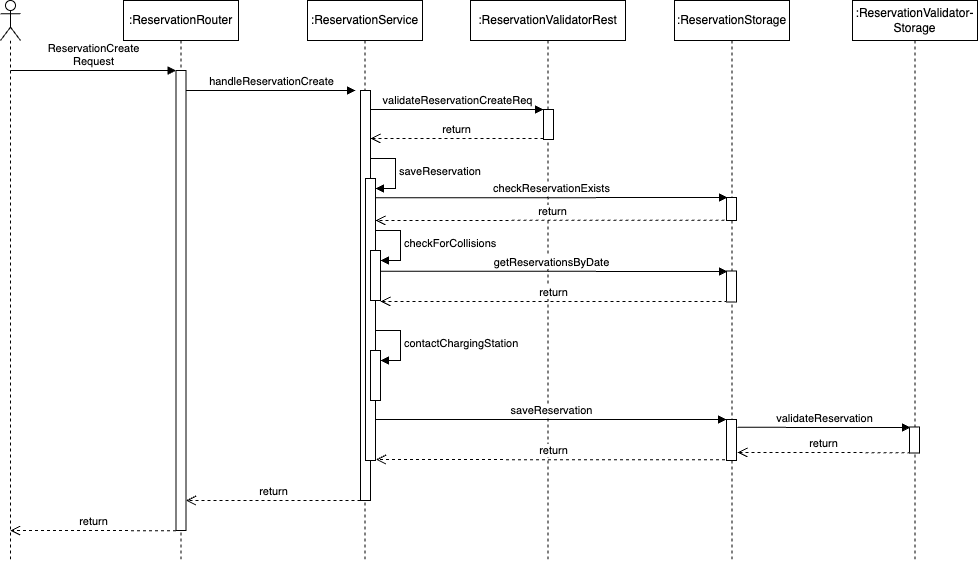
\includegraphics[width=0.8\textwidth,keepaspectratio]{resources/images/main/6_implementation/processes/ReservationCreate.png}
    \caption{Component interaction for fulfilling the process flow of creating a reservation in reference to the proposed design.}
    \label{fig:create-reservation-seqflow}
\end{figure}

\newpage

\noindent With the required booking properties in mind, the corresponding input screens of the mobile and web applications resulted in the subsequent layout shown in Figure \ref{fig:impl-create-reservation}. 
As well as mapping the relevant properties to the input fields on the user interfaces, the existing layout plays a crucial role in the proposed appearance of the result.
For supporting both types of reservations elaborated in this work, a selection toggle is implemented, which appears when the proposed extension is enabled for the respective tenant and automatically adjusts the displayed options on behalf.
In combination with an integrated validation of the input fields, the approach to provide one central interface as an entry point for creating the reservation should allow for maximum convenience for the user.
Another aspect to mention is, that the selection of a \texttt{Parent \acrshort{id} Tag}, representing a superior \acrshort{rfid} tag for a group of subordinate tags, is not considered in this particular implementation. 
This simplifies the handling of the data model and enables a one--to--one relationship between the user and the reservation.
Although the input option is absent in the frontend, the associated property indeed exists in the underlying entity.

\begin{figure}[h]
    \centering
    \begin{subfigure}[c]{0.6\textwidth}
        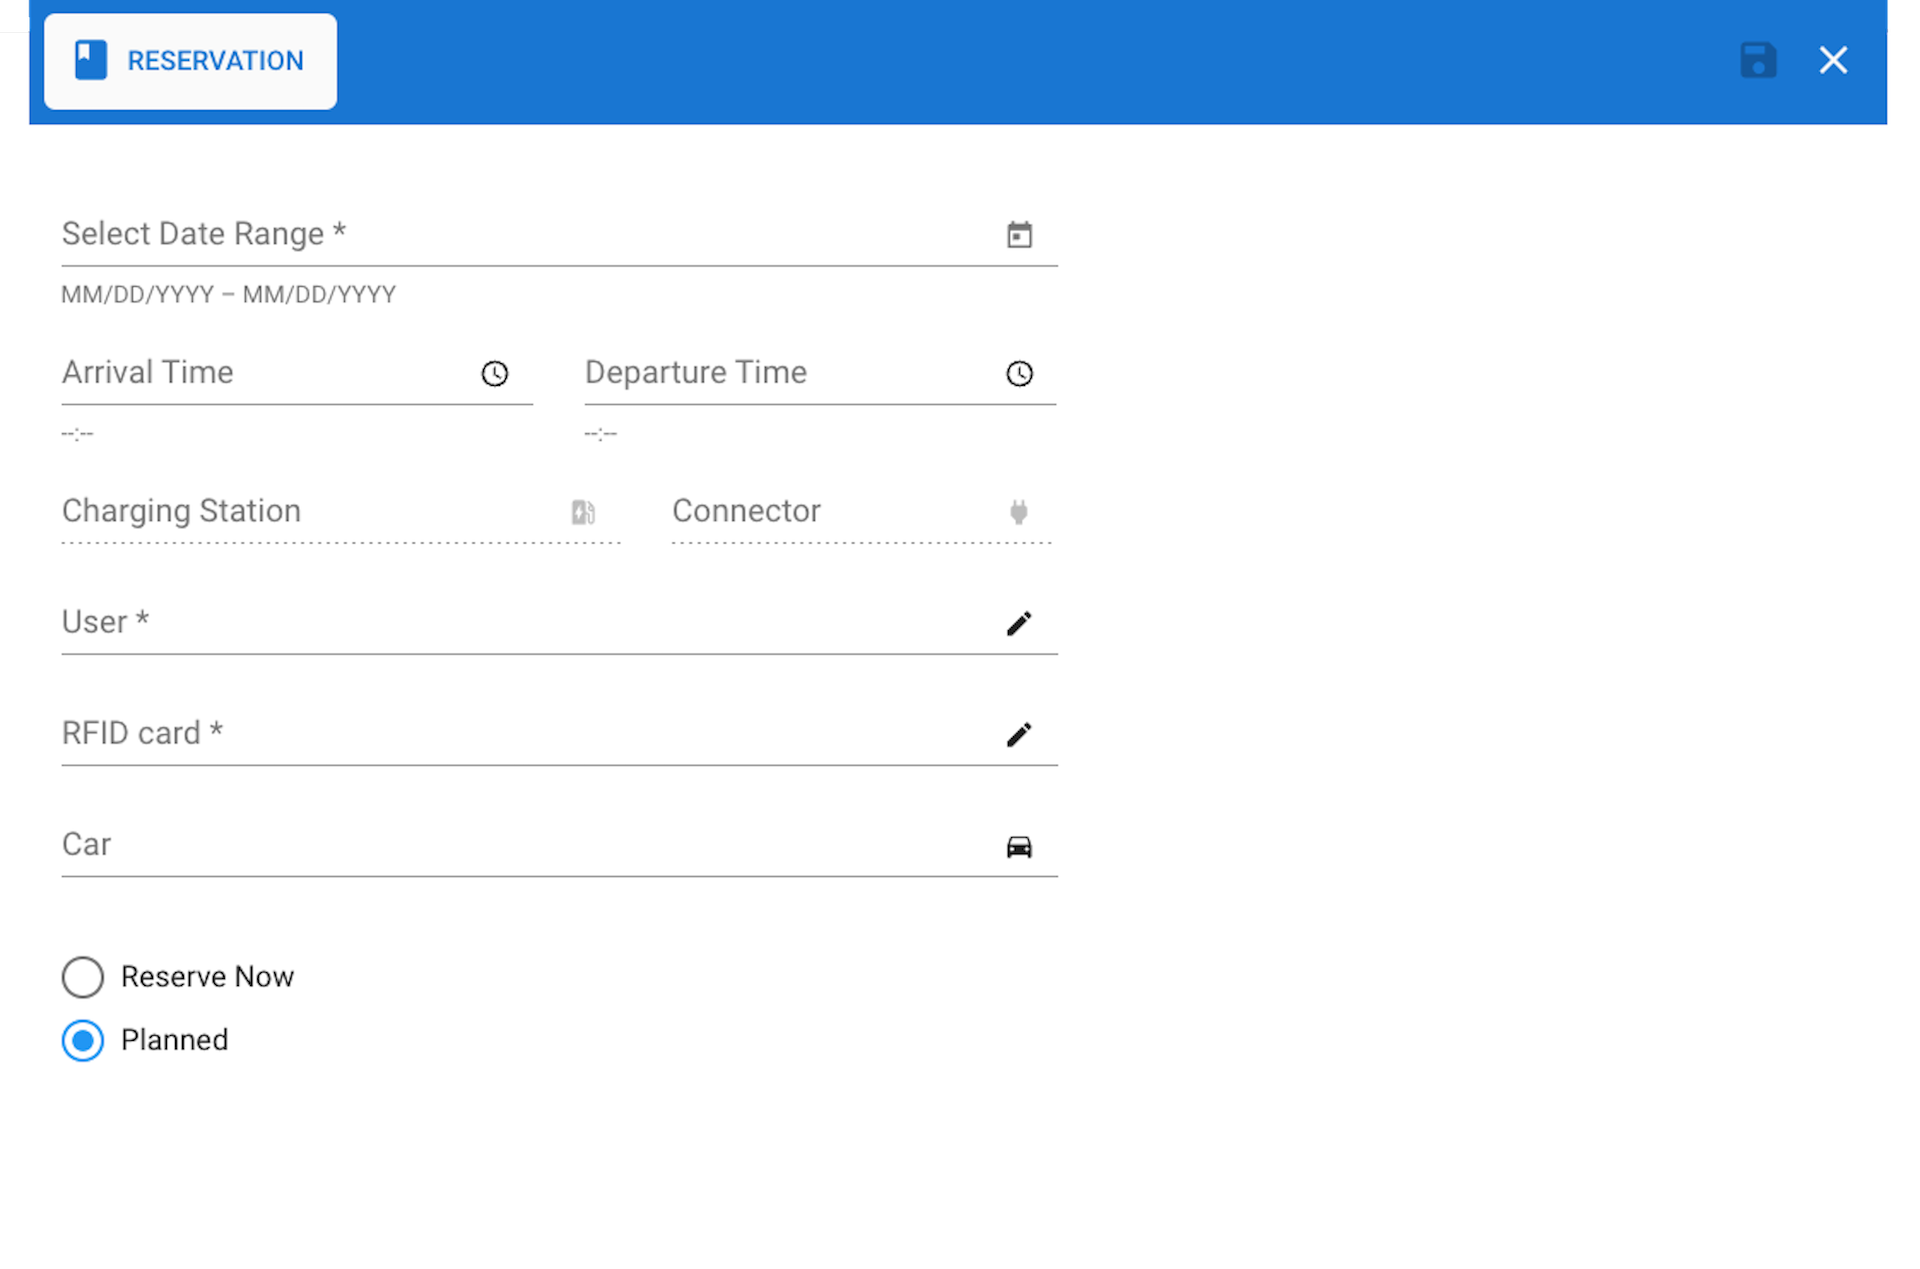
\includegraphics[width=\textwidth]{resources/images/main/6_implementation/screens/create_reservation/web/Create_Reservation.png}
        \captionsetup{skip=30pt}
        \caption{Create a reservation in the web application.}
        \label{fig:web-create-reservation-impl}
    \end{subfigure}
    \hfill
    \begin{subfigure}[c]{0.3\textwidth}
        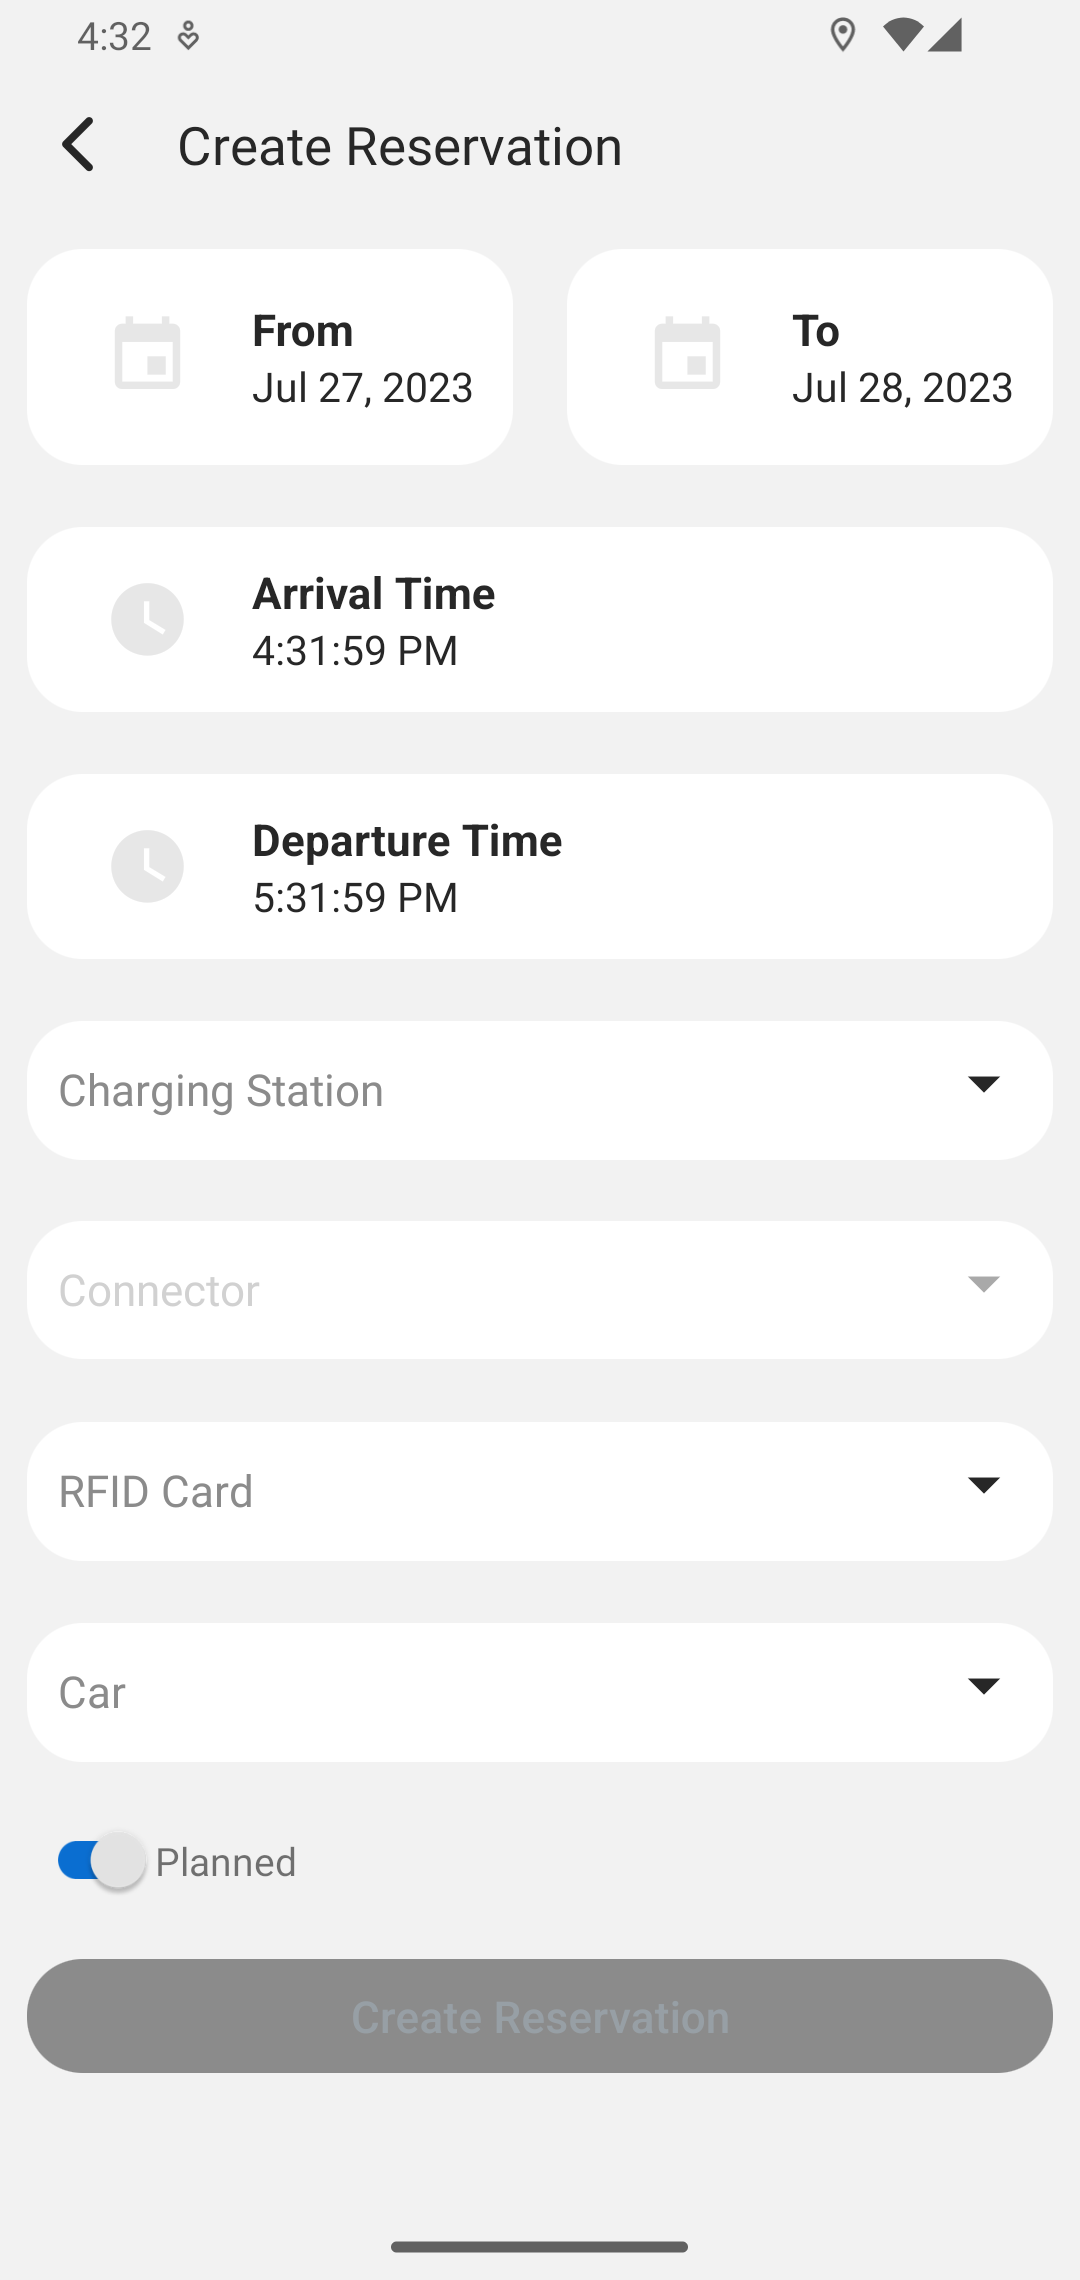
\includegraphics[width=\textwidth,height=1.6\textwidth,keepaspectratio]{resources/images/main/6_implementation/screens/create_reservation/mobile/Create_Reservation.png}
        \caption{Create a reservation in the mobile application.}
        \label{fig:mobile-create-reservation-impl}
    \end{subfigure}
    \caption{Implementation of the user interfaces of the mobile and web application relating to the creation of reservations.}
    \label{fig:impl-create-reservation}
\end{figure}

\noindent Delivering this functionality using the \acrshort{rest} methodology and the appropriate resource, the \textbf{Create Reservation} process could be called on behalf of the following endpoint listed in Table \ref{tab:create-reservation-rest}.

\begingroup
\setlength{\tabcolsep}{10pt} % Default value: 6pt
\renewcommand{\arraystretch}{1.5} % Default value: 1
\begin{table}[h]
\centering
\caption{\acrshort{rest} endpoint for reservation creation.}
    \begin{tabular}{l|c}
    Resource Identifier & HTTP Method \\ \hline
    \texttt{/reservations/} & \texttt{POST} \\    
    \end{tabular}
\label{tab:create-reservation-rest}
\end{table}
\endgroup

\newpage

\subsubsection{Update Reservation}
\label{ch:Implementation:sec:Reservation System:ssec:Management Capabilities:sssec:Update Reservation}

Despite the similarities to the previously mentioned creation process in relation to the details covered, the \textbf{Update Reservation}, pictured in Figure \ref{fig:update-reservation-seqflow}, typically expects that the arrangement the user wants to update already exists.
In conformity with its logical twin, the user request passes through \texttt{ReservationRouter} and is forwarded by the \texttt{handleReservationUpdate} method to the \texttt{ReservationService}, which implements the required update logic.
Then, \texttt{ReservationValidatorRest} performs the initial input validation, before querying the reservation associated with the provided \acrshort{id} through \\ \texttt{ReservationStorage}.
Because of the aforementioned overlaps between the creation and updating process, no further description of the other steps undertaken is given in order to avoid repetition, which results from the fact that the system updates reservations in a manner, comparable to the \acrshort{cs} outlined in the \acrshort{ocpp} standard.
As indicated there, an existing entity with the same \acrshort{id} is replaced by any incoming \textit{ReserveNow} request with the same \acrshort{id}.  
Such a flawed design could allow the cancellation of reservations made by other users, who have the same \acrshort{id} as the existing object at the station, which should be prevented. So, the proposed system approach implements a check for this uncommon but potential scenario.
Relating to future work, this behavior should be observed, as it is still included in the latest \acrshort{ocpp} version 2.0 specification.
In order to handle alterations to the \acrshort{cs} or connector, the updating procedure guarantees the revocation of the booking at the previous station and gets in contact with the new station accordingly.

\newpage

\begin{figure}[h]
    \centering
    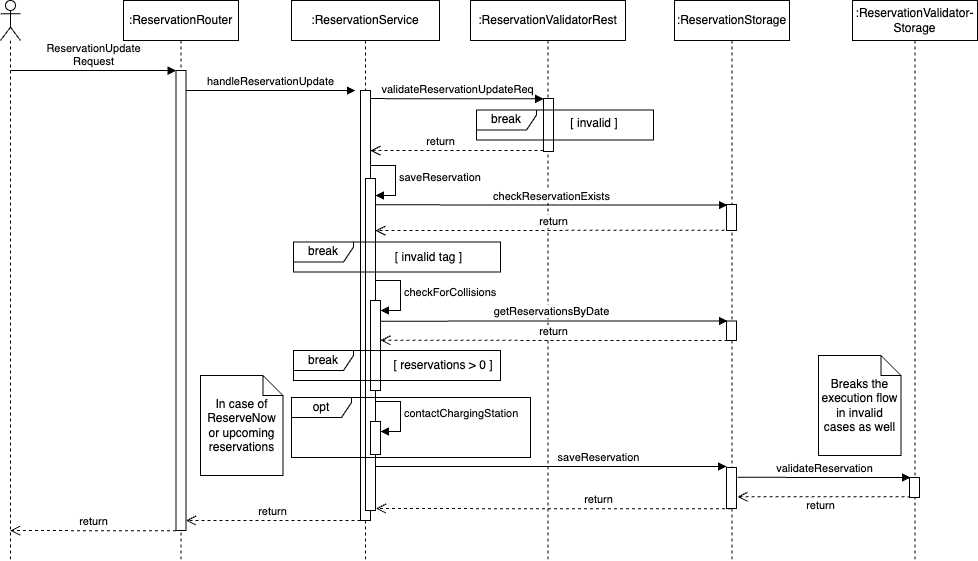
\includegraphics[width=0.8\textwidth,keepaspectratio]{resources/images/main/6_implementation/processes/ReservationUpdate.png}
    \caption{Component interaction for updating a reservation considering the proposed design draft.}
    \label{fig:update-reservation-seqflow}
\end{figure}

\noindent Because of the parallels in the underlying process, the interfaces for facilitating the update of an entity, include the same input choices as the interface designed for creation.
The sole variation within the browser application is the ability to cancel the booking within the update mask using the auxiliary \textbf{Cancel Reservation} button shown in \ref{fig:web-update-reservation-impl}. 
This feature has not been integrated into the mobile app for reasons of limited screen space and to minimize the amount of information displayed to avoid cluttered screens.

\begin{figure}[h]
    \centering
     \begin{subfigure}[c]{0.6\textwidth}
         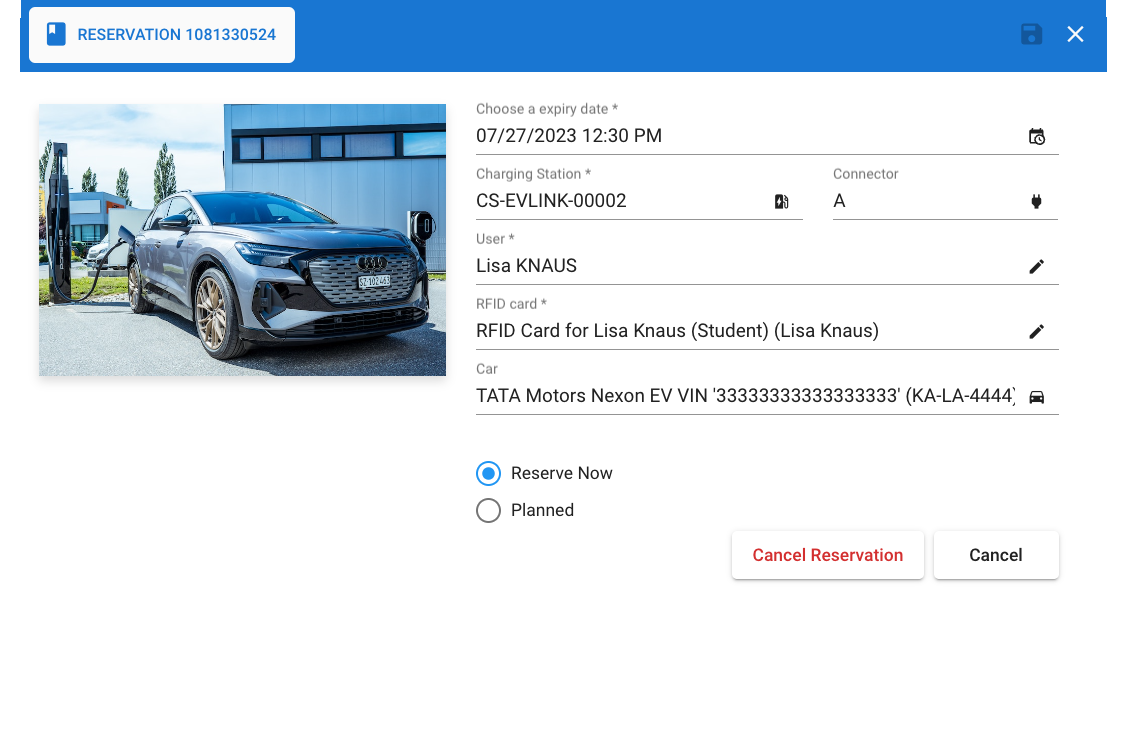
\includegraphics[width=\textwidth]{resources/images/main/6_implementation/screens/update_reservation/web/Update_Reservation.png}
         \captionsetup{skip=33pt}
         \caption{Update a reservation in the web application.}
         \label{fig:web-update-reservation-impl}
    \end{subfigure}
     \hfill
     \begin{subfigure}[c]{0.3\textwidth}
         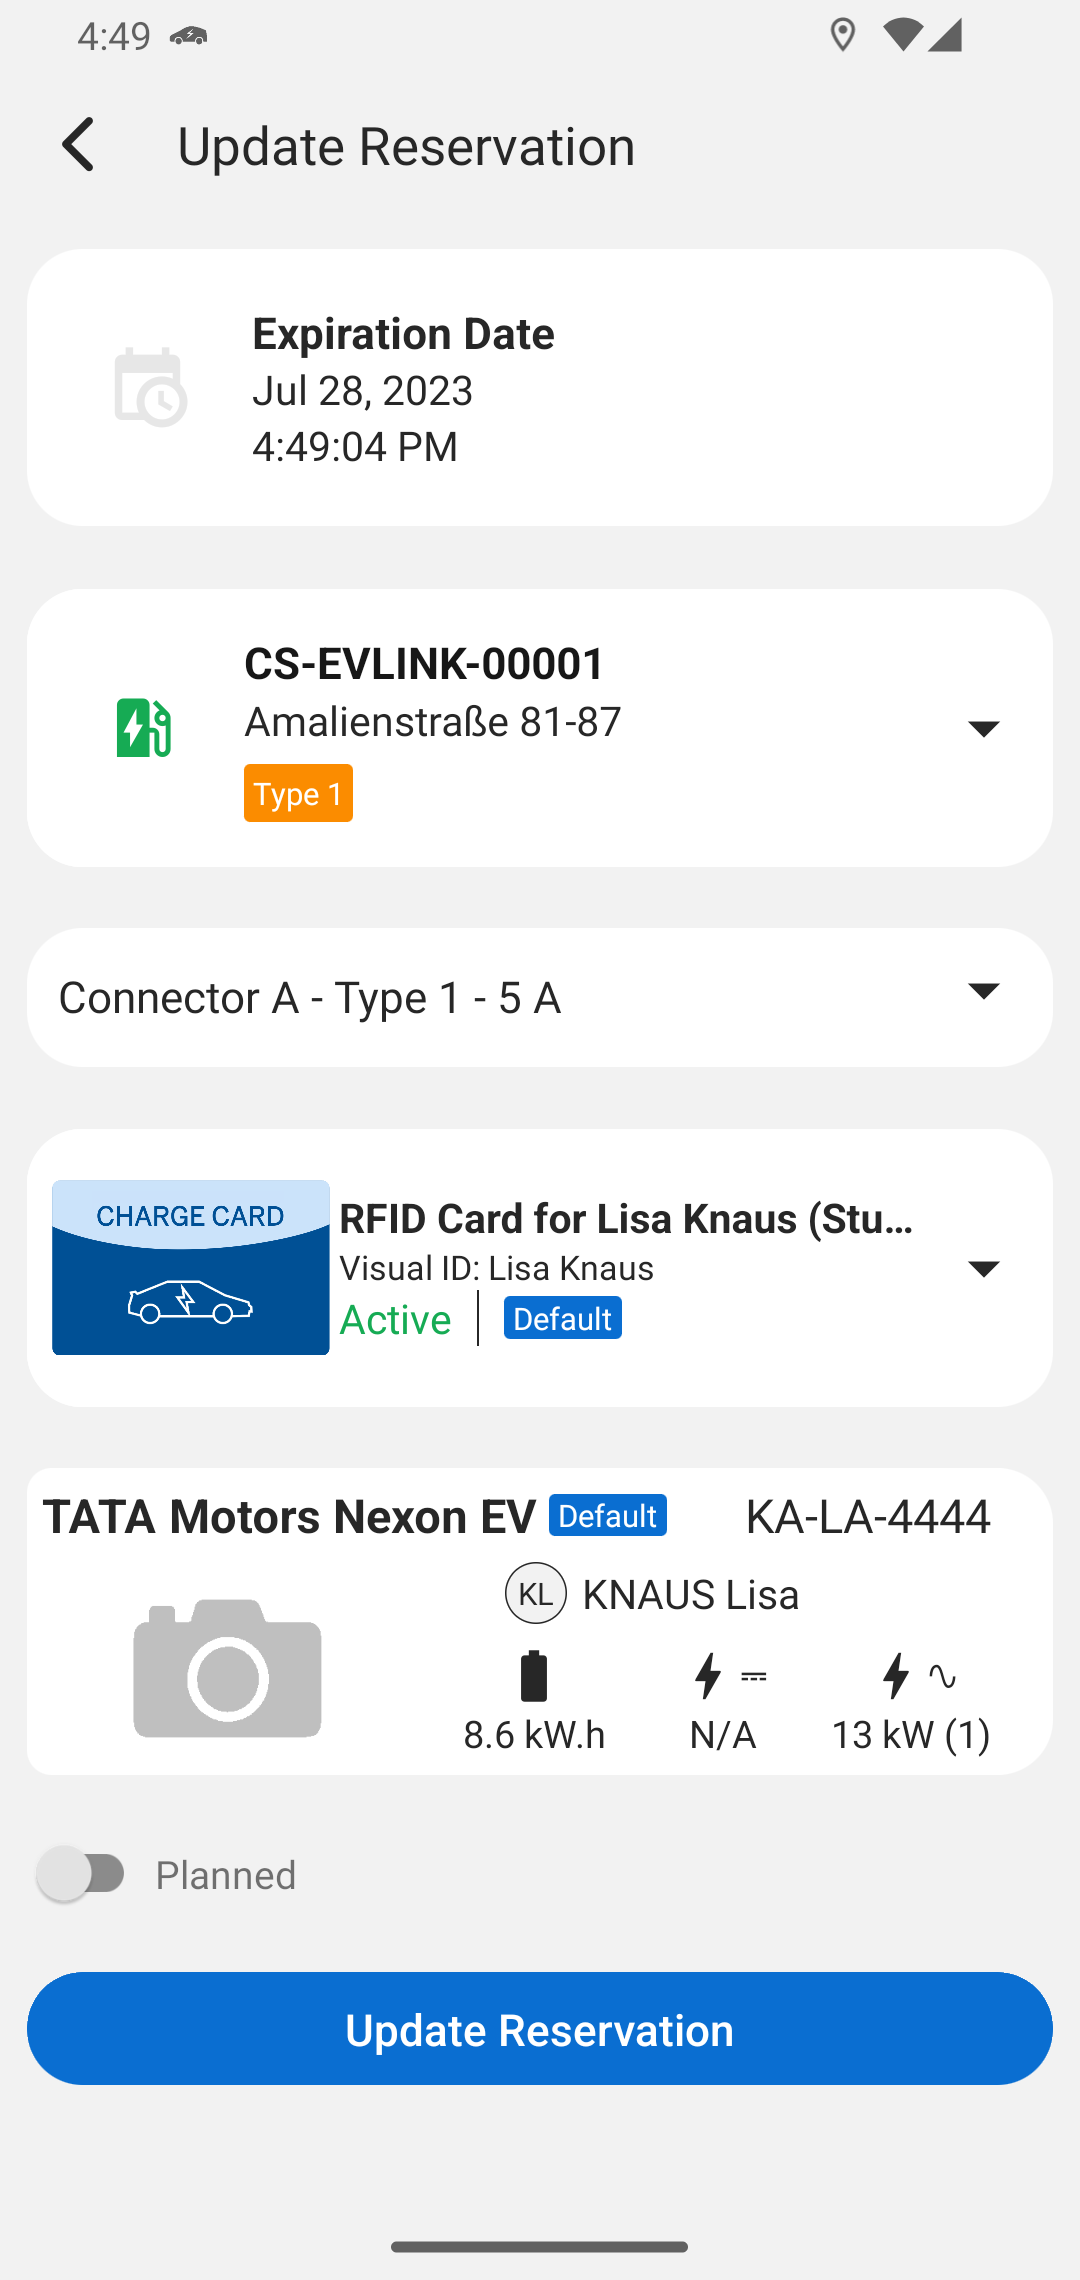
\includegraphics[width=\textwidth,height=1.6\textwidth,keepaspectratio]{resources/images/main/6_implementation/screens/update_reservation/mobile/Update_Reservation.png}
         \caption{Update a reservation in the mobile application.}
         \label{fig:mobile-update-reservation-impl}
    \end{subfigure}
    \caption{Implementation of the user interfaces of the mobile and web applications to update a reservation.}
    \label{fig:impl-update-reservation}
\end{figure}

\noindent For the interaction with the relevant client apps, the \textbf{Update Reservation} process could be called on behalf of the following \acrshort{rest} interfaces listed in Table \ref{tab:update-reservation-rest}.

\begingroup
\setlength{\tabcolsep}{10pt} % Default value: 6pt
\renewcommand{\arraystretch}{1.5} % Default value: 1
\begin{table}[h]
\centering
\caption{\acrshort{url} with path parameter for initiating an update using the respective \acrshort{rest} resource.}
    \begin{tabular}{l|c}
    Resource Identifier & HTTP Method \\ \hline
    \texttt{/reservations/\{id\}} & \texttt{PUT}
    \end{tabular}
\label{tab:update-reservation-rest}
\end{table}
\endgroup

\newpage

\subsubsection{Cancel Reservation}
\label{ch:Implementation:sec:Reservation System:ssec:Management Capabilities:sssec:Cancel Reservation}

Derived from the \textbf{Update Reservation} procedure described in \ref{ch:Implementation:sec:Reservation System:ssec:Management Capabilities:sssec:Update Reservation}, the \textbf{Cancel Reservation} operation enables the requestor, the revocation of a scheduled or already ongoing arrangement as illustrated in Figure \ref{fig:cancel-reservation-seqflow}.
Like its predecessors, the initiation of the downstream logic in the \texttt{ReservationService} undergoes the initial validation checks after request delegation by the \texttt{ReservationRouter}.
This ensures, that the incoming inquiry aligns according to the defined criteria within the solution and mitigates unintentional behavior, resulting from malformed user input.
By not ending the process prematurely due to erroneous data, the actual cancellation functionality within the service method \texttt{cancelReservation} is initiated.
Starting with the retrieval of the record from the database using the provided \acrshort{id}, the validation of the life cycle transition of the current status, as discussed in \ref{ch:Design:sec:Reservation:ssec:Reservation Status}, follows.
This ensures that only those objects that are suitable for cancellation, can be cancelled by the user and the system, otherwise, the process is terminated.
If the scheduled arrival time is already reached, the corresponding \acrshort{cs} is contacted, resulting in an immediate cancellation at that station.
After updating the status to \texttt{Cancelled}, in the case of a cancelled reservation, and successfully validating it once more, the entity is saved to the database again. The act of withdrawing a booking concludes with an outgoing cancellation notification from the \texttt{NotificationHandler} to the appropriate system user.

\newpage

\begin{figure}[h]
    \centering
    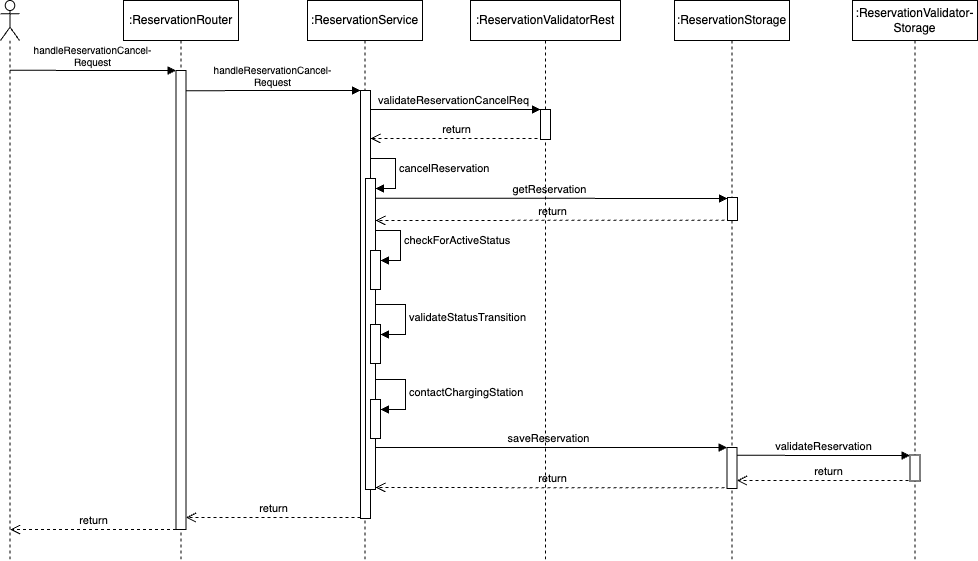
\includegraphics[width=0.8\textwidth,keepaspectratio]{resources/images/main/6_implementation/processes/ReservationCancel.png}
    \caption{The engagement of the different components during the cancellation of a reservation as proposed in the design.}
    \label{fig:cancel-reservation-seqflow}
\end{figure}

\noindent In terms of its impact on the entity and its existence within the application life cycle, the deletion of a reservation is more invasive than cancellation, which represents a practically identical atomic function, that could be realized through one single button. 
This thought led to the conclusion that such a button should be placed on each booking item on the relevant screen. Accordingly, these buttons should indicate that pressing them results in the associated cancellation of that particular booking.
In contrast to the mobile app, the webpage version permits the possibility of withdrawing already within the list overview. Enabling the user to interact more quickly with the appropriate entities, based on their current role and the assigned sites.
An example of the list view with the quick action buttons displayed at the list item level is shown in Figure \ref{fig:web-cancel-reservation-impl}, including an indicator pointing to the relevant button.

\begin{figure}[h]
    \centering
    \begin{subfigure}[c]{0.6\textwidth}
        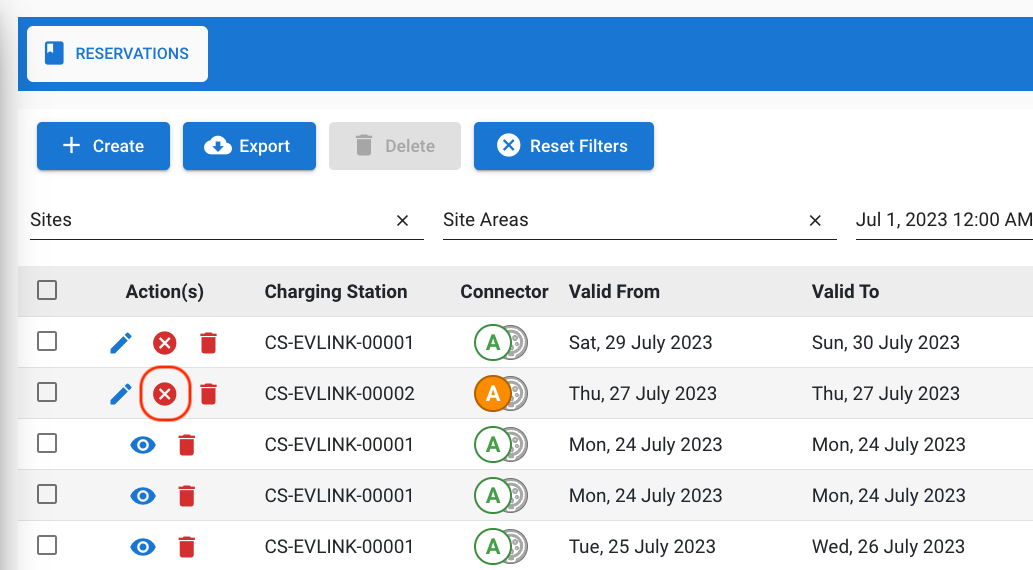
\includegraphics[width=\textwidth]{resources/images/main/6_implementation/screens/cancel_reservation/web/Cancel_Reservation.png}
        \captionsetup{skip=43pt}
        \caption{Cancel a reservation in the browser version of the app by using the \faIcon[solid]{times-circle} icon.}
        \label{fig:web-cancel-reservation-impl}
    \end{subfigure}
    \hfill
    \begin{subfigure}[c]{0.3\textwidth}
        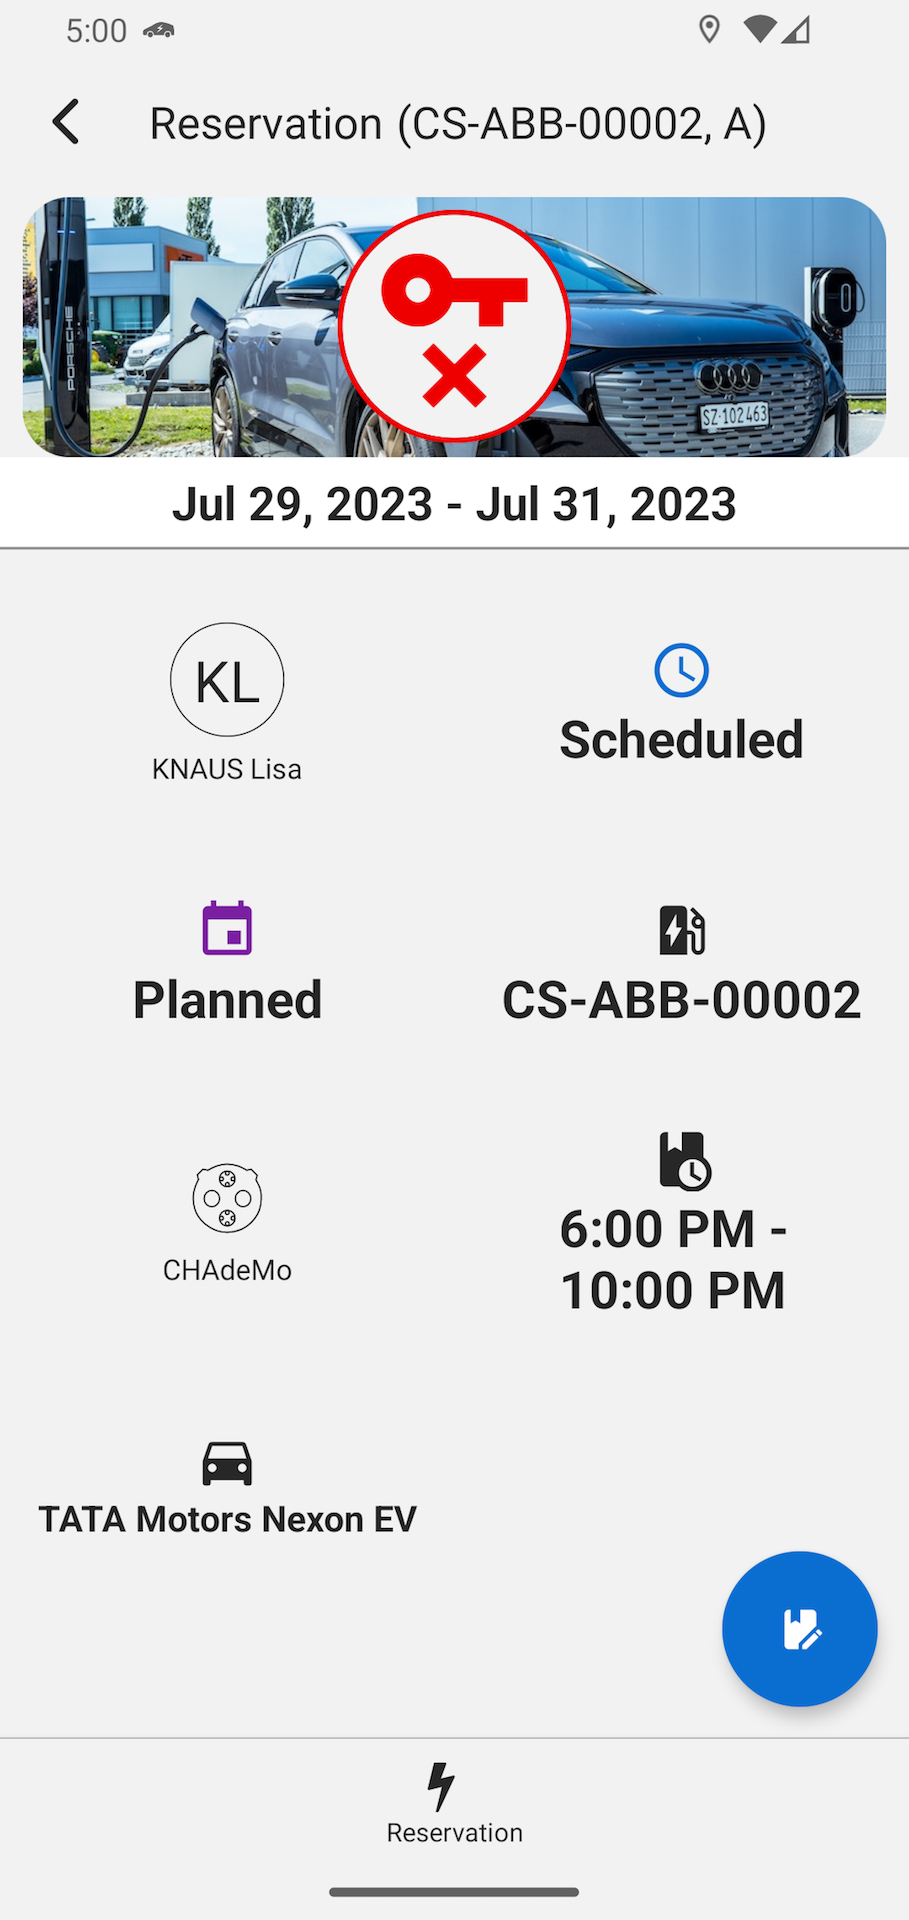
\includegraphics[width=\textwidth,height=1.6\textwidth,keepaspectratio]{resources/images/main/6_implementation/screens/cancel_reservation/mobile/Cancel_Reservation.png}
        \caption{Cancel a reservation on the mobile version from the details view of the booking.}
        \label{fig:mobile-cancel-reservation-impl}
    \end{subfigure}
    \caption{Implementation of the user interfaces of the mobile and web versions relating to the cancellation operation.}
    \label{fig:impl-cancel-reservation}
\end{figure}

\noindent To mark a booking for revocation, the related functionality could be executed using the \acrshort{rest} methodology on behalf of the following endpoint in combination with the matching \acrshort{id} as a path parameter in the \acrshort{url}.

\begingroup
\setlength{\tabcolsep}{10pt} % Default value: 6pt
\renewcommand{\arraystretch}{1.5} % Default value: 1
\begin{table}[h]
\centering
\caption{Provided \acrshort{rest} endpoints.}
    \begin{tabular}{l|c}
    Resource Identifier & HTTP Method \\ \hline
    \texttt{/reservations/\{id\}/cancel} & \texttt{PUT}
    \end{tabular}
\label{tab:cancel-reservation-rest}
\end{table}
\endgroup

\newpage

\subsubsection{Delete Reservation}
\label{ch:Implementation:sec:Reservation System:ssec:Management Capabilities:sssec:Delete Reservation}

Extending the \textbf{Cancel Reservation} functionality, \textbf{Delete Reservation} not only cancels the reservations that are currently ongoing within the system or the \acrshortpl{cs}, it also removes them from the database entirely.
As depicted in Figure \ref{fig:delete-reservation-seqflow}, when a deletion request is received from the user at the \texttt{ReservationRouter}, the \texttt{ReservationValidatorRest} validates it again and returns the process execution to the \texttt{ReservationService}. The latter continues the deletion process, once the data entered is correctly validated.
With respect to the attached \acrshort{id}, that denotes the booking the user intends to delete, the \texttt{ReservationStorage} retrieves the entity from the database and thus verifies its existence this way.
In addition to verifying the existence of the record, the current booking status is assessed to initiate additional measures for managing ongoing reservations.
This includes preventing the deletion of bookings in progress without notice, for example. To manage ongoing appointments, the system contacts the relevant stations by using the \texttt{contactChargingStation} method to release the respective \acrshortpl{cs} and connectors.
Due to the lack of a specific delete operation in the \acrshort{ocpp} standard, the deletion encapsulates the cancellation operation for a standardized communication with the \acrshort{cs}. 
As the station does not possess the ability to store history, the cancellation could be described as equivalent to a deletion at the charging infrastructure level.
After resolving the dependencies of the booking with the infrastructure, the \texttt{ReservationStorage} ultimately deletes the record in the database.

\newpage

\begin{figure}[h]
    \centering
    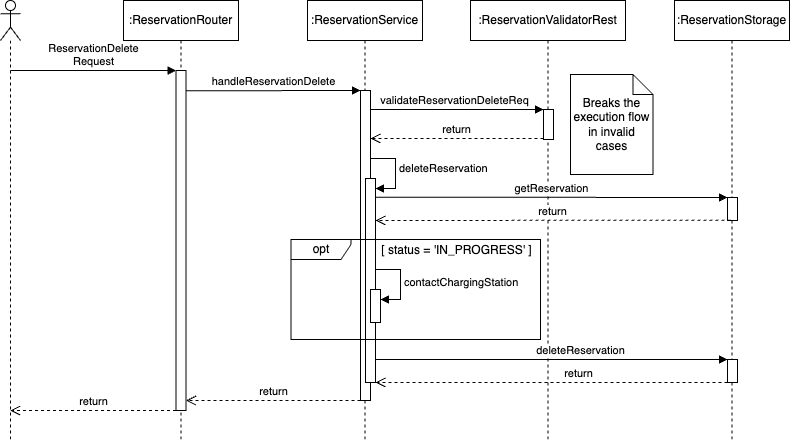
\includegraphics[width=0.8\textwidth,keepaspectratio]{resources/images/main/6_implementation/processes/ReservationDelete.png}
    \caption{Component interaction when deleting a reservation record considering the design drafts.}
    \label{fig:delete-reservation-seqflow}
\end{figure}

\noindent As well as the referred counterpart, the delete operation, is also designed in the form of a single button. It is included within every screen showing a particular booking, enabling the user to delete at least one entity inside the system.
In terms of a larger \acrshort{gui} for interaction, the browser app allows the user to delete multiple reservations at once, as indicated by the provided \acrshort{rest} endpoints in the Table \ref{tab:delete-reservation-rest}.
With reference to further development for the mobile versions, it may be feasible to implement a multi--select interface to enable the inclusion of multiple list entries within a single delete request.

\begin{figure}[h]
    \centering
     \begin{subfigure}[c]{0.6\textwidth}
         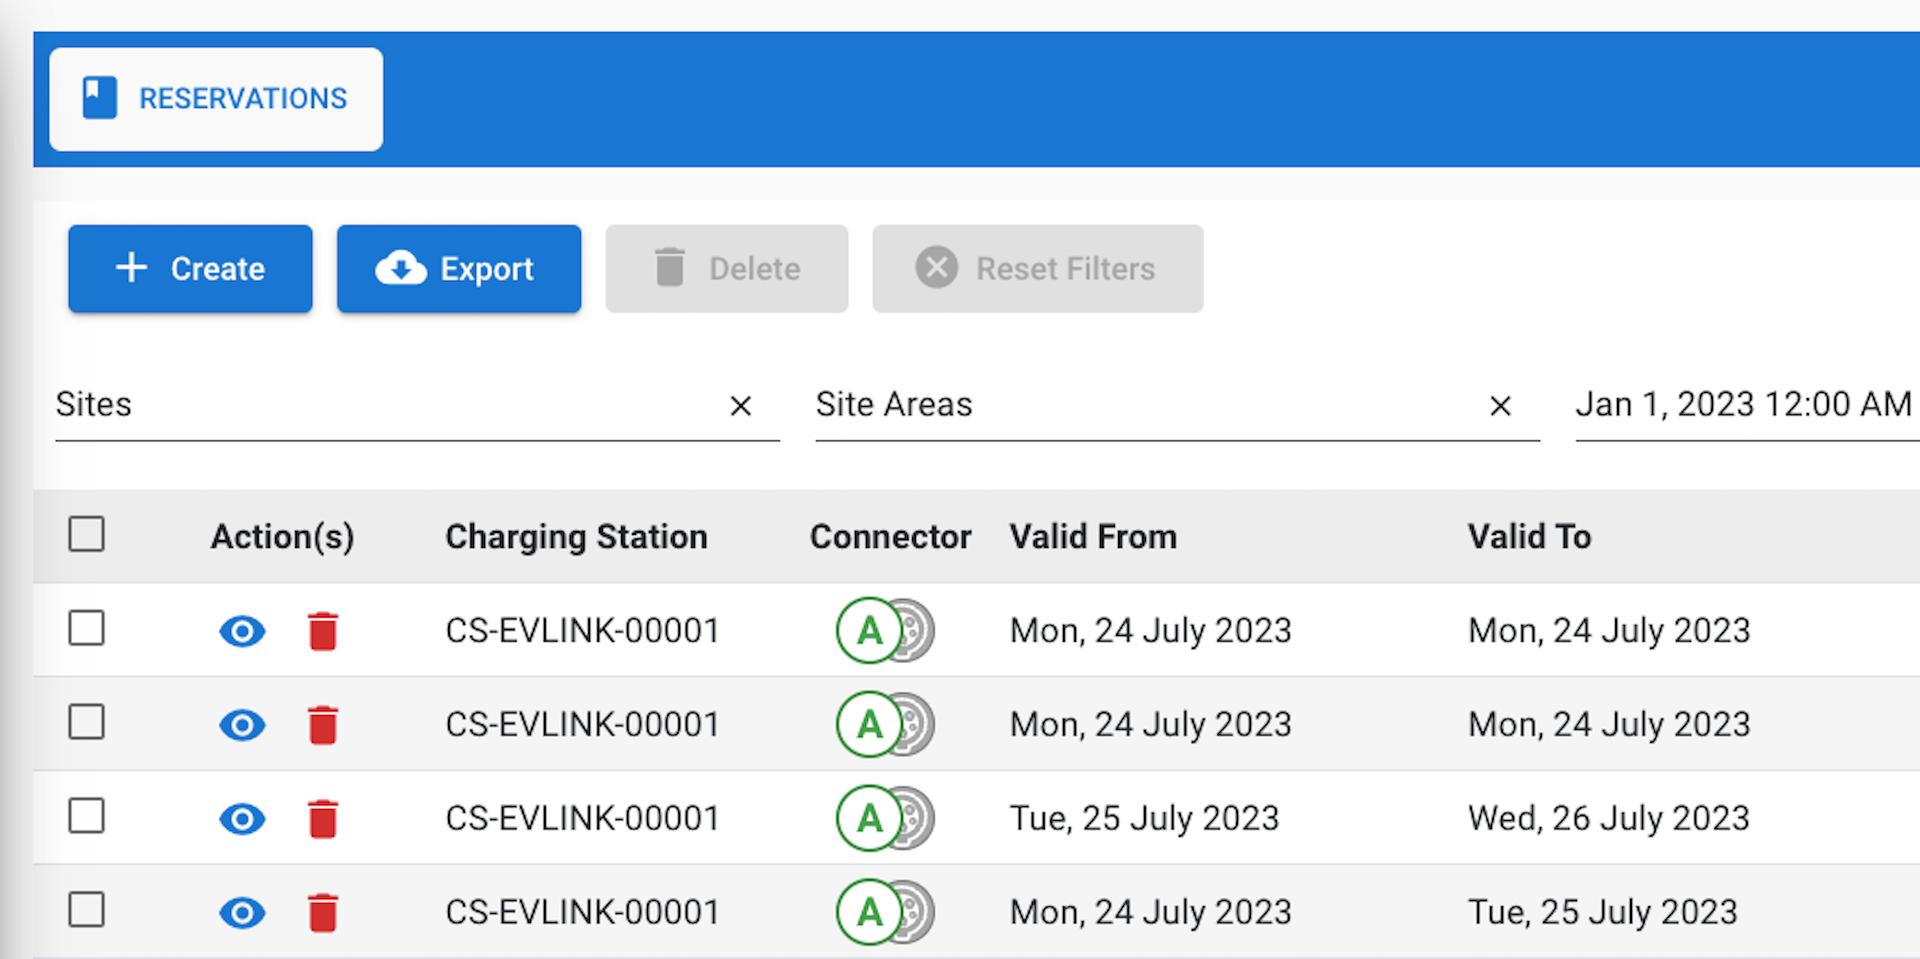
\includegraphics[width=\textwidth]{resources/images/main/6_implementation/screens/delete_reservation/web/Delete_Reservation.png}
         \captionsetup{skip=58pt}
         \caption{Delete a reservation in the browser.}
         \label{fig:web-delete-reservation-impl}
    \end{subfigure}
     \hfill
     \begin{subfigure}[c]{0.3\textwidth}
        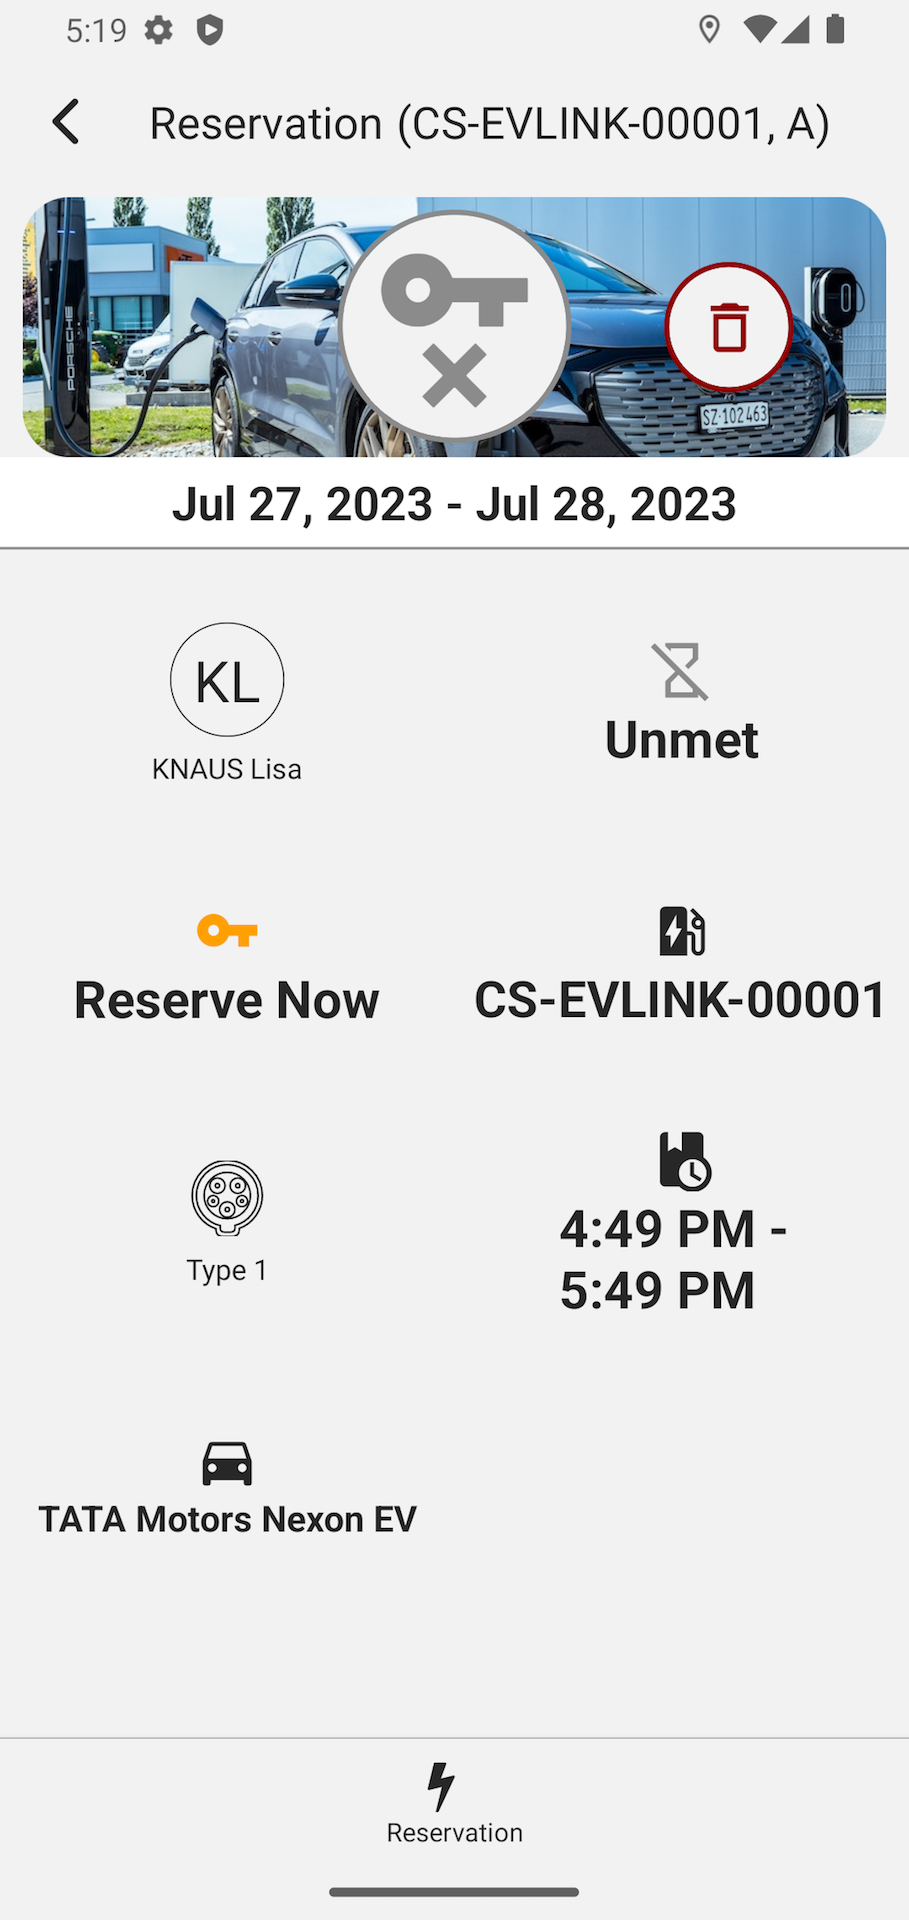
\includegraphics[width=\textwidth,height=1.5\textwidth,keepaspectratio]{resources/images/main/6_implementation/screens/delete_reservation/mobile/Delete_Reservation.png}
         \caption{Delete a reservation on the hand--held device.}
         \label{fig:mobile-delete-reservation-impl}
    \end{subfigure}
    \caption{Implementation of the user interfaces of the mobile and web application relating to the deletion of reservations using the \faIcon[solid]{trash} icon.}
    \label{fig:impl-delete-reservation}
\end{figure}

\noindent To allow both atomic and batch deletion of entities, the \acrshort{rest} methodology recommends introducing the endpoints listed in Table \ref{tab:delete-reservation-rest}. 
For distinguishing between both operations, in order to delete a single object, the user must reference it by its \acrshort{id}. 
In the case of deleting multiple entries, the user has to submit multiple entries, omitting the \acrshort{id} path parameter.

\begingroup
\setlength{\tabcolsep}{10pt} % Default value: 6pt
\renewcommand{\arraystretch}{1.5} % Default value: 1
\begin{table}[h]
\centering
\caption{\acrshort{rest} endpoints for deletion purposes.}
    \begin{tabular}{l|c}
    Resource Identifier & HTTP Method \\ \hline
    \texttt{/reservations/} & \texttt{DELETE} \\
    \texttt{/reservations/\{id\}/} & \texttt{DELETE}
    \end{tabular}
\label{tab:delete-reservation-rest}
\end{table}
\endgroup

\newpage

\subsubsection{Enable Reservations}
\label{ch:Implementation:sec:Reservation System:ssec:Management Capabilities:sssec:Enable Reservations}

Representing the final predefined management capability established during the preceding design phase, the \textbf{Enable Reservations} function enables the system administrator to activate the extension developed in this work.
This feature is part of the \texttt{Tenant Component} modules, which stand for different feature sets, the tenants can be enabled for.  
Due to the varying requirements and challenges faced by each organization, as identified by their dedicated tenant, the range of usable functionalities differs significantly. Which only requires subsets of the system's feature sets to be enabled simultaneously.
However, certain dependencies exist between the various components, which necessitate activating specific ones, in order to enable the usability as a whole. The reason for this is that each module determines the amount of data and information available to the tenant, therefore, activating a certain group of components is logical.
For example, the tenant component \texttt{Reservation} depends on the corresponding \texttt{Organization} component to get access to the \acrshortpl{cs} on the different sites of the organization and the relevant users. Otherwise, the system denies to enable this component on itself.
Components such as the \texttt{Car} component may be activated upon request, to offer a wider range of features to the particular component. In the case of the \texttt{Reservation} component, this enables the integration of cars into the reservation.
The example configuration within the administration area of the web frontend for enabling components is displayed in the following Figure \ref{fig:enable-reservation-impl}.

\begin{figure}[h]
    \centering
    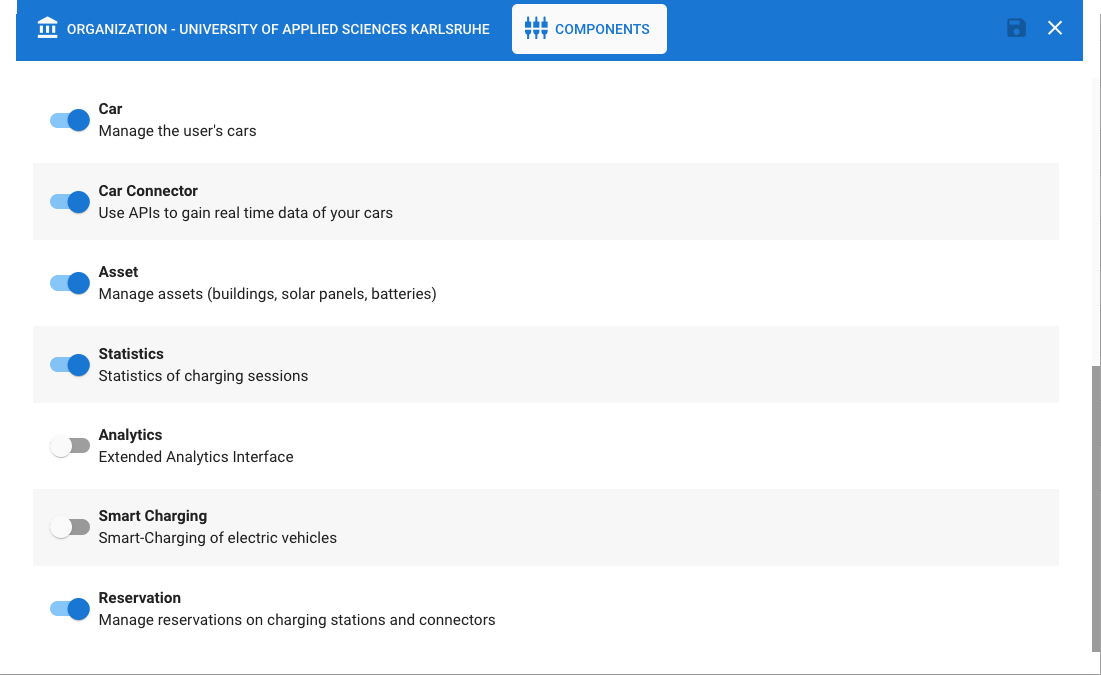
\includegraphics[width=0.8\textwidth,keepaspectratio]{resources/images/main/6_implementation/screens/enable_reservations/Reservation_Module.png}
    \caption{Implementation of the user interface for enabling the reservation module.}
    \label{fig:enable-reservation-impl}
\end{figure}

\noindent If the \texttt{Reservation} component is not active, the adjusted solution provides solely the basic \acrshort{ocpp} reservation feature set, using the standard \textit{ReserveNow} and \textit{Cancel Reservation} operations \cite{noauthor_ocpp_nodate}. 
This does not include the extension of recurring and reservations in advance, as discussed in Section \ref{ch:Implementation:sec:System Prerequisites}.

\subsection{Scheduling Capabilities}
\label{ch:Implementation:sec:Reservation System:ssec:Scheduling Capabilities}

Complementing the management capabilities covered in the previous subsection \ref{ch:Implementation:sec:Reservation System:ssec:Management Capabilities}, the ability to schedule and process pre--configured tasks automatically without any interaction is a key aspect of developing a system that manages distributed infrastructure facilities. 
To maximize automation, the proposed scheduling capabilities comprise a set of batch processing jobs, that are intended to run sequentially and can be enabled on demand within the \acrshort{json} configuration file \texttt{src/assets/config.json} included with the project. 
In addition to task activation and ensuring the specified sequential order, this file also allows for specifying the execution intervals in the form of \texttt{*/1 * * * *}, employed as the syntax for Cron jobs in the \textit{UNIX} world, to schedule job processing at specific times.
For the execution to behave as expected, the reservation component module introduced in \ref{ch:Implementation:sec:Reservation System:ssec:Management Capabilities:sssec:Enable Reservations} must be enabled. Otherwise, regardless of the activation, these tasks are not running.
The pivotal function for handling these tasks is represented by the \texttt{TenantSchedulerTask} already mentioned as one of the key components for the working system in \ref{ch:Implementation:sec:Reservation System:ssec:Architectural Views:sssec:Components}.
As the top--level entity overseeing all available tasks for execution, it executes the activated ones at their designated time intervals on the server.
The recommended sequence for executing the subsequent jobs to ensure correct operation is defined as follows within the context of this work:
\begin{description}
    \item[]{\makebox[5.5cm][l]{\textbf{Schedule Reservation:}} \texttt{*/5 * * * *} \quad \textit{'Executed every five minutes.'}}
    \item[]{\makebox[5.5cm][l]{\textbf{Expire Reservation:}} \texttt{*/4 * * * *} \quad \textit{'Executed every four minutes.'}}
    \item[]{\makebox[5.5cm][l]{\textbf{Free Reserved Connectors:}} \texttt{*/1 * * * *} \quad \textit{'Executed on a minute basis.'}}
\end{description}

\newpage

\subsubsection{Schedule Reservation}
\label{ch:Implementation:sec:Reservation System:ssec:Scheduling Capabilities:sssec:Schedule Reservation}

Due to the fact that the user can create reservations in the future, the corresponding \acrshortpl{cs} and the system itself must be notified when the reserved time period arrives. \\
To do this, the \textbf{Schedule Reservation} task shown in Figure \ref{fig:schedule-reservation-seqflow}, implemented as \\ \texttt{SynchronizeReservationTask}, loads all reservations with status \texttt{SCHEDULED} for the next 15 minutes from the database.
Also, to enable recurrent events, this comprises bookings with the status \texttt{IN\_PROGRESS} as well. 
In the further processing of the combined booking types, the \texttt{synchronizeWithChargingStation} method checks for currently running charging sessions on the respective stations and connectors. If these sessions are not assigned to the \acrshort{rfid} tag, that belongs to the reservation, the method stops them immediately.
To address this, the \texttt{ChargingStationClient} is used, which is a product of the \texttt{ChargingStationClientFactory}, that controls instantiation using factory methods, to communicate directly with the \acrshort{cs}.
Otherwise, the reservation is made directly on the \acrshort{cs} and if it has a \texttt{SCHEDULED} status, it is adjusted accordingly. A notification is then sent to the user, via the \texttt{NotificationHelper}, to inform that a booked charging session is forthcoming.
Besides saving the updated record, its \acrshort{id} is assigned to the associating connector on the \acrshort{cs} in the database, using the \texttt{updateConnectorWithReservation} method.

\begin{figure}[h]
    \centering
    \includegraphics[width=0.8\textwidth,keepaspectratio]{resources/images/main/6_implementation/processes/scheduler/SynchronizeReservation.png}
    \caption{Interaction between relevant components to synchronize the reservations with the associated \acrshortpl{cs} taking into account the underlying process design.}
    \label{fig:schedule-reservation-seqflow}
\end{figure}

\newpage

\subsubsection{Expire Reservation}
\label{ch:Implementation:sec:Reservation System:ssec:Scheduling Capabilities:sssec:Expire Reservation}

After having automatically synchronized the reservations with the corresponding \acrshortpl{cs}, a routine to clean up the expired ones and to fulfill certain aspects of the householding tasks is implemented as \texttt{CheckReservationStatusTask}.
Designed as a counter piece to \textbf{Schedule Reservation}, this job deals with entities reaching their expiration date, as demonstrated in Figure \ref{fig:expire-reservation-seqflow}.
To identify the concerned bookings, it loads each record with a status of \texttt{IN\_PROGRESS} or \texttt{SCHEDULED} and an expiry date that is overdue by the current time and date.
If any record is found, the task then iterates through the list of reservations and removes the reservation information from the associated connector, using \texttt{resetConnectorReservation}. 
As a complement to the \texttt{updateConnectorWithReservation} function mentioned in the previous process, this method is used when an arrangement still blocks a connector after it is successfully cancelled or deletion. This is often due to the system disconnecting from the \acrshort{cs} during the latter stages of the process.
Considering this case, it is utilized to invalidate expired bookings, change their status to \texttt{EXPIRED} in the database, and notify the involved profile with the \texttt{NotificationHelper}.

\begin{figure}[h]
    \centering
    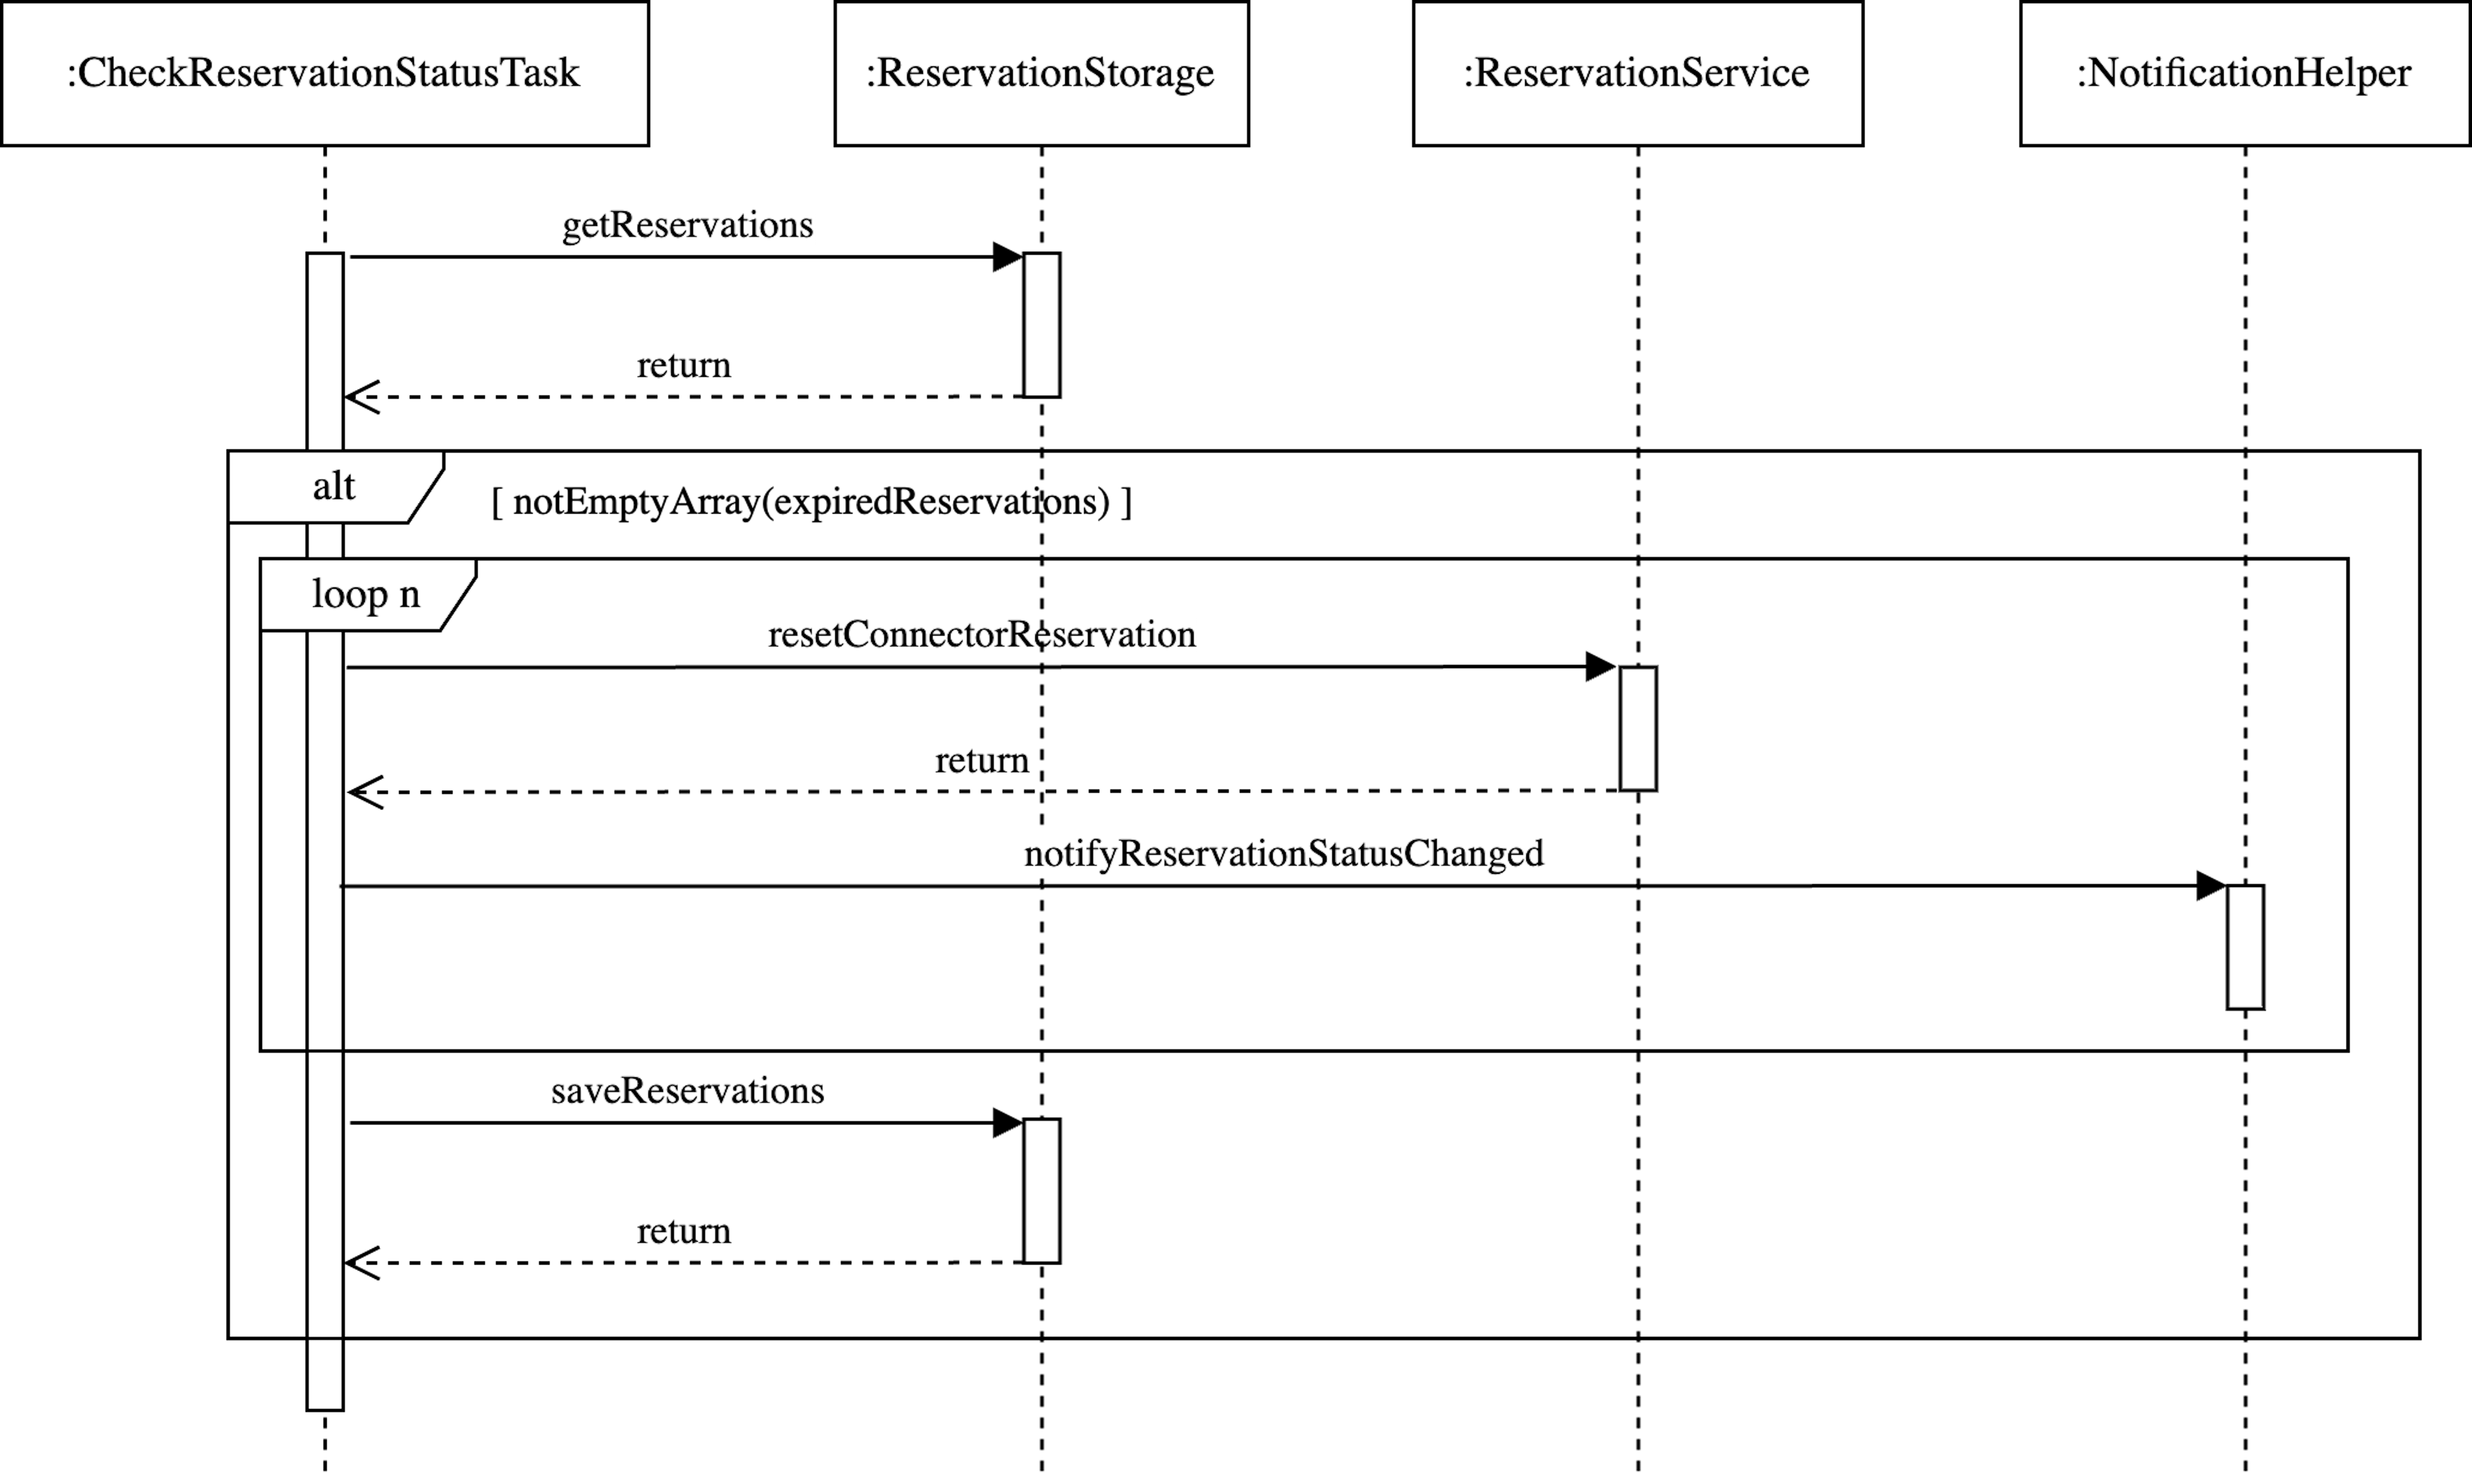
\includegraphics[width=0.8\textwidth,keepaspectratio]{resources/images/main/6_implementation/processes/scheduler/UpdateExpiredReservations.png}
    \caption{Sequential flow of the components interacting with each other, to invalidate expired bookings using the considered process templates.}
    \label{fig:expire-reservation-seqflow}
\end{figure}

\newpage

\subsubsection{Free Reserved Connectors}
\label{ch:Implementation:sec:Reservation System:ssec:Scheduling Capabilities:sssec:Free Reserved Connectors}

While the \textbf{Expire Reservation} function looks after the expiry as a natural element of the booking life cycle, the \textbf{Free Reserved Connectors} task has a more regulative purpose.
Taking the position of an imaginary steward, it monitors all ongoing engagements on the \acrshortpl{cs} and identifies the ones, where the user has not arrived after a certain period of time after the supposed arrival time.
Following the \acrshort{ocpp} standard, the arrangement lasts until the expiry time is reached. As the expiration time is undefined, it could be several hours later and block the station during this time. 
To mitigate this issue in the handling of reservations, the proposal provides a background task, implemented in \texttt{CancelUnmetReservationsTask} and described in Figure \ref{fig:free-connector-seqflow}.
As a result of this custom implementation, it is possible to handle unfulfilled reservations, due to a certain threshold defined by the constant \texttt{THRESHOLD}, which is set to \textbf{15} minutes in the context of this work.
Every booking with an arrival time exceeding this threshold is identified by the \texttt{ReservationStorage}. If the associated connector is still in the \texttt{RESERVED} state, the blockage is cancelled to free the reserved charging unit.
Otherwise, the next one is evaluated by using these constraints.
After setting all identified entries meeting these criteria to the \texttt{UNMET} status and saving them again, the relevant individuals are informed of their undesired conduct.

\begin{figure}[h]
    \centering
    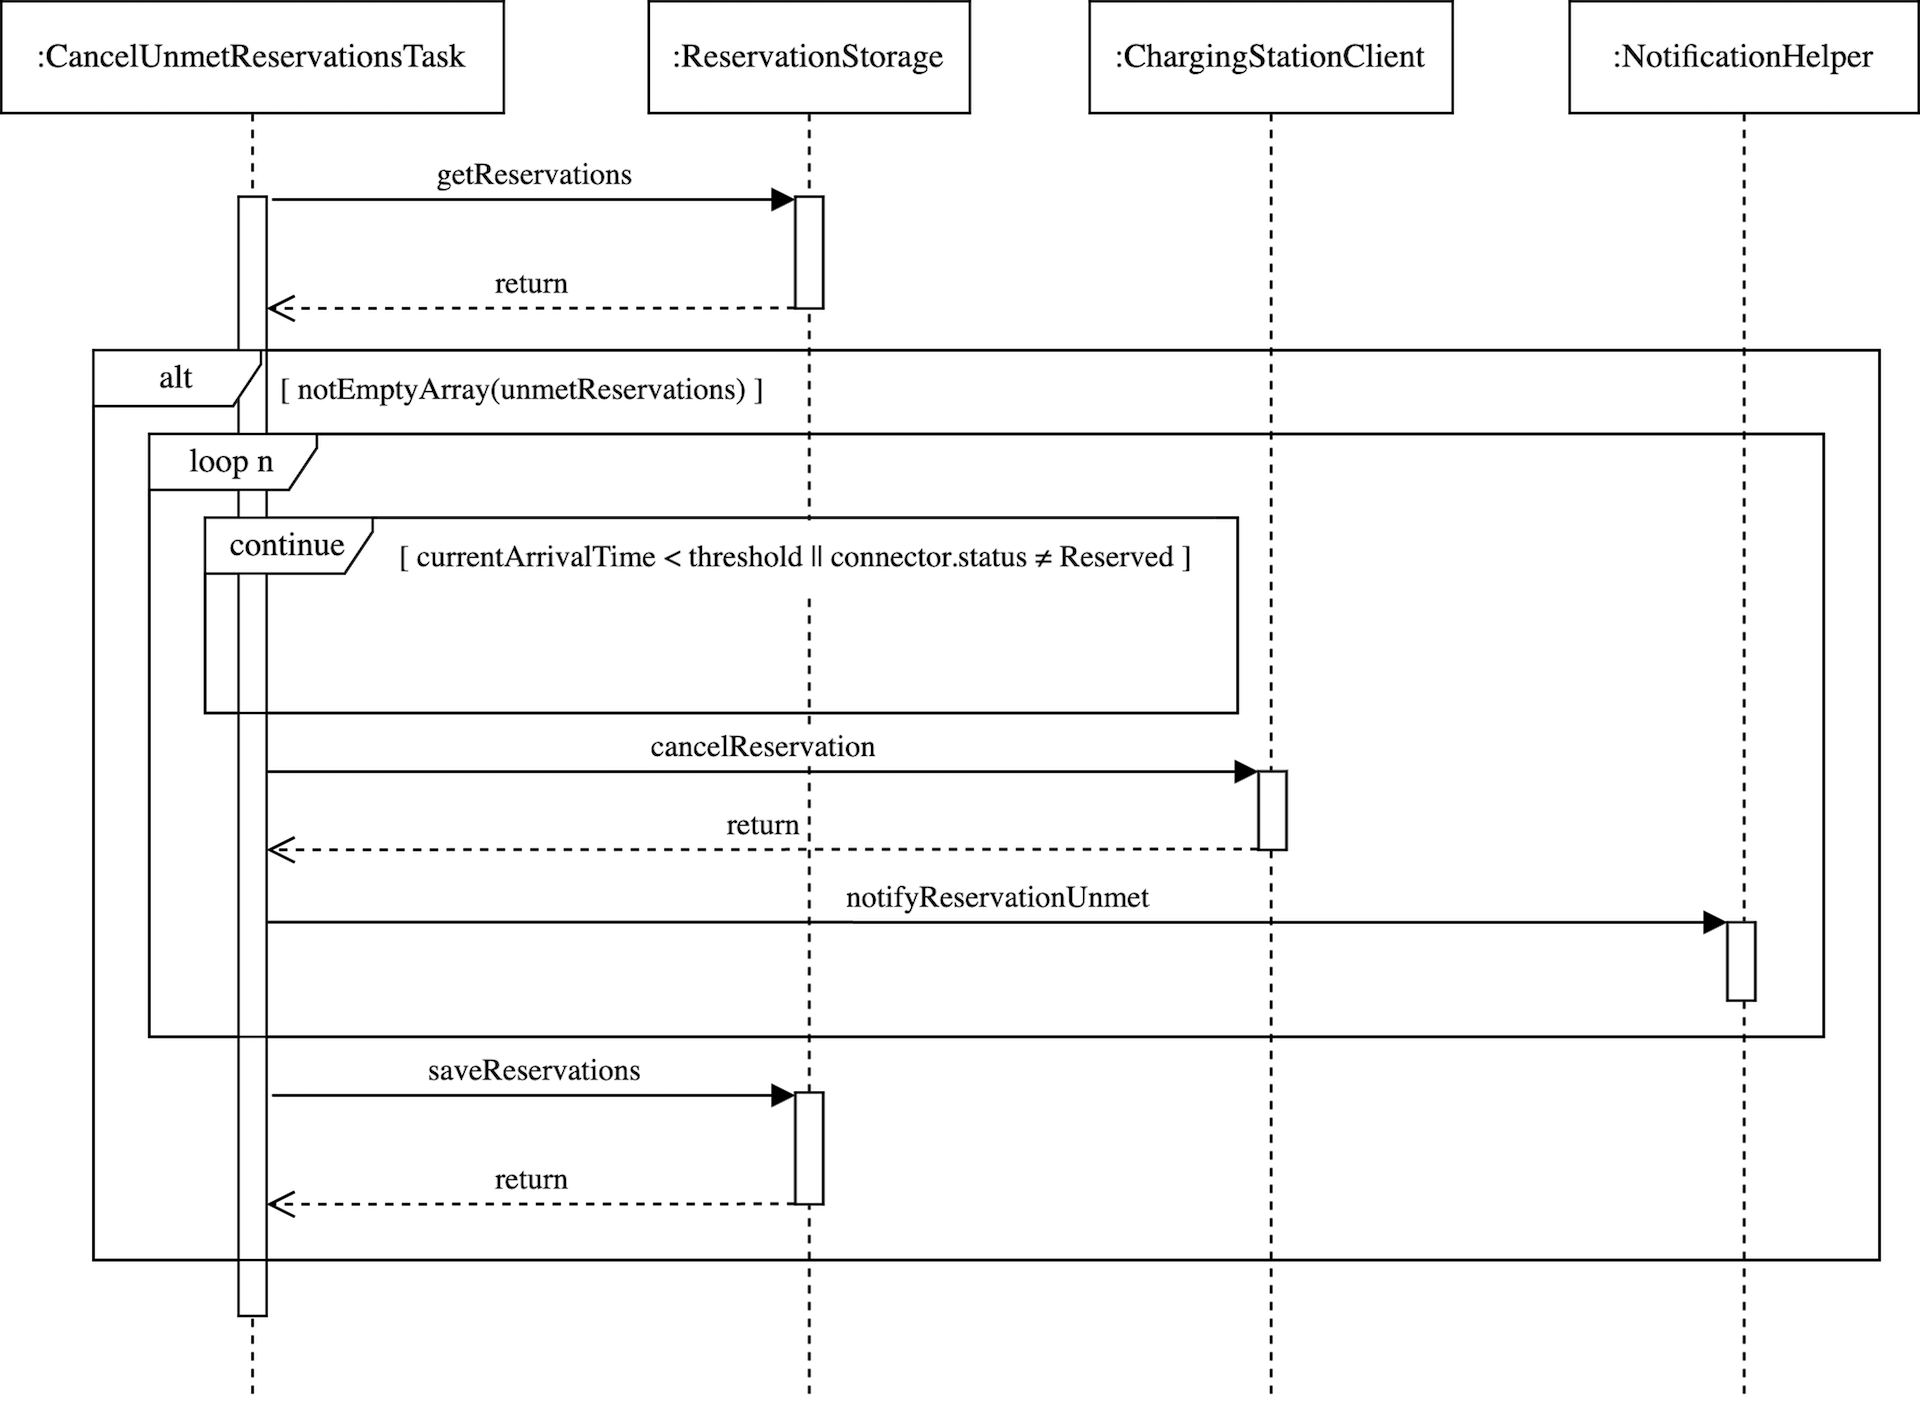
\includegraphics[width=0.8\textwidth,keepaspectratio]{resources/images/main/6_implementation/processes/scheduler/CancelUnmetReservation.png}
    \caption{Required component interactions for removing unmet appointments on the respective \acrshortpl{cs} in order to implement the underlying design proposals.}
    \label{fig:free-connector-seqflow}
\end{figure}

\newpage

\subsection{Notification Capabilities}
\label{ch:Implementation:sec:Reservation System:ssec:Notification Capabilities}

With regard to the notification types, introduced to cover different scenarios in the application and arrangement lifetime, this subsection provides a brief overview of which notification types are actually used within the implemented features.
This may serve as a reference point for future implementations and as a possibility to evaluate new scenarios not covered by this implementation.
Implied by the listing of involved packages in subsubsection \ref{ch:Implementation:sec:Reservation System:ssec:Architectural Views:sssec:Packages}, particularly by viewing the \texttt{notification} package, the system can send notifications in various forms.
Alongside using the \acrshort{smtp} protocol \cite{klensin_simple_2008} primarily targeting adopters of the browser app with assumed easier access to their mail clients, for the mobile apps the service utilizes Google's Firebase \cite{noauthor_firebase_nodate} \acrshort{paas} and \acrshort{iaas} offer to publish information via push notifications.
During the development phase as part of the extension for the mobile component of the project, this work has identified missing functionalities related to background notifications, when the application is closed or not opened. To address this specific feature gap, adjustments to the appropriate logic and the \texttt{notifee/react-native} package from Notifee \cite{noauthor_notifee_nodate} are added.
Seizing the suggestions represented by \textbf{Scheduling Capabilities} in Subsection \ref{ch:Design:sec:Reservation System:ssec:Scheduling Capabilities} of the design chapter, the notification types such as \texttt{ReservationStatusChanged}, \texttt{ReservationUpcoming}, \texttt{ReservationCreated}, \texttt{ReservationCancelled} and \texttt{ReservationUnmet} are utilized in the current tasks to convey crucial information about the processed entities to the end users and facilitate the information flow.
This should ensure that the \acrshort{evu} can make informed decisions based on up--to--date information provided by the system.
In the case of the \texttt{ChargingStationBlocked} notification, no suitable location could be identified. An integration within the \textbf{Schedule Reservation} process would lead to a simultaneous notification of the user blocking the \acrshort{cs}, as well as the user of the reservation. 
Possibly resulting in the parallel switching of drivers to a new station and the situation that this notification was intended to prevent. \\
\noindent In terms of the support for multiple languages both the notifications and the labels of the \acrshort{gui} elements, which normally adapt to the language set in the user's profile, are only translated into English and German.
Other language options, including Spanish, French, and Italian, are not part of this approach and further work needs to be done to allow these languages to be used properly.

\newpage

\subsection{Additional Capabilities}
\label{ch:Implementation:sec:Reservation System:ssec:Additional Capabilities}

During development, more ways to enhance the reservation approach with extended features beyond the defined use cases could be identified.
These capabilities, since they have no direct use affecting the basic functionality in interaction with the system, are listed as \textbf{Additional Capabilities} and are mentioned here as part of an informative section, to possibly be considered as useful for other scenarios, that may arise during other studies in this area.

\subsubsection{Export Reservation}
\label{ch:Implementation:sec:Reservation System:ssec:Additional Capabilities:sssec:Export Reservation}

By examining the backend service features and frontends' specific functions, the potential to export certain entities of the system in the form of generated \acrshort{csv} reports stands out.
Despite the fact that it was not considered during the design of the system, the author of the work assumes that this feature could be useful for the end users of the platform in the context of data recovery and analysis purposes.
Representing a very basic functionality, which only requires extracting all specified entries from the database and transforming them into a \acrshort{csv} compliant format, no additional process or sequence flow is elaborated.
Implemented as a button on the reservation overview interface within the web \acrshort{gui}, the \textbf{Export Reservation} functionality loads each booking the user has access to from the database and writes the entries into a \acrshort{csv} compliant file that can be downloaded via the browser.
If the database crashes or there is a risk of unwanted data loss, these files could be the basis for populating new instances of the system or recreating a clean application state.

\noindent As a dedicated endpoint on the web server, this functionality is provided, using the \acrshort{rest} methodology and the relevant resources as part of the service portfolio and is presented in the subsequent Table \ref{tab:export-reservation-rest}.

\begingroup
\setlength{\tabcolsep}{10pt} % Default value: 6pt
\renewcommand{\arraystretch}{1.5} % Default value: 1
\begin{table}[h]
\centering
\caption{Endpoint for exporting the booking entries inside the database.}
    \begin{tabular}{l|c}
    Resource Identifier & HTTP Method \\ \hline
    \texttt{/reservations/action/export} & \texttt{GET}
    \end{tabular}
\label{tab:export-reservation-rest}
\end{table}
\endgroup

\subsubsection{Reservable Charging Stations}
\label{ch:Implementation:sec:Reservation System:ssec:Additional Capabilities:sssec:Reservable Charging Stations}

Due to the assumption, that the individuals create their reservations directly by selecting the \acrshortpl{cs} from the map view, considered as the entry point of the mobile application, or by using the various filter options within the web app, a pre--filtering mechanism to narrow down the options for available stations during a specific time in the future was not included in the design.
However, the proposed solution provides a method for making bookings without pre--selecting the \acrshort{cs}, which leads to the requirement of choosing a suitable station, while setting the reservation constraints. To promote a more convenient recommendation mechanism, the creation process should be supported by minimizing the number of stations presented, that are not otherwise occupied at the given time.
Taking this into account, the initial concept of the underlying logic resembles a simple intersection, similar to the one shown in Figure \ref{fig:reservable-cs}. In this way, the appropriate subset of connectors available for reservation could be easily identified.
Hence, the code loads all the entries for the specified period and all the \acrshortpl{evse} registered in the system, in order to perform an intersection of the two sets and select only the stations inside the \textbf{blue area}, as shown in the diagram below. These stations comprise the subset of options to be offered by the input fields.
If other \acrshortpl{evu} create reservations during this process, that would affect the offered selection, the service should detect any resulting overlaps and handle them appropriately as usual.

\begin{figure}[h]
    \centering
    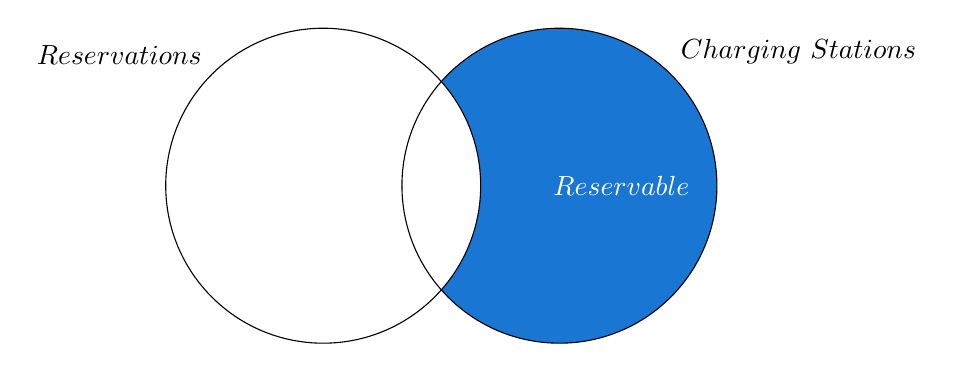
\begin{tikzpicture}[
        set/.style = { circle, minimum size=4cm}]
        \node[set,fill=blueprimary,label={45:$Charging\ Stations$}] (cs) at (0:3) {};
        \node[set,fill=white,label={135:$Reservations$}] (r) at (0,0) {};
        \draw (0,0) circle(2.0cm);
        \draw (3,0) circle(2.0cm);
        \node[right,white,xshift=-0.2cm] at (cs.center){$Reservable$};
    \end{tikzpicture}
    \caption{Isolation of reservable \acrshortpl{cs} utilizing an intersection with already reserved ones.}
    \label{fig:reservable-cs}
\end{figure}

\noindent As the client applications must pre--populate input fields in the appropriate \acrshort{gui} windows, this supporting functionality is triggered by the respective endpoints listed in the Table \ref{tab:reservable-cs-rest}. To implement this feature, the selected design approach requires expanding the relevant \texttt{charging-station} \acrshort{rest} resource, which is managed by the \texttt{ChargingStationService} and the upstream \texttt{ChargingStationRouter}.

\begingroup
\setlength{\tabcolsep}{10pt} % Default value: 6pt
\renewcommand{\arraystretch}{1.5} % Default value: 1
\begin{table}[h]
\centering
\caption{Added \acrshort{rest} endpoint to provide the subset of reservable \acrshortpl{cs}.}
    \begin{tabular}{l|c}
    Resource Identifier & HTTP Method \\ \hline
    \texttt{/charging-stations/reservation/availability} & \texttt{GET}
    \end{tabular}
\label{tab:reservable-cs-rest}
\end{table}
\endgroup

\newpage

\subsubsection{Reservation Retrieval}
\label{ch:Implementation:sec:Reservation System:ssec:Additional Capabilities:sssec:Reservation Retrieval}

Besides the aforementioned feature sets and their related endpoints, a web service following the \acrshort{rest} architectural model requires additional interfaces, e.g. for information retrieval.
Consequently, according to this approach, endpoints must be supplied for so--called \texttt{READ} operations. The function's connotation implies, that these endpoints are accessible for requesting data when calling the corresponding \acrshort{url}.
Following the naming convention of the \acrshort{rest} method, the resource for collecting reservations is declared, as its plural form of the handled entity name in lowercase. Given the proposed solution and the reservation as the underlying entity, the resource provided by this system is called \texttt{reservations}.
Resulting in the interfaces listed in Table \ref{tab:read-reservations-rest} and accessible through the reservation \acrshort{api}, mainly employed for providing clients access to the internal system information.

\begingroup
\setlength{\tabcolsep}{10pt} % Default value: 6pt
\renewcommand{\arraystretch}{1.5} % Default value: 1
\begin{table}[h]
\centering
\caption{\acrshort{rest} endpoints for performing \texttt{READ} operations retrieving reservation entities.}
    \begin{tabular}{l|c|m{5cm}}
    Resource Identifier & HTTP Method & Functionality \\ \hline
    \multicolumn{3}{c}{\texttt{/reservations}} \\ \hline
    \texttt{/} & \texttt{GET} & Retrieve all reservations available \\
    \texttt{/\{id\}} & \texttt{GET} & Request for a specific reservation by its \acrshort{id} \\
    \end{tabular}
\label{tab:read-reservations-rest}
\end{table}
\endgroup

\subsection{Role Concept}
\label{ch:Implementation:sec:Reservation System:ssec:Role Concept}

To assign the necessary functionality to each system role, as described in the chapter of requirements engineering, particularly Section \ref{ch:Requirements Engineering:sec:Role Mapping}, the capabilities required to fulfill their purpose must be considered according to the principles of least privilege, which are explained in \cite{ma_specifying_2011}.
Additionally, to supplement the mapping of feature sets to roles, the solution distinguishes between specific scopes that describe the range of information available to that particular role.
Roles assigned with the \textit{Own} scope only have access to their own data and cannot view reservations made by other profiles, for example.
That falls within the scope of the \textit{Site}, allowing the assigned role to access all data pertaining to that specific location.
With this privilege, the respective user can create, update, or cancel bookings for all users assigned to this site, for instance. An exception to this privilege set is the \textit{Admin} role, which is not limited to a dedicated site and allows the user to manage all entities, related to the entire tenant. 
Concerning the use cases from Chapter \ref{ch:Requirements Engineering} and their associated actors, the final mapping of the developed processes is presented in Table \ref{tab:role-function-mapping} as defined in the file \texttt{AuthorizationsDefinition.ts} as part of the backend project.

\begingroup
\setlength{\tabcolsep}{10pt} % Default value: 6pt
\renewcommand{\arraystretch}{1.5} % Default value: 1
\begin{table}[h]
    \centering
    \caption{Mapping of the designated reservation functionalities to the corresponding roles in the system.}
    \begin{tabular}{c|c|m{9.5cm}}
        Role & Scope & Functionality \\
        \hline
        Basic & Own & Create Reservation, Update Reservation, Cancel Reservation \\
        Admin & - & Create Reservation, Update Reservation, Cancel Reservation, Delete Reservation \\
        Site Admin & Site & Create Reservation, Update Reservation, Cancel Reservation \\
        Site Owner & Site & Create Reservation, Update Reservation, Cancel Reservation \\
        Super Admin & - & Enable Reservations \\
        Demo & Own & Create Reservation, Update Reservation, Cancel Reservation \\
    \end{tabular}
    \label{tab:role-function-mapping}
\end{table}
\endgroup

\newpage

\noindent Afterwards, the assignment decisions in the context of the \textit{Delete Reservation} and \textit{Enable Reservations} actions are revisited, for a better understanding. The choice to only allow the \textit{Admin} user to perform the \textit{Delete Reservation} action is not solely based on the use case design.
This work assumes, that disruptive actions, such as entity deletion, should only be carried out when excluding system users and removing their information, which can be classified as an administrative task and solely limited to system administrators.
Concerning basic users, it is more likely that they use the cancel operation to properly revoke their reservations than to delete them completely.
In the case of the \textit{Enable Reservations} task, only the \textit{Super Admin} can access the relevant sections of the administration dashboard to configure the tenants, thus, making this role the exclusive entity for assigning this feature. 
On the other hand, this profile is unable to manage entities within the particular tenants itself, hence the need to assign it additional privileges for managing reservations is mandatory. 

\newpage

\subsection{Failure Indication}
\label{ch:Implementation:sec:Reservation System:ssec:Failure Indication}

The introduction of new features not only creates new possibilities for the interaction with the audience but also opens up a wider surface for possible unexpected circumstances, that may arise along certain scenarios. 
Most of these exceptions may occur in a way that only the system can recognize and are typically hidden from the user, who is simply experiencing the consequences, resulting from these malfunctions.
To alleviate these uncertainties, a software solution should always inform the user of its current status within the process it performs. This involves notifying the client, on behalf of the user, of any unexpected behavior that could interrupt the current operation or lead to a bad result.
Due to the nature of distributed systems, the client and the corresponding server are decoupled, and the only way the server could keep the client informed of the above scenarios is to use the \acrshort{http} status codes as part of each request to exchange information.
Apart from failures within the system itself in the form of outages or targeted attacks, the charging infrastructure and the associated \acrshortpl{cs}, should also be considered as an extra source of errors. 
To effectively identify and manage exceptions in both the backend and frontend applications, this study translated each potential exception into a status code for meaningful reservation error handling.

\noindent The list below only reflects the current state of implementation, concerning the aforementioned range of capabilities, as well as the current state of the \acrshort{ocpp} standard, which is not meant to be complete. Potentially, additional scenarios and relevant exception--handling mechanisms need to be incorporated in the future.

\begin{multicols}{2}
\begin{description}
    \item[\texttt{600}] Reservation Already Exists
    \item[\texttt{601}] Reservation Collision
    \item[\texttt{602}] Reservation Not Supported *
    \item[\texttt{603}] Reservation Rejected *
    \item[\texttt{604}] Reservation Faulted *
\end{description}
\begin{description}
    \item[\texttt{605}] Reservation Occupied *
    \item[\texttt{606}] Reservation Unavailable *
    \item[\texttt{607}] Multiple Reserve Now
    \item[\texttt{608}] Invalid Status Transition Error
\end{description}
\end{multicols}

\noindent To distinguish the exceptions that may arise from the charging infrastructure, the respective entries in the above list are marked with the * symbol. For a detailed explanation of these particular error scenarios, please refer to the official \acrshort{ocpp} standard \cite{noauthor_ocpp_nodate}.

%% LaTeX2e class for student theses
%% sections/main/7_validation.tex
%%
%% Karlsruhe University of Applied Sciences
%% Faculty of Computer Science and Business Information Systems
%%
%% --------------------------------------------------------
%% | Derived from sdqthesis by Erik Burger burger@kit.edu |
%% --------------------------------------------------------

\chapter{Analysis and Validation}
\label{ch:Analysis and Validation}

Referring to the final design concept and its implementation within the practical part of this work, the proposed reservation system and its capabilities, which are considered necessary for an efficient management of the charging infrastructure, are observed in an evaluative manner and finally reviewed.
Therefore, the assumptions formulated during conceptualization, as well as the pre-defined goals and their achievement, are considered to give a reasonable assumption of whether the system is capable of handling reservations on \acrshortpl{cs} in an efficient manner.
Alongside the stated objectives for fulfilment, this chapter discusses open issues that emerged during the different phases and which could not be integrated into the development process due to the limited resources available. However, these characteristics are deemed essential to facilitate situations that would add value to this work.
To conclude the capabilities listed and further possibilities for feature implementations, the limitations of such a system, described in the final part of this chapter, are elaborated as a set of challenges in the context of certain scenarios. 

\section{Achievement of Objectives}
\label{ch:Analysis and Validation:sec:Achievement of Objectives}

With the aim of elaborating a reservation process implemented insight a suitable system for handling the relevant charging infrastructure, this thesis stated several objectives that the system needs to satisfy. 
Formulated in the \textbf{Goals} section \ref{ch:Requirements Engineering:sec:Goals} within the preliminary \textbf{Design} chapter, the fulfilment of these goals is subsequently evaluated.
Beginning with a brief summary of each goal, the capabilities addressed are evaluated in relation to their originally proposed range of functionality.
%% --------------------------------------------------------
%% Goal 1 - Management Capabilities
%% --------------------------------------------------------
Regarding the regulation and management of entities within a software solution, it requires specific basic operations to carry out the tasks, mainly known as '\textbf{Management Capabilities}'.
As stated in the first objective, a reservation system's crucial feature is the ability to manage various types of reservations. This includes criteria to prevent overlaps and collisions, along with the flexibility to modify, reschedule, or cancel individual appointments.
Since not every user in the system has the same privileges based on the role assigned to their profile, rules governing access to the range of functionality provided, as well as the associated insight into the data available, are part of this consideration and should be enforced by the system.
%% --------------------------------------------------------
%% Goal 2 - Self-Healing and Autonomous Processes
%% --------------------------------------------------------
With access control rules in mind, the concept of '\textbf{Self-Healing and Autonomous Processes}' arising from a set of rules covering the description of a self-regulated behavior that allows the system to handle pre-conceived scenarios without the intervention of a user, is defined as the second objective. 
In addition to mitigating undesired actions of individuals, the transition of managed entities, such as changing their states according to specific constraints, is conceivable.
Consequently, both the convenience of the system user, who no longer needs to approve and process each step of the entity life cycle, and the consistency of the data could be improved.
%% --------------------------------------------------------
%% Goal 3 - Support of relevant standards
%% --------------------------------------------------------
Beyond the capabilities, which focus on the systems' functionalities and the support of generic functions to enable the user to achieve his goals, the environment and the communication partners that exchange data with the solution need to be also addressed.
Due to the emphasis on the charging infrastructure in the context of \acrshort{emobility} and the recharging of \acrshortpl{ev}, the industry and other players in the field have developed a common basis as a guideline for communication between the various entities involved in the domain.
Representing these guiding principles, which include the definition of a basic feature set in combination with the essential steps to achieve successful interaction with the relevant devices, standards such as those mentioned in \ref{ch:Fundamentals:sec:Electric Mobility:ssec:Relevant Standards} need to be considered.
Covered by the '\textbf{Support of relevant standards}', the intention is to provide an interoperable solution that is not restricted to a particular type of infrastructure but can manage all devices that implement the generally accepted standards.
%% --------------------------------------------------------
%% Goal 4 - Modular Design
%% --------------------------------------------------------
After gathering the required functionalities and referencing the relevant standards that the system must consider, the objective of '\textbf{Module Design}' focuses on addressing the design of the solution in terms of software components and the necessary abstraction from the remaining system landscape.
Resulting in the ambition to provide as much decoupling as possible, which promotes both resiliency of the overall system in case of failure, and easier carve-out of functionality for individual service deployments. Furthermore, this permits integration within other services or the potential for reuse within other deployment scenarios. \\

\noindent Considering the above objectives and their relation to the current output, the following conclusions can be drawn with regard to the achievement of the stated targets. It is important to note that the purpose of this section is not to provide a detailed summary of each functionality and label it as complete or incomplete. 
Instead, it assesses the level of accomplishment and the overall design intentions achieved in the perspective of the author of this work, with a view to possible application within a real-world scenario similar to the one elaborated in \ref{ch:Requirements Engineering:sec:Scenario}.
%% --------------------------------------------------------
%% Goal 1 - Management Capabilities
%% --------------------------------------------------------
Taking into account the existing functionality within the system and that provided by the current standards, the implementation and its design proposal extends the feature sets in several ways.
Apart from the ability to create bookings for dedicated connectors and the \acrshortpl{cs} in advance, the functionality is not covered by the solution and is not covered by the standard used.
Furthermore, the option of recurring bookings over several days is a newly introduced concept and is still not found in the existing literature during the processing time of this work.
By applying the implementation to the custom scenario and considering its application within a public or semi-public charging infrastructure, the developed capabilities present the chance to reserve vital infrastructure in an efficient manner.
For example, it enables the creation of longer-term reservations suitable for visitors to a particular site, without the unnecessary hassle of making multiple arrangements for the same user, resulting in more convenient use of the applications. This could be further improved with the help of the self-healing and autonomous background processes described later.
Assessing the level of fulfilment of the '\textbf{Management Capabilities}', this work assumes an almost complete coverage of these system capabilities. 
Despite the absence of features required for use in smart charging scenarios, which are addressed in the following section listing the open issues identified during the development process, the system provides a sufficient set of features in terms of management tasks for the most plausible scenarios.
%% --------------------------------------------------------
%% Goal 2 - Self-Healing and Autonomous Processes
%% --------------------------------------------------------
Aside from promoting convenience in using the system, the '\textbf{Self-Healing and Autonomous Processes}' cover the most essential states within the underlying life cycle concept introduced by this work.
Considered as the most important ones are the synchronisation with the \acrshortpl{cs} due to the upcoming reserved period, the expiration in terms of reaching its end, as well as the handling of the case of a non-appearing driver.
However, this list is not considered complete and permits the addition of further scenarios, taking into account the varying charging infrastructures and their respective constraints. 
From the authors' point of view, this does not allow a direct statement to be made about the degree of completion, as could be done previously. Rather this collection is intended as a guide for future work and will evolve over time.
%% --------------------------------------------------------
%% Goal 3 - Support of relevant standards
%% --------------------------------------------------------
Regarding the '\textbf{Support of relevant standards}', the utilized \acrshort{ocpp} standard, as previously mentioned, served as the base implementation for enabling the communication with the charging infrastructure and the respective \acrshortpl{cs}.
Beside \acrshort{ocpi}, mainly used for roaming scenarios, and \acrshort{oicp}, developed as a proprietary protocol, the \acrshort{ocpp} standard, as a free and extensible implementation, is assumed to be the most suitable choice for use in systems in the \acrshort{emobility} context.
Due to the protocol's existing implementation in the underlying solution, the decision to use it in the context of this development as well could be described as trivial.
Though, it cannot be excluded that the other standards could also be applicable to suit the used scenarios and their requirements, the designed entities abstract from the templates introduced by \acrshort{ocpp}, allowing a switch to another standard without further adaption of the reservation logic itself.
Referring to the elaborated \texttt{Reservation} entity, a derived set of properties could be used within a more general scenario, in which the mere reservation of \acrshortpl{cs} is not the sole focus. Therefore, it could be assumed that the proposal would be supported in conjunction with other existing standards. 
Nevertheless, initiating the desired behaviour when calling functionalities as part of an existing application or through an interface provided by a \acrshort{csms} requires parameter adjustments.
%% --------------------------------------------------------
%% Goal 4 - Modular Design
%% --------------------------------------------------------
Concluding the assessment of the project's objectives, the '\textbf{Modular Design}' evaluates the architectural metrics, particularly the coherence of the system as well as the interaction of the introduced components with the existing ones located within other logical areas of the application.
From the very beginning of the conceptualisation of the entities, care was taken to keep the dependencies on other objects within the system as limited as possible. Therefore, only the essential relations, such as the reference to the relevant \acrshortpl{cs} and the \acrshort{rfid} tag of the user who created the booking request, are integrated, and are also mandatory in terms of the underlying \acrshort{ocpp} standard.
Examining the ability of the system to selectively activate functions, the modular design of the reservation subsystem also allows its complete deactivation by the superior administrator. As previously stated, deactivating this module restricts the system's users to the booking options according to the established standard.
To guarantee this functionality is enforced, the relevant components implement this logical toggle to prevent unauthorised use by tenants that are not enabled for this operation.
In terms of dependencies referencing other components that are not directly part of the subsystem, only the connection to the dedicated storage classes for retrieving user and information about the \acrshortpl{cs} is established. This includes the integration of the component responsible for generating and sending notifications to the appropriate client devices.
Deployments that target smaller service units, commonly referred to as microservices, aim to extract each subsystem to operate independently from others. In this context, only the user and \acrshort{cs} information needs to be retrieved from other service instances. To enable notification capabilities, extra steps must be taken. 
Leading to the conclusion that, looking at the logic of the service alone, it maintains only a few connections to external components that could not be precisely described as part of the design, which resulted in a more loosely coupled system. Nevertheless, these dependencies can be easily abstracted and can be considered as a result of the chosen form of extension. \\

\noindent After outlining the objectives and the corresponding degree of completion, the next section presents features and feature sets in the form of capabilities that are not part of the current state of the extended service. Despite that, they should be mentioned here for future elaboration.

\section{Open Issues}
\label{ch:Analysis and Validation:sec:Open Issues}

Because of the variety of possible ways in which pure reservation systems could be implemented in order to allow their users to book the managed limited resources, not all features and capabilities could be integrated in the final stage of the application.
Therefore, this section aims to provide a comprehensive outline of the capabilities that the actual system does not cover in terms of managing the reservations themselves, as well as the use of methodologies that are highly relevant in the context of \acrshort{emobility} and the use of \acrshortpl{ev}.
It is important to note that this section does not offer in-depth implementation guidance for incorporating these features, but rather present them concisely for potential inclusion in future work. \\ \\
%% --------------------------------------------------------
%% Parent RFID Tag Integration
%% --------------------------------------------------------
\noindent In the case of the \acrshort{ocpp} standard, the specification enables the use of a parent \acrshort{id} tag, which represents a subset of \acrshort{rfid} tags covered by the superior entity. Every tag belonging to this group is capable of initiating the charging session on a reserved connector.
Covered by the underlying 'Open e-Mobility' backend \cite{noauthor_github_nodate-2}, only \texttt{SiteArea} entities offer the options the possibility to nest site areas within another and organize them into a ranking omitting the associated \acrshort{rfid} tags.
Possibly, the tags within the parent areas may also have the ability to charge at the stations within the specific child areas. However, this behavior could not be confirmed in the current study and was not found to be part of the logic governing the initiation of the charging session.
Resulting in a more detailed examination of the charging process, this capability was not taken into account during the design stage but was introduced as a property within the \texttt{Reservation} for later implementation.
Therefore, this work assumes that the typical user, who would represent the majority of the \acrshortpl{evu}, only considers to create reservations for himself or for certain persons on their behalf. \\ 
%% --------------------------------------------------------
%% Reservations on logical connector 0
%% --------------------------------------------------------
Along with the ability to declare a parent tag to allow all its children to charge on a reserved connector, the \acrshortpl{cs} facilitate the reservation of an unspecified logical connector through usage of the dedicated \acrshort{id} \texttt{0} in the booking request.
This requires the \acrshort{cs} to possess at least one connector accessible for charging within the designated time slot.
Despite implementing this feature during the extension of the \acrshort{cs} simulator in developing the system prerequisites, the actual frontend applications do not support both the selection and utilization of this non-physical entity on the relevant stations.
This involves reserving the specific connector or activating it using the '\textit{configuration key}' '\texttt{ReserveConnectorZeroSupported}' as defined in the \acrshort{ocpp} standard \cite{noauthor_ocpp_nodate-1}.
In order to introduce this capability, the relevant frontend interfaces necessitate further modification to represent this particular type of connector. Failing to do so renders the implementation in the reservation system being of little use in its current state. \\
%% --------------------------------------------------------
%% Enable Reservations on CS via the UI 
%% --------------------------------------------------------
Remaining within the context of particular frontend functionalities, configuring each \acrshortpl{cs} so far is only possible by adjusting the '\textit{configuration key}' key-value pairs within the \acrshort{ocpp} parameter section of the \acrshort{cs}.
For instance, enabling the support of bookings on logical connector zero could be achieved by modifying or adding this value as a free-form string in the browser version of the service offering. 
Apart from a good level of technical knowledge, this requires an understanding of the concept of these keys in combination with the values they support. 
The same principle applies for adjusting provided features at the station. Through the use of so called \textit{feature profiles} \cite{noauthor_ocpp_nodate-1}, functionalities such as reservation support can be fully disabled at the respective station.
By their simple existence as string values inside an array, they represent the corresponding features enabled on the station, the chance of editing such data structures freehand without typing errors is practically nonexistent.
As suggested here, and to facilitate easier use, the administrative user should be able to easily adjust these parameters by selecting the desired capability on the dedicated station using a feature toggle or a checkbox in the corresponding part of the \acrshort{gui}. \\
%% --------------------------------------------------------
%% Fees and Payment
%% --------------------------------------------------------
Regarding the \texttt{Tenant Component} entity introduced in the \textbf{Implementation} chapter within sub-subsection \ref{ch:Implementation:sec:Reservation System:ssec:Management Capabilities:sssec:Enable Reservations}, there are additional opportunities to integrate the existing modules into the reservation system proposal. 
Beside integrating the \textbf{Car} component to assign cars of the \acrshortpl{evu} to the corresponding reservations, another option would be to utilize the \textbf{Fees and Payment} component.
For instance, the standard consumer has to pay for the electricity used to charge a vehicle as well as to compensate the company providing the service. Therefore, payment options and pricing calculations are crucial for effective accounting by both parties. 
Considering the actual properties of the booking entity, parameters such as arrival and departure time, combined with the current price available from the power supplier, could be used to estimate the later price of the charging session, allowing the user to know the actual cost of their charging before booking.
Furthermore, the addition of the present battery capacity and the intended ultimate battery level could enable a more accurate computation. \\
%% --------------------------------------------------------
%% Smart Charging Integration
%% --------------------------------------------------------
Widening the perspective from a pure cost estimation to include current electricity prices and take into account the resulting load of connected vehicles on the underlying power grid, the concept of smart charging opens up a new area of problem statements, in particular regarding addressing grid stability and the power distribution during peak demand.
Apart from mitigating power outages, assisting end users to plan their charging sessions more effectively based on the optimization algorithms utilized in smart charging, there could be significant benefits in incorporating reservations as well.
By providing inputs such as arrival and departure times in combination with the amount of energy required, these algorithms could work with more reliable values than those previously predicted and should therefore produce better results.
Therefore, the \texttt{Reservation} entity could be expanded to include details on the current battery charge of the used car and the aforementioned pricing capabilities, in order to allow an intelligent charging system taking the negotiate the best option for charging the user's vehicle, taking into account the information provided, as suggested in \cite{orcioni_ev_2020}.
In the author's perspective, this could open the door to more advanced smart charging strategies, including \acrshort{v2g} scenarios. \\

\noindent Despite the wide range of functionalities available, such systems are also limited in their ability to prevent certain situations or enforce correct functioning. These situations are addressed as part of the final section of this chapter.

\section{Limitations}
\label{ch:Analysis and Validation:sec:Limitations}

The fact that a software solution is described as part of the non-physical world places certain limitations on the capabilities of such solutions. This is particularly true for reservation systems that aim to connect physical and virtual entities and attempt to ensure specific user behavior with respect to the established rule set.
By considering the booking of suitable charging sessions in public and semi-public parking facilities equipped with \acrshortpl{cs}, various scenarios may arise where the user may be prevented from charging their vehicle due to the misbehaviour of other drivers or system users, with the system being unable to prevent this from happening.
To name just a few examples, starting with the most trivial one of a vehicle blocking the reserved parking space. Thus, the reservation does not allow the vehicle to be charged at this particular station, the parking space itself could not be blocked for this driver.
From the perspective of some researchers in the literature, the introduction of physical barriers that block these parking spaces until the appropriate driver arrives is essential, as suggested by the authors in \cite{basmadjian_reference_2020}.
But considering the expenses involved in installing such facilities, the efficiency in terms of cost and maintenance is beyond the scope of many \acrshortpl{cso} and the providers of parking space. \\
Another inevitable scenario arises when a vehicle commences charging prior to an approaching reservation. Therefore, this study proposes a preventative approach by alerting the user of the forthcoming reservation, but the vacant connector on the \acrshort{cs} could be used without restrictions until the reserved time slot arrives.
These are just two examples of misbehaviour that a system like this cannot stop. Further examples could be added, but the critical point to acknowledge is that the application depends on a user who behaves in a manner that supports the overall concept and does not constrain other users.
Otherwise, additional regulatory entities would be necessary to supplement the system's rules in direct collaboration with the \acrshortpl{evu}.


% Conclusion 
%% LaTeX2e class for student theses
%% sections/conclusion.tex
%%
%% Karlsruhe University of Applied Sciences
%% Faculty of Computer Science and Business Information Systems
%%
%% --------------------------------------------------------
%% | Derived from sdqthesis by Erik Burger burger@kit.edu |
%% --------------------------------------------------------


\chapter{Resume and Outlook}
\label{ch:Resume and Outlook}

Summarizing the results achieved in the development of a comprehensive reservation system for the management of charging infrastructure, this final chapter provides a resume concluding the tasks of this work. 
Also, a consideration of the contribution to the results already elaborated in the literature is given. 
Together with these retrospective views, this chapter concludes by providing an outlook on future possibilities for this category of system and proposing directions for future work. \\
%% --------------------------------------------------------
%% Resume
%% --------------------------------------------------------
\noindent Especially the administration and maintenance of charging infrastructure face several constraints that are not only determined by existing standards or technical limitations. A frequently underestimated fact is the process-related impediments to ensure the intended behaviour from the system, the charging environment and the driver.
Beyond the behaviour of the individual system components and the corresponding actors, the exchange of information between the components is another aspect that needs to be considered in the process of designing an extensible system that should allow both the interconnectivity of several stations from different manufacturers and the ease of access by users.
Therefore, the proposed design and development of a comprehensive solution aims to address all these concerns by extending one of the available communication standards to provide a \acrshort{poc} that demonstrates at least a basic set of features across multiple applications.
Concerning the fulfilment of the goals initially stated at the beginning of this work, this approach is at least capable of handling charging appointments according to the \acrshort{ocpp} standard in version 1.6 and is therefore applicable for the intention of being used within universal scenarios dealing with the problem of coordinated \acrshort{cs} allocation. 
Besides the standard reservation method, which only permits immediate blocking of a connector, extending the functionality of \acrshort{ocpp} not only allows users to make arrangements in advance for future charging sessions but also recurring bookings not accommodated by other system approaches during the time of this research.
Mitigating the inconvenience of making a booking for every single day, is a more convenient method for drivers seeking to use a particular station over a longer period of time, spanning multiple days. This also addresses the needs of the actors, certainly in the conceptualised scenario of this work, where the actors have dedicated parking spaces that they belong to.
More generally, these features are also applicable to car parks owned by providers who, in the mind of the author, need to explicitly control the individual parking spaces equipped with \acrshortpl{cs}.
Supported by the introduction of additional states describing the reservation life cycle, both the administrator and user gain more precise control over the created entity. At the same time, this provides a much more detailed way of monitoring and management.  \\
%% --------------------------------------------------------
%% Scientific Contribution
%% --------------------------------------------------------
\noindent Taking into account the aspects listed above, the previously reviewed proposal for a systematic approach regarding \acrshortpl{cs} allocation allows the following contributions in terms of supporting the existing references.
By introducing requirements for specific background processes, such as managing non-arriving \acrshortpl{evu} and initiating mitigation processes prior to the start of a charging session at stations with pending reservations, the range of scenarios respected in other projects could be extended.
Alongside highlighting problematic situations, this documentation provides suggestions for resolving these conflicts using the options typically available to that system.
This ensures a higher degree of enforcing arriving reservations and a more automated approach to managing infrastructure availability, avoiding unnecessary blockages, due to the background processes mentioned above. 
Combined with the additional life cycle states describing the validity of a booking and detailed consideration of relevant error cases, including both the exceptions from the processes and those from the charging infrastructure, a new terminology as well as attention to scenarios requiring more complex combinations were introduced.
Furthermore, the elaborated entities describe a suitable way to encapsulate the request objects of the base standard, which also serves as a guideline for further extensions. \\
%% --------------------------------------------------------
%% Outlook
%% --------------------------------------------------------
\noindent Switching the perspective from solely focusing on managing stations or infrastructure at a specific location to considering the possibility of connecting different infrastructures, creating a network of interconnected stations communicating via a common backbone, the problem most highlighted in the context of \acrshort{emobility}, also known as 'range anxiety' \cite{rauh_understanding_2015}, could also be addressed through the use of reservation systems.
As suggested in the literature by \cite{zarkeshev_charging_2018}, enabling \acrshortpl{ev} to share data on their current battery status and charging needs directly with the station, together with the use of roaming capabilities that build a heterogeneous networked infrastructure with the ability to reserve the stations along the route, could alleviate such fears.
Moreover, linking several \acrshortpl{cso}, \acrshortpl{cpo} and \acrshortpl{emsp} would lead to a higher acceptance of their services by the \acrshortpl{evu}, and thus to an increase in both usage and profits.
This could facilitate the development of new areas, offering numerous business prospects, by supporting the installation of stations and expanding the existing infrastructure.
Nevertheless, it is important to take into account the increased load on the grid that would be caused by this. However, by knowing the amount of time that the \acrshort{ev} will eventually park at the \acrshort{cs} location, combined with the current battery state, the amount of energy required to recharge to a full state of charge could be determined.
The remaining unneeded power could therefore be used by smart charging scenarios such as \acrshort{v2g}, which aims to support overall grid stability using excessive power from \acrshortpl{ev}.
Other applications could include \acrshort{v2b} to return energy to the building where the power unit is located, \acrshort{v2h} to replace the building by the driver's home, or \acrshort{v2x} to cover various targets.
In order to further promote the adoption of \acrshortpl{ev}, enhance the corresponding infrastructure and provide support for all the scenarios mentioned, the need for future development work in this area is obvious. \\
%% --------------------------------------------------------
%% Future Work
%% --------------------------------------------------------
\noindent Regarding the purpose of subsequent elaborations, below are some examples that the author of this work considers significant and possibly useful for future research. 
First to be mentioned are the fundamental constraints imposed by the state of the grid, which require special attention. Without a functional grid to power the relevant stations and vehicles, further developments in energy storage and infrastructure observation are pointless.
Therefore, the simulations already in existence, taking into account the different types of elaborated reservations to measure their impact on the journey duration and overall comfort, introduced by Basmadjian et al. in \cite{basmadjian_reference_2020,basmadjian_interoperable_2019}, could be used as groundwork to create scenarios specifically to simulate the effects of reservations to cushion peek loads using \acrshort{v2g}.
Utilizing the existing software tooling like \href{https://github.com/aicenter/agentpolis}{AgentPolis} \cite{noauthor_agentpolis_2022}, already used in the above simulations to create the infrastructure and agent-based drivers, all that needs to be added is the power grid.
Alongside further investigations into the effective prevention of parking space blockades by users who have not reserved a space using sensor-based solutions, another completely unexplored area is the integration of mobile \acrshortpl{cs} as a movable unit.
Abstracting from the issues of continuous power demand from stationary units permanently connected to the grid, mobile stations in the form of vehicles could potentially address the problems of limited parking spaces equipped with \acrshortpl{cs}. The integration of reservations into more mobile scenarios could also offer new opportunities, as explored by \cite{zhang_mobile_2020}.
Putting all these considerations in a nutshell, the field of reservation systems for charging infrastructure management offers many opportunities and approaches for improvement, from the creation of a new standard that introduces a new communication protocol to the use of machine learning algorithms for advanced optimisation techniques. \\
%% --------------------------------------------------------
%% Results
%% --------------------------------------------------------
The concrete results of this master's thesis and the necessary changes made to the applications in the course of this work are available in the corresponding public forks of the original repositories within the 'reservation-process' branch. The relevant \acrshortpl{url}, as hyperlinks, are deposited in the following declarations for the \href{https://github.com/JulianHBuecher/ev-server/tree/reservation-process}{backend}, \href{https://github.com/JulianHBuecher/ev-mobile/tree/reservation-process}{mobile} and \href{https://github.com/JulianHBuecher/ev-dashboard/tree/reservation-process}{web} components of the \textit{Open e-Mobility} project \cite{noauthor_github_nodate,noauthor_github_nodate-1,noauthor_github_nodate-2}. 



%% --------------------
%% |   Bibliography   |
%% --------------------

%% Add entry to the table of contents for the bibliography
\printbibliography[heading=bibintoc]


%% ----------------
%% |   Appendix   |
%% ----------------
% \appendix
% %% LaTeX2e class for student theses
%% sections/apendix.tex
%%
%% Karlsruhe University of Applied Sciences
%% Faculty of  Computer Science and Business Information Systems
%%
%% --------------------------------------------------------
%% | Derived from sdqthesis by Erik Burger burger@kit.edu |
%% --------------------------------------------------------



\iflanguage{english}
{\chapter{Appendix}}    % english style
{\chapter{Anhang}}      % german style
\label{chap:appendix}


%% -------------------
%% | Example content |
%% -------------------
\section{First Appendix Section}
\label{sec:appendix:FirstSection}

\setcounter{figure}{0}

\begin{figure} [ht]
  \centering
  \missingfigure{A figure}
  \caption{A figure}
  \label{fig:anotherfigure}
\end{figure}


\dots
%% ---------------------
%% | / Example content |
%% ---------------------


\end{document}
